% =====================================================================
% MASTER_THESIS_REVISADA  (formato COPPE/UFRJ)
% Compressão Seletiva de Contexto via Problema da Mochila:
% um Framework Não Invasivo para Extensão da Janela de Contexto em LLMs
%
% Autor: Matheus Cardoso  |  Programa: PESC / COPPE / UFRJ
% Requer: coppe.cls e coppe-unsrt.bst no mesmo diretório (ou no TEXINPUTS).
% =====================================================================
\documentclass[msc,numbers]{coppe} %% Mestrado: "msc"; Doutorado: "dsc"

\usepackage{amsmath,amssymb}
\usepackage{graphicx}
\usepackage{booktabs}
\usepackage{longtable}
\usepackage{multirow}
\usepackage{array}
\usepackage{enumitem}
\usepackage{xcolor}
\usepackage{algorithm}
\usepackage{algorithmic}
\usepackage{tikz}
\usetikzlibrary{shapes.geometric,arrows.meta,positioning,fit,backgrounds,calc}
\usepackage{hyperref}

% Cores auxiliares para figuras
\definecolor{primary}{RGB}{41, 128, 185}
\definecolor{secondary}{RGB}{39, 174, 96}
\definecolor{dark}{RGB}{44, 62, 80}
\definecolor{light}{RGB}{236, 240, 241}

% Marcador de conteúdo pendente. Renderiza um bloco visível no PDF.
% Uso: \TODO{TESTES}{descrição do que ainda será preenchido}
\newcommand{\TODO}[2]{%
  \par\medskip\noindent
  \fcolorbox{red!60!black}{yellow!20}{%
    \parbox{0.94\linewidth}{{\ttfamily\bfseries <<TODO-#1>>}\normalfont\par\smallskip #2}%
  }\par\medskip}

\makelosymbols
\makeloabbreviations

\begin{document}

  \title{Compressão Seletiva de Contexto via Problema da Mochila: um \textit{Framework} Não Invasivo para Extensão da Janela de Contexto em LLMs}
  \foreigntitle{Selective Context Compression via the Knapsack Problem: a Non-Invasive Framework for Context Window Extension in LLMs}
  \author{Matheus}{Cardoso}
  \advisor{Prof.}{Geraldo}{Xexeo}{D.Sc.}
  \advisor{Profa.}{Claudia}{Susie}{D.Sc.}

  % TODO preencher com os examinadores reais da banca
  \examiner{Prof.}{Geraldo Bonorino Xexeo}{D.Sc.}
  \examiner{Profa.}{Claudia Susie Camargo Rodrigues}{D.Sc.}
  \examiner{Prof.}{Nome do Examinador Externo}{D.Sc.}

  \department{PESC}
  \date{07}{2026}

  \keyword{Extensão de Contexto}
  \keyword{Compressão de \textit{Prompt}}
  \keyword{Problema da Mochila}

  \maketitle

  \frontmatter

  \chapter*{Agradecimentos}

Agradeço, antes de tudo, a Deus, sem quem nada disso seria possível.

Agradeço à minha esposa, que me deu todo o suporte ao longo do mestrado. Sua presença foi essencial em cada etapa desta caminhada.

Agradeço aos meus pais, pelo apoio emocional e, sobretudo, pelo legado do estudo. Com eles aprendi que o conhecimento transforma vidas, e foi esse aprendizado que me trouxe até aqui.

Agradeço ao meu orientador, pelo apoio ao longo de todo o processo e por me instigar a extrair o meu melhor.

Agradeço, de forma póstuma, aos meus avós, que ouviram com paciência as reclamações de uma criança que dizia querer abandonar os estudos ao terminar o ensino fundamental, convencida de que estudar era insuportável. Foi graças a eles que criei gosto pelo aprender.

Por fim, agradeço à minha cachorrinha Jessie, que chegou há pouco às nossas vidas e já me ajudou a atravessar alguns momentos de ansiedade aqui na COPPE.

  \begin{abstract}

Modelos de Linguagem de Grande Escala (\textit{Large Language Models}, LLMs) tornaram-se componentes centrais de aplicações modernas, mas ainda esbarram em uma limitação estrutural, a janela de contexto. O mecanismo de atenção apresenta complexidade quadrática no comprimento da sequência e, mesmo quando a janela é nominalmente ampla, o modelo tende a não utilizar toda a informação de forma eficaz, com fenômenos como \textit{lost in the middle}, \textit{context rot} e colapso de atenção. Este trabalho investiga estratégias não invasivas de extensão de contexto, aplicáveis a modelos acessados via API, sem retreinamento nem modificação arquitetural, e propõe um \textit{framework} que formula a compressão de \textit{prompt} como um problema de alocação de orçamento. A partir de uma revisão sistemática das técnicas existentes e de uma avaliação empírica de cinco estratégias em \textit{benchmarks} de contexto longo, o trabalho formaliza a seleção de compressores como um problema da mochila de múltipla escolha. Dado um \textit{prompt} particionado, um orçamento efetivo de contexto e uma família de compressores parametrizados, o modelo escolhe, para cada partição, a opção de compressão que maximiza a informação preservada sob a restrição de orçamento. Uma triagem adicional compara LLMLingua-GPT2, LLMLingua-2, Selective Context e uma aproximação CPC-MiniLM em cinco modelos e dois orçamentos de contexto. CPC-MiniLM obteve a maior média entre os quatro compressores em oito das dez combinações, enquanto LLMLingua-2 liderou nas duas combinações do Qwen 3 30B-A3B. No Gemma 4 26B com 32768 \textit{tokens}, CPC-MiniLM alcançou 0.573 e apresentou a maior média entre as nove técnicas comparadas. Esses resultados sustentam a seleção inicial de CPC-MiniLM, LLMLingua-2 e Selective Context como opções do MCKP. A avaliação completa do \textit{framework} proposto é apresentada como plano experimental reprodutível.

\end{abstract}

\begin{foreignabstract}

Large Language Models (LLMs) have become central components of modern applications, yet they still face a structural limitation, the context window. The attention mechanism has quadratic complexity in the sequence length and, even when the window is nominally large, the model tends not to use all of the available information effectively, exhibiting phenomena such as lost in the middle, context rot, and attention collapse. This work investigates non-invasive strategies for context extension, applicable to models accessed through an API, without retraining or architectural modification, and proposes a framework that formulates prompt compression as a budget allocation problem. Building on a systematic review of existing techniques and an empirical evaluation of five strategies on long-context benchmarks, the work formalizes compressor selection as a multiple-choice knapsack problem. Given a partitioned prompt, an effective context budget, and a family of parameterized compressors, the model selects, for each partition, the compression option that maximizes the preserved information under the budget constraint. An additional screening compares LLMLingua-GPT2, LLMLingua-2, Selective Context, and a CPC-MiniLM approximation across five models and two context budgets. CPC-MiniLM achieved the highest average among the four compressors in eight of the ten model-budget combinations, whereas LLMLingua-2 led in both Qwen 3 30B-A3B combinations. On Gemma 4 26B with 32,768 tokens, CPC-MiniLM reached 0.573 and achieved the highest average among all nine techniques. These results support the initial selection of CPC-MiniLM, LLMLingua-2, and Selective Context as MCKP options. The complete evaluation of the proposed framework is presented as a reproducible experimental plan.

\end{foreignabstract}


  \tableofcontents
  \listoffigures
  \listoftables
  \printlosymbols
  \printloabbreviations

  \mainmatter

  \chapter{Introdução}
\label{cap:introducao}

\section{Contextualização}
\label{sec:contextualizacao}

Modelos de Linguagem de Grande Escala (\textit{Large Language Models}, LLMs) mudaram de forma decisiva o campo do processamento de linguagem natural (\textit{Natural Language Processing}, NLP). Antes da popularização dos LLMs, grande parte das abordagens em NLP baseava-se em \textit{pipelines} rígidos, apoiados em técnicas como \textit{tokenization}, \textit{stemming}, \textit{lemmatization}, TF-IDF e remoção de \textit{stopwords}, que transformavam texto bruto em representações numéricas esparsas, como \textit{Bag-of-Words}, para então alimentar modelos estatísticos ou algoritmos clássicos de aprendizado de máquina. Essas abordagens dependiam fortemente de engenharia manual de atributos (\textit{feature engineering}) e de ajuste fino (\textit{fine-tuning}) específico para cada conjunto de dados, o que dificultava a generalização para novos domínios.

A introdução de representações distribuídas, como o Word2Vec em 2013 \cite{mikolov2013word2vec}, começou a mudar o panorama ao permitir que modelos neurais aprendessem, de forma automática, vetores densos que capturavam as relações semânticas e sintáticas entre palavras, reduzindo a necessidade das etapas de normalização descritas anteriormente. No entanto, foi a adoção da arquitetura \textit{Transformer}, proposta por Vaswani et al. em 2017 \cite{vaswani2017attention}, que efetivamente reorganizou o campo. Modelos baseados nessa arquitetura, como o BERT \cite{devlin2019bert} e o GPT \cite{radford2018gpt}, introduziram o paradigma de pré-treinamento com grandes volumes de dados de texto não estruturados, seguido de ajuste fino em tarefas específicas com conjuntos menores e rotulados. Esse paradigma de aprendizado por transferência (\textit{transfer learning}) \cite{ruder2019transfer} permitiu que representações contextualizadas fossem aprendidas diretamente de grandes corpora não rotulados, elevando o desempenho em diversas tarefas.

Com a disponibilização comercial do ChatGPT em novembro de 2022, esses modelos deixaram de ser apenas objetos de pesquisa para se tornarem componentes centrais de sistemas que realizam tarefas de análise de sentimento, classificação de textos, extração de informações específicas de documentos e apoio à programação \cite{devlin2019bert,brown2020fewshot}. Modelos mais recentes, das famílias GPT, Claude, Gemini e Llama, são hoje integrados a assistentes virtuais, fluxos de análise e produção textual e ambientes de desenvolvimento de \textit{software}, tornando-se parte de uma infraestrutura de base em aplicações modernas nas áreas financeira, da saúde, da programação e da educação \cite{huynh2025codegen,scarlatos2025tutors}. Apesar desse avanço, todos esses modelos ainda esbarram em uma limitação estrutural fundamental, a \textbf{janela de contexto}.

A janela de contexto corresponde ao número máximo de \textit{tokens} que um modelo consegue processar como \textit{input} em uma requisição, funcionando como uma memória de trabalho disponível durante a interação. À medida que esse limite aumenta, cresce o custo computacional, pois o mecanismo de atenção apresenta complexidade quadrática $O(n^2)$ no comprimento da sequência. Isso ocorre porque cada \textit{token} é comparado com todos os demais da sequência, de modo que tanto o consumo de memória em GPUs quanto o tempo de processamento aumentam de forma acentuada conforme a janela de contexto se expande \cite{vaswani2017attention,huang2024longcontext}. Na prática, essa restrição impacta diretamente a viabilidade de aplicações que exigem interações longas com o usuário, como a análise de grandes documentos, a inspeção de grandes volumes de \textit{logs} ou o processamento de múltiplos arquivos em uma única chamada.

As janelas de contexto dos modelos baseados em \textit{Transformer} cresceram de forma expressiva ao longo do tempo. Entre 2018 e 2019, o BERT apresentava janela de contexto de 512 \textit{tokens} \cite{devlin2019bert}. Em 2023, o GPT-4 Turbo ampliou esse limite para 128.000 \textit{tokens}, e em 2024 arquiteturas como o Gemini 1.5 romperam a barreira de um milhão de \textit{tokens} \cite{reid2024gemini15}.
% [VERIFICAR REFERENCIA] A janela de 128.000 tokens do GPT-4 Turbo e a janela do Llama 3.1 nao possuem citacao. Incluir as fichas tecnicas oficiais ou remover os numeros nao verificaveis.
Nos lançamentos posteriores, o crescimento da janela parece ter perdido centralidade em favor da qualidade e da eficiência das respostas, observação que decorre do acompanhamento dos anúncios das famílias comerciais e não de uma medição sistemática.
Essa expansão, contudo, não eliminou os problemas associados ao contexto longo. Além da complexidade computacional já mencionada, fenômenos como a degradação de desempenho com o aumento do contexto (\textit{context rot}) \cite{chroma2024curse} e o colapso da atenção (\textit{rank-collapse}), em que as pontuações de atenção tendem à uniformidade, comprometem a eficácia dos modelos em cenários de contexto genuinamente extenso \cite{chen2025criticalattention}.

\subsection{A Relação Crítica entre Janela de Contexto e Desempenho}
\label{subsec:problema-critico}

Apesar da capacidade teórica de processar milhões de \textit{tokens}, os modelos modernos podem apresentar alucinações associadas ao uso ineficaz do contexto disponível. Estudos recentes \cite{chroma2024curse,chen2025criticalattention} relatam a degradação do desempenho à medida que mais informação é inserida na janela de contexto. Uma interpretação possível é que a atenção constitui um recurso finito, cujos retornos diminuem conforme novos \textit{tokens} são adicionados. Nessa leitura, cada \textit{token} acrescentado consome parte de um ``orçamento de atenção'', o que dificulta a priorização das informações mais importantes.

Além disso, surgem desafios práticos e econômicos associados ao uso de contextos extensos, descritos a seguir.

\begin{itemize}[leftmargin=1.6em]
\item \textbf{Viés \textit{lost in the middle}}. \textit{Tokens} posicionados no início ou no final da sequência tendem a receber mais atenção, enquanto aqueles situados na região central tendem a ser ignorados. Liu et al. \cite{liu2024lostmiddle} mostram que o desempenho dos LLMs segue uma curva em formato de ``U'', em que a informação no meio de grandes documentos é frequentemente desprezada, o que pode ocasionar alucinações.

\item \textbf{Custo computacional e econômico}. Como o processamento de \textit{tokens} é o principal componente de custo em servidores, o uso de contextos muito longos pode tornar determinadas aplicações economicamente inviáveis, exigindo técnicas de otimização como a compressão de \textit{prompt} \cite{jiang2023llmlingua}.

\item \textbf{Latência}. Devido à complexidade $O(n^2)$ da atenção \cite{vaswani2017attention}, contextos extensos aumentam drasticamente o tempo de \textit{prefill} e de geração, elevando a latência em aplicações interativas \cite{aman2024latency}.
\end{itemize}

\section{Problema de Pesquisa}
\label{sec:problema-pesquisa}

Os avanços nas arquiteturas e nas técnicas de extensão de contexto ainda não superam a limitação prática do uso de LLMs em cenários cotidianos. Os principais modelos, acessados por interface ou por API, como ChatGPT e Claude, impõem limites ao comprimento da entrada e continuam sujeitos a alucinações, especialmente em contextos extensos. Para contornar essa limitação, tornou-se comum a adoção de mecanismos de memória externa e de geração aumentada por recuperação (\textit{Retrieval-Augmented Generation}, RAG). Contudo, na prática, mecanismos de busca vetorial aproximam similaridade por distância em um espaço de \textit{embeddings}, o que não garante, em todos os casos, que os trechos recuperados sejam os mais relevantes para a tarefa. Yu et al. \cite{yu2024defenserag} apresentam uma discussão mais ampla sobre os limites das aplicações de RAG.

Um ponto pouco explorado é que a maioria dessas técnicas trata a compressão de forma \textbf{uniforme}, aplicando um único método, e frequentemente uma única taxa de compressão, a todo o \textit{prompt}. Essa escolha desconsidera a estrutura interna do \textit{prompt}. Instruções, perguntas, restrições de formato, evidências recuperadas, exemplos e trechos de fundo não carregam o mesmo valor para a tarefa, nem toleram o mesmo grau de compressão. Uma taxa uniforme pode comprimir demais uma região crítica e comprimir de menos uma região redundante.

Diante desse cenário, este trabalho parte da seguinte pergunta central.

\begin{quote}
\itshape Como estender, de forma não invasiva, a quantidade de informação útil que um LLM acessado via API consegue aproveitar dentro de sua janela de contexto, selecionando e comprimindo seletivamente as regiões do \textit{prompt} de modo a preservar a informação mais relevante para a tarefa sob uma restrição de orçamento de \textit{tokens}?
\end{quote}

Diferentemente de abordagens que modificam diretamente o mecanismo de atenção ou os \textit{position embeddings}, este estudo propõe um \textit{framework} que atua sobre a entrada do modelo. A ideia central é tratar a compressão de \textit{prompt} não como uma redução uniforme de comprimento, mas como um problema de \textbf{alocação de orçamento}, distribuindo a pressão de compressão entre as regiões do \textit{prompt} segundo seu valor informacional e seu risco de perda, e formulando a seleção de compressores como um problema da mochila de múltipla escolha.

\section{Objetivos}
\label{sec:objetivos}

\subsection{Objetivo Global}
\label{subsec:objetivo-global}

Propor um \textit{framework} não invasivo para extensão da janela de contexto em LLMs que formule a compressão de \textit{prompt} como um problema de alocação de orçamento, mais especificamente um problema da mochila de múltipla escolha. Para cada região do \textit{prompt}, o \textit{framework} seleciona a estratégia de compressão que maximiza a informação preservada sob uma restrição de orçamento de \textit{tokens}, sem retreinamento nem modificação arquitetural do modelo base.

\subsection{Objetivos Específicos}
\label{subsec:objetivos-especificos}

\begin{enumerate}[leftmargin=1.8em]
\item Revisar sistematicamente as estratégias contemporâneas de extensão de contexto que operam \textbf{sem} os três elementos a seguir.
    \begin{enumerate}[label=(\alph*)]
\item retreinamento do modelo;
\item modificação dos mecanismos de atenção;
\item alteração dos sistemas de \textit{Position Embeddings};
    \end{enumerate}

\item Avaliar empiricamente as estratégias não invasivas mais promissoras em \textit{benchmarks} especializados em contexto longo, medindo acurácia e latência em modelos de diferentes escalas e arquiteturas;

\item Formalizar a seleção de compressores por região do \textit{prompt} como um problema da mochila de múltipla escolha, com restrições de orçamento e de compatibilidade entre técnicas;

\item Especificar um conjunto de compressores compatíveis (\textit{text-in}/\textit{text-out}) e uma função de importância por partição que combine relevância à tarefa, densidade de informação e saliência posicional;

\item Discutir métricas de avaliação que considerem não apenas o desempenho final, mas também a preservação de informação, a fidelidade semântica e o risco de alucinação por perda de conteúdo.
\end{enumerate}

\section{Justificativa e Contribuições}
\label{sec:justificativa}

A pesquisa sobre extensão de contexto em LLMs tem se concentrado predominantemente em intervenções arquiteturais diretas. O mecanismo de auto-atenção, proposto por Vaswani et al. \cite{vaswani2017attention} e consolidado em modelos de escala cada vez maior, como o GPT-3 \cite{brown2020fewshot}, tornou-se o elemento central para a captura de dependências de longo alcance, inspirando uma linha de pesquisa dedicada a modificações estruturais do \textit{Transformer}. Diversos \textit{surveys} consolidam essa ênfase arquitetural, categorizando técnicas que alongam o contexto por meio de ajustes no \textit{Transformer}, otimizações do mecanismo de atenção e esquemas especializados de codificação posicional \cite{huang2024longcontext,wang2024beyondlimits,zhao2023survey,naveed2023overview,wan2023efficient,zhuang2023efficienttraining}. Embora essas abordagens demonstrem ganhos teóricos significativos, sua aplicação prática frequentemente esbarra em limitações de acesso, pois a maioria dos usuários de LLMs interage com modelos via API ou interfaces de chat, sem controle sobre a arquitetura interna ou capacidade de retreinamento.

Em contraste, este trabalho adota estratégias \textbf{não invasivas}, isto é, técnicas aplicáveis sobre modelos de API sem necessidade de retreinamento, \textit{fine-tuning} ou modificação de componentes arquiteturais. Essas estratégias incluem compressão de \textit{prompts} \cite{jiang2023llmlingua,gilbert2023semanticcompression}, segmentação e processamento sequencial de janelas de contexto \cite{kamradt2023workaround}, arquiteturas de memória externa persistente \cite{packer2024memgpt,xiao2024infllm} e recuperação aumentada de informações externas \cite{yu2024defenserag,lewis2020rag,sharma2025ragsurvey}. Trabalhos recentes têm refinado essas técnicas com abordagens como o ganho de informação relevante para seleção de trechos \cite{pickett2024rig}, a integração de grafos de conhecimento esparsos \cite{alonso2024mixturepageranks} e a otimização de memória em tempo de execução \cite{kwon2023pagedattention}. Choi et al. \cite{choi2025loraragg} mostram, por exemplo, que a combinação de RAG com adaptação de baixo \textit{rank} (LoRA) pode melhorar a precisão de recuperação ao mesmo tempo em que reduz custos computacionais, o que sugere o potencial de técnicas não invasivas em aplicações especializadas.

Além disso, este trabalho propõe um diferencial metodológico. Em vez de tratar a compressão de \textit{prompt} como redução uniforme de \textit{tokens}, introduz-se a noção de \textbf{densificação informacional orientada à tarefa}, na qual a compressão é entendida como a transformação de um contexto longo em uma representação menor que preserva a informação utilizável para a tarefa, sob restrições operacionais e epistêmicas. A partir dessa noção, a seleção do compressor de cada região do \textit{prompt} é formulada como um problema da mochila de múltipla escolha, permitindo que o \textit{framework} funcione como uma camada de decisão acima dos compressores já existentes.

\subsection{Principais Contribuições}
\label{subsec:contribuicoes}

Este trabalho oferece as seguintes contribuições.

\begin{enumerate}[leftmargin=1.8em]
\item Uma revisão sistemática de técnicas \textbf{não invasivas} de extensão de contexto, categorizando abordagens aplicáveis sem acesso aos parâmetros ou à arquitetura interna do modelo, organizada em uma taxonomia por lógica operacional;

\item Uma avaliação empírica comparativa conduzida em duas fases, uma preliminar sobre modelos servidos por APIs externas e outra local, que compara nove técnicas de tratamento de contexto em cinco modelos de arquiteturas distintas e dois orçamentos, reportando acurácia, latência e taxa de compressão efetiva em \textit{benchmarks} de contexto longo, com a fidelidade semântica medida na etapa de ampliação dedicada aos quatro compressores;

\item Um \textit{framework} de \textbf{compressão seletiva via problema da mochila}, que atua como uma camada de decisão acima de compressores existentes, alocando a pressão de compressão entre as regiões do \textit{prompt} de acordo com seu valor informacional e seu risco de perda;

\item Uma avaliação do \textit{framework} em dois orçamentos de contexto, que caracteriza o regime em que a alocação seletiva supera a compressão uniforme, acompanhada de um plano experimental reprodutível para as demais configurações, com \textit{benchmarks}, \textit{baselines} e estudos de ablação orientados por métricas de preservação de informação e não apenas de desempenho final.
\end{enumerate}

\section{Estrutura da Dissertação}
\label{sec:estrutura}

Esta dissertação está organizada em cinco capítulos, estruturados de forma a conduzir o leitor desde os fundamentos técnicos até a formulação e o plano de avaliação do \textit{framework} proposto.

O \textbf{Capítulo~\ref{cap:introducao}} contextualiza o problema da janela de contexto em LLMs, apresenta os desafios práticos de custo, latência e degradação de desempenho em contextos extensos, formula a pergunta de pesquisa central, define os objetivos e apresenta as contribuições esperadas.

O \textbf{Capítulo~\ref{cap:fundamentos}} revisa os princípios técnicos dos LLMs, que abrangem a arquitetura \textit{Transformer}, o mecanismo de atenção, a complexidade computacional e o funcionamento da janela de contexto. Em seguida, discute as limitações práticas dos modelos em contextos longos, incluindo fenômenos como \textit{context rot}, \textit{lost in the middle} e colapso de atenção, e propõe uma taxonomia das estratégias não invasivas de extensão de contexto.

O \textbf{Capítulo~\ref{cap:metodologia}} apresenta a validação empírica das técnicas não invasivas revisadas, com seleção da abordagem de melhor desempenho segundo \textit{benchmarks} especializados, e formaliza a arquitetura do \textit{framework} proposto, descrevendo a compressão seletiva de contexto como um problema da mochila de múltipla escolha, com sua função de importância, seu modelo de qualidade, suas restrições de compatibilidade e seu algoritmo de solução. O capítulo encerra com as perguntas de pesquisa, as hipóteses de trabalho e o plano experimental que orientam a avaliação.

O \textbf{Capítulo~\ref{cap:resultados}} apresenta e discute os resultados obtidos, analisa a relação entre qualidade, compressão e latência entre modelos e \textit{benchmarks}, caracteriza as opções de compressão selecionadas para o \textit{framework} e reporta a avaliação do resolvedor sob dois orçamentos de contexto, delimitando o alcance das evidências obtidas.

O \textbf{Capítulo~\ref{cap:conclusao}} sintetiza os principais achados, retoma as contribuições e discute as implicações práticas e teóricas do \textit{framework}. Identifica limitações metodológicas, desafios de escalabilidade e direções para investigações futuras, incluindo a execução completa do plano experimental, o alinhamento da função de valor ao desempenho final, a integração com modelos multimodais e a otimização de latência.

  \chapter{Fundamentos Técnicos e Teóricos}
\label{cap:fundamentos}

Este capítulo revisa os fundamentos técnicos necessários à compreensão do problema tratado nesta dissertação e organiza a literatura de extensão de contexto não invasiva em uma taxonomia. A Seção~\ref{sec:fundamentos-llms} apresenta os princípios dos LLMs, o mecanismo de atenção e a origem da complexidade quadrática. A Seção~\ref{sec:tecnicas-nao-invasivas} revisa e classifica as principais estratégias de extensão de contexto que operam sem modificação do modelo base.

\section{Fundamentos Técnicos de LLMs}
\label{sec:fundamentos-llms}

\subsection{Modelos de Linguagem de Grande Escala}
\label{subsec:llms}

LLMs podem ser classificados como redes neurais profundas, baseadas na arquitetura \textit{Transformer} \cite{vaswani2017attention}, treinadas para prever o próximo \textit{token} em um grande \textit{corpus} de texto. Matematicamente, esses modelos aproximam uma distribuição condicional $p(x_t \mid x_{<t})$, onde $x_t$ representa o \textit{token} atual e $x_{<t}$ denota todos os \textit{tokens} anteriores da sequência \cite{vaswani2017attention,brown2020fewshot}.

Diferentemente de modelos de rede neural especializados, que necessitam de treinamento e ajuste fino para realizar uma tarefa específica, os LLMs funcionam como plataformas de propósito geral em que o próprio usuário, em linguagem natural, especifica o comportamento e a ação desejada, como resumir documentos, responder perguntas, traduzir textos, analisar dados ou gerar código \cite{brown2020fewshot,huynh2025codegen,zhao2023survey}. Quando a tarefa é especificada apenas pela instrução, sem que nenhuma demonstração acompanhe o \textit{prompt}, o regime é denominado \textit{zero-shot}. Quando o \textit{prompt} inclui um pequeno número de demonstrações da tarefa, o regime é denominado \textit{few-shot} \cite{brown2020fewshot}. Em nenhum dos dois casos os parâmetros do modelo são atualizados, propriedade que distingue ambos os regimes do ajuste fino. Essa capacidade de generalização está associada ao volume e à variação das fontes utilizadas no treinamento. Esses dados provêm de origens diversas, como páginas da internet, livros, código-fonte e artigos, o que permite ao modelo capturar padrões linguísticos, estruturas semânticas e conhecimento contidos nesses documentos. A qualidade e a diversidade do corpus de treinamento condicionam, portanto, a capacidade desses modelos generalistas de realizar tarefas específicas sem supervisão.

\subsection{Mecanismo de Atenção e Janela de Contexto}
\label{subsec:atencao}

O mecanismo central dos LLMs é a \textbf{atenção multi-cabeças}, proposta por Vaswani et al. \cite{vaswani2017attention}. Para cada \textit{token} de entrada, o mecanismo calcula pontuações de atenção que quantificam o quanto cada um dos demais \textit{tokens} é relevante para a sua representação, o que permite capturar dependências textuais de forma paralela.

Do ponto de vista matemático, cada \textit{token} da sequência é projetado em três partes, a Consulta $Q$, a Chave $K$ e o Valor $V$. A auto-atenção pode ser abstraída como um mecanismo que mede a similaridade entre a consulta e as chaves e que, em seguida, usa essas pontuações como pesos para combinar os valores correspondentes. Formalmente, o mecanismo de atenção pode ser representado pela Equação~\ref{eq:atencao}.

\begin{equation}
\label{eq:atencao}
\mathrm{Attention}(Q,K,V) = \mathrm{softmax}\!\left(\frac{QK^{\top}}{\sqrt{d_k}}\right) V.
\end{equation}

O termo $QK^{\top}$ produz uma matriz em que cada entrada representa a similaridade (via produto escalar) entre a consulta de um \textit{token} e a chave de outro. Com isso, cada linha dessa matriz indica o quanto um \textit{token} considera relevantes os demais. O fator $\sqrt{d_k}$, onde $d_k$ é a dimensão dos vetores de chave, é usado para normalizar esses produtos escalares e evitar valores muito grandes, que poderiam saturar a função de ativação e dificultar o treinamento \cite{vaswani2017attention}. Em seguida, a função \textit{softmax} é aplicada a cada linha dessa matriz de similaridade para transformá-la em uma distribuição de probabilidades, de modo que os pesos de atenção de um \textit{token} sobre todos os outros somam 1. Por fim, essa matriz de probabilidades é multiplicada por $V$, de modo que cada \textit{token} receba uma combinação linear dos vetores de valor de todos os \textit{tokens}, ponderada pela importância atribuída a cada um. O resultado é uma nova representação em que um \textit{token} incorpora, de forma explícita, informação dos demais \textit{tokens} considerados relevantes.

\subsection{Complexidade Computacional Quadrática}
\label{subsec:complexidade}

O cálculo da matriz de similaridade descrito na Seção~\ref{subsec:atencao} implica complexidade $O(n^2 \cdot d)$, uma vez que a matriz $QK^{\top}$ compara cada \textit{token} com todos os demais. Do ponto de vista de implementação, essa matriz de atenção $n \times n$ precisa ser armazenada em memória durante o cálculo, e cada camada do modelo mantém seu próprio \textit{cache} de chaves e valores (\textit{KV cache}) para evitar reprocessamento durante a geração autorregressiva. O consumo total de memória cresce não apenas com $n^2$, mas também com o número de camadas e o tamanho dos \textit{batches} processados simultaneamente \cite{kwon2023pagedattention,miao2024serving}.

As implicações práticas dessa complexidade incluem os pontos a seguir.

\begin{itemize}[leftmargin=1.6em]
\item \textbf{Limitação de memória em GPU}. Em modelos com contexto muito longo, o armazenamento simultâneo das matrizes de atenção ao longo de todas as camadas pode rapidamente consumir a maior parte da memória disponível, exigindo estratégias como particionamento de \textit{cache}, paginação de memória (\textit{PagedAttention}) e gerenciamento fino de alocação para viabilizar o funcionamento de LLMs em servidores de produção \cite{kwon2023pagedattention}.

\item \textbf{Latência em inferência}. O tempo de processamento do \textit{prefill} cresce de forma quadrática com $n$. Em cenários de contexto muito longo, essa etapa pode prejudicar a latência do modelo, elevando o tempo de resposta e degradando a experiência do usuário.

\item \textbf{Custo operacional}. Em ambientes de produção com precificação por \textit{token}, processar repetidamente grandes quantidades de contexto eleva os custos financeiros da aplicação. Isso motiva o uso de estratégias de compressão de \textit{prompt}, seleção de trechos importantes e recuperação seletiva da informação, que reduzem a necessidade de reprocessar interações \cite{jiang2023llmlingua}.
\end{itemize}

Esses fatores reforçam a necessidade de buscar novas abordagens para processar o conteúdo da janela de contexto de forma mais eficiente. Como o objetivo deste trabalho é desenvolver um \textit{framework} agnóstico a modelos de LLM produtivos de mercado, sem necessidade de retreinamento ou implementação de arquiteturas customizadas, a seção seguinte revisa sistematicamente as estratégias não invasivas, que operam sobre modelos já treinados sem modificações arquiteturais.

\section{Estratégias Não Invasivas para Extensão de Contexto}
\label{sec:tecnicas-nao-invasivas}

Como o custo de processar janelas maiores cresce de forma acentuada e a ampliação da janela nominal não resolve, por si só, o aproveitamento da informação, uma variedade de técnicas não invasivas vem sendo proposta para contornar essas restrições. Definem-se como \textbf{técnicas não invasivas} aquelas que operam \textbf{sem modificação do modelo base}, ou seja, sem retreinamento, sem acesso aos parâmetros internos e sem modificação das matrizes internas de peso e posição. Essa restrição visa permitir a aplicação em modelos acessados via API e comercialmente mais utilizados, como ChatGPT, Claude, Gemini ou Grok. Na literatura, poucos trabalhos tratam especificamente do aumento de janela de contexto não invasivo \cite{huang2024longcontext,wang2024beyondlimits}. Cabe registrar que algumas abordagens estendem a janela sem ajuste fino, mas ainda intervêm na computação da atenção, como o Self-Extend, que combina atenção agrupada e atenção de vizinhança para extrapolar o comprimento sem treinamento \cite{jin2024selfextend}. Como essa intervenção exige acesso ao mecanismo interno de atenção, tais métodos não se aplicam a modelos disponibilizados apenas via API e ficam fora do escopo aqui adotado.

Esta seção revisa as principais técnicas de aumento da janela de contexto e elabora uma proposta de taxonomia das principais estratégias identificadas na literatura. Essa classificação é organizada em quatro categorias principais conforme sua lógica operacional, sendo elas a compressão de \textit{prompt}, a segmentação de contexto e janela deslizante, os métodos baseados em \textit{MapReduce} e a alocação e gerenciamento de memória externa.

\subsection{Compressão de Prompt}
\label{subsec:compressao-prompt}

A \textbf{compressão de \textit{prompt}} reduz a entrada entregue ao modelo alvo e procura preservar a informação necessária à tarefa. Revisões recentes organizam a área em métodos de \textit{prompt} rígido (\textit{hard prompt}) e contínuo (\textit{soft prompt}) \cite{li2025survey,jha2024characterizing}. Os primeiros selecionam unidades discretas do texto e produzem uma saída textual, enquanto os segundos substituem parte do contexto por representações vetoriais. Essa distinção se refere à representação produzida, e não à necessidade de treinamento. LLMLingua-2 e CPC, por exemplo, geram texto comprimido, mas dependem de modelos auxiliares previamente treinados \cite{pan2024llmlingua2,li2024cpc}. Ainda assim, ambos preservam o modelo alvo sem alteração e podem ser empregados com LLMs acessados por API. Essa propriedade torna os métodos de \textit{hard prompt} particularmente relevantes para o escopo não invasivo desta dissertação.

Seja $x$ um \textit{prompt} com $L$ \textit{tokens} e $\widetilde{x}$ sua versão comprimida com $\widetilde{L}$ \textit{tokens}. A taxa de retenção é definida por $\tau=\widetilde{L}/L$, enquanto a razão de compressão corresponde a $1/\tau$. O problema pode ser interpretado como a busca por $\widetilde{x}$ que reduz $\tau$ e mantém a distribuição das respostas do modelo próxima àquela induzida por $x$ \cite{jiang2023llmlingua}. Essa formulação evidencia que a redução de comprimento não constitui, isoladamente, uma medida de qualidade. Uma avaliação adequada também deve considerar o desempenho na tarefa, a fidelidade, a latência do compressor e o custo total de inferência.

\paragraph{LLMLingua.}
Jiang et al. \cite{jiang2023llmlingua} propõem uma arquitetura de compressão do geral para o específico (\textit{coarse-to-fine}) baseada na perplexidade estimada por um modelo de linguagem menor. O controlador de orçamento distingue instrução, demonstrações e pergunta, preservando uma fração maior da instrução e da pergunta, diretamente associadas à definição da tarefa, e atribuindo maior compressão ao conjunto potencialmente redundante de demonstrações. Sob restrições mais severas, demonstrações inteiras podem ser removidas antes da etapa fina. Em seguida, o algoritmo iterativo de compressão em nível de \textit{token} processa o texto em segmentos e condiciona a análise de cada segmento ao prefixo já comprimido. Os \textit{tokens} com maior perplexidade são preservados, pois são tratados como menos previsíveis e, portanto, mais informativos para o modelo. Um estágio opcional de alinhamento ajusta o modelo auxiliar com textos gerados pelo LLM alvo, procurando reduzir a diferença entre as distribuições dos dois modelos. A formulação admite modelos causais de diferentes portes, incluindo GPT-2 e LLaMA. Os experimentos do artigo empregam principalmente Alpaca-7B e uma variante GPT2-small ajustada no conjunto Alpaca, evidenciando que a escolha do modelo auxiliar é parte da configuração experimental, e não a definição do método.

O método foi avaliado em raciocínio matemático, tarefas do BIG-Bench Hard, conversação e sumarização, por meio de GSM8K, BBH, ShareGPT e Arxiv-March23. Nos experimentos com GSM8K, a configuração mais agressiva reteve aproximadamente um vigésimo do \textit{prompt} e apresentou redução de 1.52 ponto em correspondência exata em relação ao \textit{prompt} completo. A análise de latência em uma GPU V100 reportou aceleração de ponta a ponta entre 1.7 e 5.7 vezes para razões de compressão entre 2 e 10 vezes \cite{jiang2023llmlingua}. Esses valores caracterizam as configurações do artigo e não devem ser generalizados diretamente para outros modelos ou infraestruturas. Os próprios autores observam degradação acentuada em GSM8K entre 25 e 30 vezes de compressão. Além disso, o desempenho depende da proximidade entre o modelo auxiliar e o LLM alvo, e a remoção de \textit{tokens} pode produzir texto de difícil leitura humana. Por anteceder os demais métodos considerados e aparecer como comparador recorrente nos trabalhos posteriores, LLMLingua é adotado nesta dissertação como baseline de compressão.

\paragraph{Selective Context.}
Li et al. \cite{li2023selective} propõem um compressor sem treinamento específico que estima a auto-informação de cada \textit{token} por meio de um modelo causal. Os valores podem ser agregados em frases nominais ou sentenças, e as unidades com auto-informação abaixo de um percentil definido são removidas. A seleção é agnóstica à pergunta e se fundamenta na hipótese de que conteúdo facilmente previsto pelo modelo auxiliar contém maior redundância. A avaliação dos autores abrange reconstrução de contexto, sumarização, resposta a perguntas e continuação de conversas sobre artigos do arXiv, notícias da BBC e diálogos do ShareGPT. A granularidade de frase nominal apresentou os resultados mais estáveis, enquanto a remoção de sentenças foi mais sensível à configuração.

Com redução de 50\% do contexto, o estudo reporta diminuição de 36\% no uso de memória de inferência e de 32\% no tempo por \textit{token}, acompanhada por queda de 0.023 em BERTScore-F1. Na análise manual de fidelidade para resposta a perguntas, 3.8\% das tuplas extraídas das respostas comprimidas não foram sustentadas pelas respostas de referência nessa mesma taxa \cite{li2023selective}. A interpretação desses resultados requer cautela, pois grande parte da avaliação toma como referência a resposta produzida pelo próprio modelo com o contexto integral, e os textos foram limitados a 2048 \textit{tokens}. Os autores também identificam dependência do segmentador de frases nominais e variação do percentil ótimo entre tarefas e contextos. Para o MCKP, o método oferece uma alternativa de baixo acoplamento e sem treinamento adicional, mas sua medida de surpresa não representa diretamente a relevância de uma unidade para a consulta.

\paragraph{LLMLingua-2.}
Pan et al. \cite{pan2024llmlingua2} questionam o uso da entropia de modelos causais como critério de compressão, pois esse sinal considera apenas o contexto anterior e não é aprendido especificamente para decidir quais palavras preservar. LLMLingua-2 reformula a compressão como classificação binária de palavras. O conjunto de treinamento é construído por destilação, mediante compressões extrativas produzidas pelo GPT-4 a partir de transcrições do MeetingBank. Os textos são divididos em blocos de até 512 \textit{tokens}, as palavras preservadas são alinhadas ao original e exemplos com maior taxa de variação lexical ou maior lacuna de alinhamento são filtrados. Um codificador bidirecional, XLM-RoBERTa-large na configuração principal e mBERT na versão menor, aprende a probabilidade de preservação. Na inferência, as palavras com maior probabilidade são selecionadas até o orçamento desejado, mantendo-se sua ordem original e a integridade de palavras divididas em múltiplos sub\textit{tokens}.

O artigo avalia generalização dentro e fora do domínio por meio de MeetingBank, LongBench, ZeroSCROLLS, GSM8K e BBH. Sob restrições de 2000 e 3000 \textit{tokens}, LLMLingua-2 superou LLMLingua e Selective Context na média reportada para LongBench e ZeroSCROLLS, embora tenha permanecido abaixo de LongLLMLingua, que utiliza a pergunta, em parte das tarefas de contexto longo. Em uma V100, o compressor foi de três a seis vezes mais rápido que os baselines de compressão avaliados e produziu aceleração de ponta a ponta entre 1.6 e 2.9 vezes para razões entre 2 e 5 vezes \cite{pan2024llmlingua2}. A principal limitação reconhecida pelos autores é a concentração da destilação em transcrições do MeetingBank. Os testes fora do domínio reduzem essa preocupação, mas não eliminam a possibilidade de mudança de distribuição. Sua natureza agnóstica à tarefa também evita recompressão por consulta, ao custo de não explorar relevância específica para a pergunta.

\paragraph{Context-aware Prompt Compression.}
Liskavets et al. \cite{li2024cpc} apresentam o Context-aware Prompt Compression (CPC, sigla adotada no artigo), que remove sentenças completas segundo sua relevância para a pergunta. O método constrói o conjunto Context-aware Question-Relevance a partir de textos do WikiText. Pares sintéticos de pergunta e resposta são gerados para sentenças positivas, verificados para exigir informação distribuída no contexto e associados a sentenças negativas filtradas por similaridade semântica e pelo efeito de sua remoção sobre a probabilidade da resposta. Um Mistral-7B-Instruct é então ajustado com LoRA usando uma perda contrastiva entre pergunta, sentenças positivas e negativas, combinada a uma perda de predição de \textit{tokens} mascarados para aprender representações bidirecionais. Durante a inferência, cada sentença recebe uma similaridade em relação à pergunta, e as mais relevantes são selecionadas até o orçamento de \textit{tokens}, com restauração da ordem original.

Nos resultados publicados, CPC obteve as maiores médias entre os métodos comparados no LongBench sob limites de 2000 e 3000 \textit{tokens}, além de resultados superiores nos conjuntos específicos Krapivin, PubMed, MeetingBank e SummScreen. O custo do compressor foi substancialmente menor que o de LLMLingua e LongLLMLingua. Entretanto, LLMLingua-2 permaneceu ligeiramente mais rápido na mesma avaliação de latência, com médias de 0.23 segundo para LLMLingua-2 e 0.28 segundo para CPC por amostra do LongBench \cite{li2024cpc}. O artigo não apresenta uma seção específica de limitações. Para esta dissertação, três implicações decorrem da arquitetura. A seleção precisa ser refeita para cada pergunta, o codificador Mistral-7B tem custo de memória superior ao dos codificadores empregados pelo LLMLingua-2 e a granularidade de sentença preserva legibilidade, mas não remove redundância interna das sentenças selecionadas. Essas propriedades tornam CPC complementar, e não estritamente substituto, aos métodos em nível de palavra ou frase.

A Tabela~\ref{tab:comparacao-compressores} sintetiza as diferenças que afetam a composição do conjunto de opções do MCKP.

\begin{table}[htbp]
\centering
\footnotesize
\caption{Comparação dos compressores de \textit{hard prompt} considerados nesta dissertação}
\label{tab:comparacao-compressores}
\begin{tabular}{>{\raggedright\arraybackslash}p{2.2cm}>{\raggedright\arraybackslash}p{2.2cm}>{\raggedright\arraybackslash}p{1.5cm}>{\raggedright\arraybackslash}p{2.9cm}>{\raggedright\arraybackslash}p{2.9cm}}
\toprule
\textbf{Método} & \textbf{Unidade} & \textbf{Usa a pergunta} & \textbf{Modelo auxiliar} & \textbf{Compromisso principal} \\
\midrule
LLMLingua \cite{jiang2023llmlingua} & Demonstração e \textit{token} & Não diretamente & Modelo causal, com alinhamento opcional & Baseline consolidado, mas com maior latência e baixa legibilidade \\
\addlinespace
Selective Context \cite{li2023selective} & \textit{Token}, frase ou sentença & Não & Modelo causal sem treino específico & Baixo acoplamento, mas limiar e segmentação sensíveis ao contexto \\
\addlinespace
LLMLingua-2 \cite{pan2024llmlingua2} & Palavra & Não & Codificador treinado por destilação & Baixa latência, mas dependência dos dados de destilação \\
\addlinespace
CPC \cite{li2024cpc} & Sentença & Sim & Codificador ajustado contrastivamente & Preserva legibilidade e relevância, com custo maior e recompressão por pergunta \\
\bottomrule
\end{tabular}
\end{table}

Com base nessa complementaridade, LLMLingua permanece como baseline externo, enquanto LLMLingua-2, Selective Context e CPC formam o conjunto de três candidatos à composição das opções do MCKP. O nome \texttt{llm-lingua}, por sua vez, designa o pacote oficial que reúne implementações de métodos da família, incluindo LLMLingua e LLMLingua-2, e não um quarto algoritmo de compressão independente \cite{microsoft2023llmlingua}. A escolha cobre decisões em nível de palavra, unidade lexical e sentença, além de incluir critérios agnósticos e condicionados à pergunta. Essa recomendação decorre da diversidade operacional dos métodos, e não de uma conclusão antecipada de superioridade. A decisão experimental deve considerar conjuntamente qualidade na tarefa, fidelidade, taxa efetiva de compressão, latência e falhas de execução nos benchmarks descritos no Capítulo~\ref{cap:metodologia}.

\paragraph{Métodos de prompt contínuo.}
Uma linha alternativa substitui trechos do contexto por vetores aprendidos, em geral obtidos por meio de treinamento ou ajuste do modelo. O Gisting treina o modelo para condensar instruções em um conjunto reduzido de \textit{gist tokens} reutilizáveis \cite{mu2023gist}. O AutoCompressor adapta o modelo para gerar vetores de sumarização que condensam contextos longos como \textit{soft prompts} \cite{chevalier2023autocompressor}. O ICAE emprega um autoencoder de contexto para produzir representações compactas interpretáveis pelo modelo alvo \cite{ge2023icae}. O SoftPromptComp combina sumarização em linguagem natural com \textit{soft prompts} treináveis \cite{wang2024softpromptcomp}, e o LLoCO aprende contextos longos de forma \textit{offline} combinados a adaptação de baixo \textit{rank} \cite{tan2024lloco}. Por dependerem de treinamento, esses métodos alcançam taxas de compressão elevadas, mas não satisfazem a restrição de não invasividade adotada neste trabalho.

\paragraph{Compressão orientada a recuperação.}
No contexto de geração aumentada por recuperação, alguns métodos comprimem os documentos recuperados antes de fornecê-los ao modelo. O RECOMP propõe compressores extrativo e abstrativo para condensar múltiplos documentos recuperados \cite{xu2023recomp}. O COCOM comprime os documentos em conjuntos de \textit{embeddings} de contexto entregues ao decodificador \cite{rau2024cocom}, e o PISCO aplica destilação em nível de sentença para obter compressão elevada com pouca perda de acurácia \cite{louis2025pisco}. Assim como os métodos de \textit{prompt} contínuo, essas abordagens dependem de treinamento dos compressores.

\paragraph{Compressão em linguagem natural.}
Uma vertente busca reescrever o contexto em linguagem natural mais condensada, preservando a legibilidade do \textit{prompt}. Gilbert et al. \cite{gilbert2023semanticcompression} comparam três abordagens de compressão, sendo a primeira básica (remoção de \textit{stopwords}), a segunda semântica (seleção orientada por \textit{embeddings}) e a terceira \textit{lossless} (compressão sem perda informacional), e relatam que a compressão semântica, orientada apenas por instruções de \textit{prompt}, sem modelo de compressão adicional, alcança reduções similares com ganhos em eficiência computacional. O Nano-Capsulator, por sua vez, aprende a comprimir \textit{prompts} em um formato de linguagem natural transferível entre modelos \cite{chuang2024nanocapsulator}.

Os benefícios práticos da compressão de \textit{prompt} incluem os pontos a seguir.

\begin{itemize}[leftmargin=1.6em]
\item \textbf{Redução de custos}. Diminui custos operacionais proporcionalmente ao número de \textit{tokens} removidos, particularmente relevante em APIs com precificação por \textit{token}.

\item \textbf{Manutenção de qualidade}. Preserva a semântica por meio da seleção de \textit{tokens} informativos \cite{jiang2023llmlingua}.

\item \textbf{Adequação a respostas rápidas}. Reduz a carga computacional no \textit{prefill}, sendo apropriada para aplicações que demandam baixa latência.
\end{itemize}

\subsection{Segmentação de Contexto e Janela Deslizante}
\label{subsec:segmentacao}

A \textbf{segmentação de contexto} baseia-se na divisão de textos longos em segmentos menores que cabem individualmente na janela de contexto do modelo, processados em paralelo ou sequencialmente com estratégias de janelas deslizantes (\textit{sliding windows}) \cite{ratner2023parallelwindows}.

Essa abordagem envolve quatro etapas principais, descritas a seguir.

\begin{enumerate}[leftmargin=1.8em]
\item \textbf{Particionamento}. Divisão do documento longo em trechos com tamanho adequado à janela de contexto disponível.

\item \textbf{Processamento paralelo ou sequencial}. Cada segmento é processado independentemente ou em sequência, dependendo dos recursos disponíveis.

\item \textbf{Preservação de continuidade}. A utilização de janelas sobrepostas (\textit{overlapping windows}) ajuda a preservar a continuidade semântica entre segmentos sucessivos, evitando perda de informação nas fronteiras.

\item \textbf{Agregação}. Os resultados de cada segmento são combinados em uma resposta unificada, preservando a coerência global.
\end{enumerate}

A eficácia dessa abordagem depende criticamente de dois fatores, a correta definição dos limites dos segmentos, de modo a não quebrar dependências semânticas ou sintáticas importantes, e uma estratégia adequada de agregação dos resultados \cite{ratner2023parallelwindows}. Ratner et al. \cite{ratner2023parallelwindows} propõem o uso de \textbf{janelas paralelas de contexto}, em que múltiplos segmentos são processados simultaneamente e seus resultados combinados por mecanismos de votação ponderada ou fusão de representações.

Entre os benefícios dessa abordagem estão os pontos a seguir.

\begin{itemize}[leftmargin=1.6em]
\item \textbf{Inclusão de maior volume de dados}. Permite o processamento de textos que excedem significativamente a janela nominal do modelo.

\item \textbf{Redução de custos}. Em alguns cenários, pode reduzir custos ao permitir que apenas segmentos relevantes sejam processados em detalhe.

\item \textbf{Adequação a textos multi-documento}. Beneficia tarefas em que a informação relevante está distribuída entre múltiplos documentos com conteúdo potencialmente redundante.
\end{itemize}

\subsection{Métodos Baseados em MapReduce}
\label{subsec:mapreduce}

Os \textbf{métodos MapReduce} fragmentam o texto em segmentos (fase \textit{Map}), processam cada segmento individualmente e, em seguida, agregam os resultados intermediários (fase \textit{Reduce}), seguindo um paradigma de computação distribuída aplicado ao processamento de linguagem natural \cite{kamradt2023workaround}. Kamradt et al. \cite{kamradt2023workaround} descrevem e avaliam três variações principais dessa abordagem, apresentadas a seguir.

\begin{enumerate}[leftmargin=1.8em]
\item \textbf{Reduce Simples}. Agregação contínua de resumos e segmentos processados, concatenando resultados de forma sequencial. Cada segmento é sumarizado, e os resumos são progressivamente combinados até que caibam na janela de contexto final.

\item \textbf{QA Rank}. Utiliza perguntas e respostas (\textit{question answering}) para identificar os pontos principais de cada segmento que serão passados adiante na agregação, priorizando informação relevante à tarefa específica.

\item \textbf{Refine}. Agregação de resultados de forma hierárquica, em que \textit{outputs} intermediários são refinados iterativamente até a convergência.
\end{enumerate}

Esses métodos oferecem uma estrutura modular para processamento e agregação de informações, aumentando a precisão em tarefas de síntese e análise de textos extensos \cite{kamradt2023workaround}. Entre os benefícios práticos estão os pontos a seguir.

\begin{itemize}[leftmargin=1.6em]
\item \textbf{Modularidade}. Permite compor de forma flexível as etapas de processamento, facilitando a customização para diferentes domínios e tarefas.

\item \textbf{Escalabilidade}. Pode ser aplicado recursivamente a textos arbitrariamente longos, sem limite teórico de comprimento.

\item \textbf{Precisão em síntese}. É particularmente eficaz em tarefas de sumarização multi-documento e análise comparativa, em que informações complementares devem ser integradas.
\end{itemize}

\subsection{Alocação e Gerenciamento de Memória Externa}
\label{subsec:memoria-externa}

A \textbf{memória externa} oferece uma abordagem fundamentalmente distinta das anteriores. Em vez de tentar processar todo o conteúdo dentro da janela de contexto (comprimindo, segmentando ou agregando), o sistema mantém um repositório persistente de informações, como histórico de diálogos, documentos indexados ou grafos de conhecimento estruturados, e recupera dinamicamente apenas a informação mais relevante para cada consulta específica. Esta categoria engloba diversas técnicas complementares que compartilham o princípio de externalizar o armazenamento de contexto e recuperá-lo sob demanda, detalhadas a seguir.

\paragraph{MemGPT como Sistema Operacional.}
O MemGPT \cite{packer2024memgpt} integra LLMs a capacidades de memória hierárquica e gerenciamento de tarefas, fazendo com que o modelo funcione de forma análoga a um sistema operacional autônomo capaz de coordenar operações computacionais complexas. A abordagem caracteriza-se por três componentes principais, descritos a seguir.

\begin{itemize}[leftmargin=1.6em]
\item \textbf{Memória hierárquica}. Distinção explícita entre memória de curto prazo, que corresponde à janela de contexto ativa do modelo, e memória de longo prazo, que corresponde ao armazenamento persistente externo, tipicamente em banco de dados vetorial.

\item \textbf{Gerenciamento automático}. O sistema determina dinamicamente quais informações manter em contexto ativo e quais arquivar na memória de longo prazo, utilizando heurísticas de relevância e recência.

\item \textbf{Recuperação sob demanda}. Busca de informações históricas baseada em similaridade semântica, por meio de \textit{embeddings}, e em critérios de relevância contextual.
\end{itemize}

A arquitetura do MemGPT inspira-se em sistemas operacionais tradicionais, tratando a janela de contexto como análoga à memória RAM, limitada e rápida, e o armazenamento externo como análogo ao disco, ilimitado e mais lento. O sistema decide autonomamente quando fazer a paginação de informações entre os dois níveis \cite{packer2024memgpt}.

\paragraph{InfLLM e a Memória de Contexto Eficiente.}
O InfLLM \cite{xiao2024infllm} propõe um método de extrapolação de contexto longo sem treinamento adicional, baseado em uma memória de contexto eficiente que organiza e armazena informações de maneira escalável. A abordagem distingue-se por três características, descritas a seguir.

\begin{itemize}[leftmargin=1.6em]
\item \textbf{Armazenamento estruturado}. As informações do contexto são segmentadas e indexadas em estruturas de dados otimizadas para busca rápida.

\item \textbf{Recuperação seletiva}. Apenas os segmentos mais relevantes para a consulta atual são injetados na janela de contexto, reduzindo a carga computacional.

\item \textbf{Manutenção de coerência}. Mecanismos de controle garantem que dependências de longo alcance sejam preservadas mesmo quando informações intermediárias não estão ativas no contexto.
\end{itemize}

Dessa forma, o InfLLM possibilita que o modelo mantenha coerência e qualidade na geração de texto mesmo ao processar entradas extremamente longas, sem necessidade de retreinamento ou modificação arquitetural \cite{xiao2024infllm}.

\paragraph{Relevant Information Gain (RIG).}
Pickett et al. \cite{pickett2024rig} propõem uma melhoria nos métodos de RAG (\textit{Retrieval-Augmented Generation}) ao incorporar o conceito de \textbf{ganho de informação relevante} para otimizar a seleção e integração dos dados recuperados. A abordagem tradicional de RAG recupera documentos baseando-se apenas em similaridade semântica, o que não garante que os trechos recuperados sejam os mais informativos para responder à consulta. O RIG introduz uma métrica que quantifica o quanto cada documento recuperado contribui para reduzir a incerteza sobre a resposta correta, priorizando trechos verdadeiramente informativos. Formalmente, dado um conjunto de documentos candidatos $\{d_1, d_2, \ldots, d_k\}$, o RIG é calculado conforme a Equação~\ref{eq:rig}.

\begin{equation}
\label{eq:rig}
\mathrm{RIG}(d_i) = H(Y) - H(Y \mid d_i),
\end{equation}

onde $H(Y)$ é a entropia da distribuição de respostas antes de observar o documento, e $H(Y \mid d_i)$ é a entropia condicional após observar $d_i$. Documentos que maximizam o ganho de informação são prioritariamente incluídos no contexto \cite{pickett2024rig}.

\paragraph{PagedAttention e a Otimização de Memória.}
O PagedAttention \cite{kwon2023pagedattention} aborda especificamente o problema de gerenciamento de memória durante a inferência de LLMs, propondo uma técnica que segmenta o \textit{cache} de atenção (\textit{KV cache}) em ``páginas'', analogamente a sistemas de paginação em memória virtual. Durante a geração autorregressiva, o modelo precisa armazenar os vetores \textit{key} e \textit{value} de todos os \textit{tokens} previamente gerados, e em sequências longas esse \textit{cache} consome memória significativa. O PagedAttention atua sobre esse \textit{cache} de três formas, descritas a seguir.

\begin{itemize}[leftmargin=1.6em]
\item \textbf{Segmentação do \textit{cache}}. Divide o \textit{KV cache} em blocos, ou páginas, de tamanho fixo.

\item \textbf{Alocação dinâmica}. As páginas são alocadas sob demanda conforme a geração avança, reduzindo o desperdício de memória.

\item \textbf{Compartilhamento}. Múltiplas sequências geradas em paralelo, como em \textit{beam search} ou inferência em lote, podem compartilhar páginas comuns, economizando memória.
\end{itemize}

Entre os benefícios estão a melhor escalabilidade, uma vez que permite processar sequências maiores ou mais sequências em paralelo com o mesmo hardware, a redução da sobrecarga de memória causada por alocação inflexível, e a preservação da qualidade das representações apesar da fragmentação do \textit{cache} \cite{kwon2023pagedattention}.

\paragraph{Knowledge Graph Extraction.}
A abordagem de extração de grafos de conhecimento propõe a transformação de textos longos e não estruturados em representações estruturadas baseadas em grafos, nas quais nós representam entidades ou conceitos e arestas representam relações entre eles \cite{alonso2024mixturepageranks}. O processo de criação divide-se em três etapas principais, descritas a seguir.

\begin{itemize}[leftmargin=1.6em]
\item \textbf{Extração de informações relevantes}. Identificação de entidades, como pessoas, organizações, locais e conceitos, e de relações causais, temporais ou hierárquicas presentes no texto.

\item \textbf{Definição de conceitos e entidades}. Estruturação semântica que organiza as entidades extraídas em uma ontologia ou taxonomia coerente.

\item \textbf{Canonização}. Padronização dos dados extraídos para resolver ambiguidades, como entidades distintas com nomes similares ou a mesma entidade referenciada de formas diferentes.
\end{itemize}

Essa metodologia permite a compactação de informações em estruturas ordenadas, reduzindo o espaço de armazenamento necessário enquanto mantém relações semânticas explícitas e navegáveis. Em vez de manter o texto completo em memória, o sistema armazena apenas o grafo de conhecimento e recupera subgrafos relevantes quando necessário \cite{alonso2024mixturepageranks}.

\paragraph{Sparse GraphRAG e Mixture-of-PageRanks.}
Alonso e Millidge \cite{alonso2024mixturepageranks} apresentam uma abordagem denominada \textit{Mixture-of-PageRanks}, que substitui a dependência de longos contextos em LLMs por um mecanismo de grafos esparsos em tempo real, inspirado no algoritmo PageRank, utilizado originalmente para ranqueamento de páginas web. Em vez de manter toda a informação na janela de contexto, o sistema opera de três formas, descritas a seguir.

\begin{itemize}[leftmargin=1.6em]
\item \textbf{Construção de grafos de entidades e relações}. Representação estruturada do conhecimento contido em documentos longos ou coleções de documentos, em que a estrutura do grafo captura dependências e relevância relativa.

\item \textbf{Cálculo de relevância dinâmica}. Uso de variantes do algoritmo PageRank para identificar os nós mais importantes no contexto da consulta atual, ponderando a importância global, medida pela centralidade no grafo, e a relevância local, medida pela proximidade semântica à consulta.

\item \textbf{Recuperação dinâmica}. Injeção na janela de contexto apenas das partes do grafo, ou subgrafos, relevantes à consulta, com suas conexões explícitas preservadas.
\end{itemize}

A abordagem denomina-se \textit{Mixture-of-PageRanks} porque combina múltiplas funções de ranqueamento aplicadas simultaneamente ao mesmo grafo, capturando diferentes dimensões de relevância, como a temporal, a causal e a topológica. Entre os benefícios estão a escalabilidade, uma vez que pode processar bases de conhecimento de tamanho arbitrário, limitada apenas pela capacidade de armazenamento do grafo, a eficiência na redução do número de \textit{tokens} necessários e a rastreabilidade, dado que grafos explícitos tornam as fontes de informação transparentes e auditáveis, facilitando a verificação e mitigando alucinações \cite{alonso2024mixturepageranks}.

\subsection{Síntese e Taxonomia de Técnicas Não Invasivas}
\label{subsec:taxonomia}

A Tabela~\ref{tab:taxonomia} oferece uma visão consolidada das técnicas revisadas, organizadas por categoria operacional, com indicação de seus mecanismos principais e aplicações ideais.

\begin{table}[htbp]
\centering
\caption{Taxonomia de técnicas não invasivas para extensão de contexto em LLMs}
\label{tab:taxonomia}
\begin{tabular}{p{2.6cm}p{3.0cm}p{3.2cm}p{3.2cm}}
\toprule
\textbf{Categoria} & \textbf{Técnicas} & \textbf{Mecanismo Principal} & \textbf{Aplicação Ideal} \\
\midrule
Compressão de \textit{Prompt} & \textit{Hard prompt} (LLMLingua, Selective Context, CPC), \textit{soft prompt} (Gist, ICAE, LLoCO), compressão para RAG e linguagem natural & Seleção de \textit{tokens} ou sentenças, ou substituição por representações aprendidas, com preservação semântica & Respostas rápidas, redução de custo, APIs com limitação de \textit{tokens} \\
\addlinespace
Segmentação de Contexto & Janela Deslizante, Janelas Paralelas & Divisão em trechos, processamento paralelo ou sequencial e agregação & Textos multi-documento, processamento paralelo \\
\addlinespace
Métodos MapReduce & Reduce Simples, QA Rank, Refine & Fragmentação (Map), processamento e agregação hierárquica (Reduce) & Síntese e análise de textos extensos, sumarização multi-documento \\
\addlinespace
Memória Externa & MemGPT, InfLLM, RIG, PagedAttention, Knowledge Graphs, Sparse GraphRAG & Armazenamento persistente e recuperação dinâmica baseada em relevância & Diálogos prolongados, bases de conhecimento extensas, análises detalhadas \\
\bottomrule
\end{tabular}
\end{table}

\subsection{Avaliação de Eficácia, Métricas e Resultados}
\label{subsec:avaliacao-eficacia}

A eficácia das técnicas de extensão de contexto é avaliada segundo múltiplas dimensões complementares, conforme documentado na literatura revisada \cite{choi2025loraragg,bai2023longbench,hsieh2024ruler}. Os trabalhos sobre compressão reportam reduções expressivas no número de \textit{tokens} com manutenção da qualidade em tarefas de \textit{question answering} e sumarização \cite{jiang2023llmlingua,gilbert2023semanticcompression}. Ganhos em eficiência computacional, como menor tempo de \textit{prefill} e menor utilização de memória, também são documentados em múltiplos trabalhos \cite{miao2024serving}. No que diz respeito ao desempenho em tarefas específicas, avaliações reportam melhorias em tarefas de \textit{question answering}, extração de informações e sumarização, particularmente quando a informação relevante está distribuída em múltiplos documentos \cite{bai2023longbench,choi2025loraragg}. Estudos empíricos dedicados à compressão de \textit{prompt} examinam efeitos menos evidentes, como o impacto sobre o tamanho da resposta, a ocorrência de alucinações e a generalização entre tarefas \cite{zhang2025empirical}, e análises voltadas à preservação de informação avaliam o quanto o conteúdo original é retido sob diferentes esquemas de compressão \cite{lajewska2025understanding}. Esses trabalhos sugerem que ganhos de eficiência devem ser interpretados em conjunto com a fidelidade da informação preservada, e não isoladamente.

\subsection{Benchmarks Especializados para Contexto Longo}
\label{subsec:benchmarks}

A avaliação rigorosa de capacidades de longo contexto requer \textit{benchmarks} que testem não apenas a capacidade técnica de processar sequências longas, mas o uso \textit{efetivo} da informação distribuída ao longo do contexto \cite{bai2023longbench,hsieh2024ruler}. Os \textit{benchmarks} empregados nesta dissertação dividem-se em dois grupos, os de construção sintética e os de tarefas realistas, distinção que orienta a revisão do protocolo descrita na Seção~\ref{subsec:revisao-benchmarks}.

\paragraph{\textit{Benchmarks} sintéticos.}
Os \textit{benchmarks} sintéticos constroem o contexto de forma controlada, o que permite variar a posição da informação relevante e o comprimento da entrada de maneira sistemática.

\begin{itemize}[leftmargin=1.6em]
\item \textbf{Needle-in-a-Haystack} \cite{kamradt2023needle}. Teste no qual um fato específico (``agulha'') é inserido em posição controlada de um contexto longo de preenchimento (``palheiro''), e o modelo deve recuperá-lo. Expõe vieses posicionais e limitações práticas de janelas nominalmente grandes, embora meça sobretudo a capacidade de recuperação.

\item \textbf{RULER} \cite{hsieh2024ruler}. Estende essa construção para treze tarefas organizadas em quatro categorias, que abrangem recuperação com múltiplas agulhas, rastreamento de variáveis, agregação e resposta a perguntas. O trabalho define o comprimento efetivo de um modelo como o maior comprimento em que seu desempenho permanece acima de um limiar de referência, fixado no desempenho do Llama 2 7B sob 4096 \textit{tokens}. Na avaliação de dezessete modelos, apenas metade sustentou desempenho satisfatório em 32768 \textit{tokens}, ainda que todos declarassem janelas iguais ou superiores a esse valor. A construção das tarefas, contudo, permanece sintética e controlada.
\end{itemize}

\paragraph{\textit{Benchmarks} de tarefas realistas.}
O segundo grupo reúne tarefas em que a resposta depende de integrar, comparar ou sintetizar informação distribuída por documentos autênticos, e não apenas de localizar um trecho.

\begin{itemize}[leftmargin=1.6em]
\item \textbf{LongBench} \cite{bai2023longbench}. \textit{Benchmark} bilíngue e multitarefa para compreensão de contexto longo, que reúne tarefas de \textit{question answering}, sumarização, aprendizado em contexto e conclusão de código, avaliando recuperação, síntese e raciocínio sobre informação dispersa.

\item \textbf{ZeroSCROLLS} \cite{shaham2023zeroscrolls}. Suíte de dez tarefas de compreensão de textos longos avaliadas em regime \textit{zero-shot}, composta por seis tarefas adaptadas do SCROLLS e quatro conjuntos novos. Distribui apenas conjuntos de teste e de validação reduzidos, sem dados de treinamento, e inclui tarefas de agregação que exigem fundir informação dispersa ao longo de todo o documento.

\item \textbf{HotpotQA} \cite{yang2018hotpotqa}. Conjunto de aproximadamente 113 mil pares de pergunta e resposta sobre a Wikipédia, em que responder exige combinar evidências de mais de um documento. Fornece anotação dos fatos de suporte em nível de sentença e inclui perguntas de comparação entre entidades.

\item \textbf{MuSiQue} \cite{trivedi2022musique}. Conjunto de perguntas de múltiplos saltos construído de baixo para cima, pela composição de perguntas de salto único conectadas, de modo que cada etapa de raciocínio dependa criticamente da anterior. A variante respondível reúne cerca de 25 mil perguntas de dois a quatro saltos, e a construção visa reduzir o raciocínio desconexo, ou seja, atalhos que permitem acertar a resposta sem percorrer a cadeia de evidências.

\item \textbf{Natural Questions} \cite{kwiatkowski2019natural}. \textit{Benchmark} de resposta a perguntas de domínio aberto formado por consultas reais e anonimizadas submetidas a um mecanismo de busca, associadas a páginas da Wikipédia. Cada exemplo distingue uma resposta longa, tipicamente um parágrafo, de uma resposta curta, formada por uma ou mais entidades, admitindo também a ausência de resposta.

\item \textbf{TriviaQA} \cite{joshi2017triviaqa}. Conjunto de perguntas redigidas por entusiastas de perguntas e respostas, acompanhadas de documentos de evidência coletados de forma independente, o que caracteriza supervisão distante. Apresenta variabilidade lexical e sintática acentuada entre a pergunta e a sentença que contém a resposta, além de exigir raciocínio entre sentenças.

\item \textbf{QMSum} \cite{zhong2021qmsum}. \textit{Benchmark} de sumarização orientada por consulta sobre transcrições de reuniões de múltiplos domínios, com 1808 pares de consulta e resumo distribuídos por 232 reuniões. A tarefa segue a formulação de localizar e então sumarizar, exigindo que o modelo identifique os trechos pertinentes à consulta ao longo de um diálogo extenso antes de produzir o resumo.
\end{itemize}

Esses \textit{benchmarks} indicam que janelas de contexto nominalmente grandes frequentemente não são utilizadas de forma eficaz pelo modelo. O desempenho degrada quando a informação crítica ocupa regiões centrais da sequência \cite{liu2024lostmiddle} e quando o comprimento da entrada se aproxima da janela declarada, situação em que metade dos dezessete modelos avaliados pelo RULER já não sustenta desempenho satisfatório em 32768 \textit{tokens} \cite{hsieh2024ruler}. A distinção entre os dois grupos é relevante para esta dissertação porque um método de compressão pode preservar a agulha de um teste de recuperação e, ainda assim, descartar um fato de ligação necessário a uma pergunta de múltiplos saltos. Por essa razão, a fase local adota a suíte de tarefas realistas, conforme discutido na Seção~\ref{subsec:revisao-benchmarks}.

\subsection{Síntese e Lacunas Identificadas}
\label{subsec:lacunas}

Os trabalhos revisados indicam ganhos consistentes de eficiência e desempenho obtidos apenas com técnicas não invasivas. Contudo, parte dos protocolos de avaliação apoia-se em tarefas sintéticas, pouco discriminantes para o comportamento dos modelos em cenários realistas, e as técnicas são, em geral, aplicadas de forma uniforme sobre todo o \textit{prompt}. Menos atenção tem sido dada à possibilidade de variar o tratamento entre as regiões da entrada. Como \textit{prompts} têm estrutura interna heterogênea, uma taxa de compressão única tende a comprometer regiões de alto valor informacional ou a desperdiçar orçamento em regiões redundantes. A partir dessa lacuna, o capítulo seguinte realiza a avaliação empírica das estratégias mais promissoras e formaliza um \textit{framework} que aloca a compressão de forma seletiva entre as regiões do \textit{prompt}.

  \chapter{Metodologia e \textit{Framework} Proposto}
\label{cap:metodologia}

Este capítulo está organizado em duas partes. A primeira, apresentada na Seção~\ref{sec:validacao-empirica}, descreve a avaliação empírica e a evolução do protocolo experimental. O estudo compreende uma fase preliminar, executada por meio de APIs externas, e uma fase local consolidada. A fase local foi conduzida em duas etapas sequenciais. Na etapa inicial, cinco estratégias não invasivas de tratamento de contexto foram comparadas em cinco modelos e dois tamanhos de contexto, formando a matriz de referência para a escolha da estratégia base. Esses resultados foram concebidos para complementar a avaliação via API, cuja execução foi limitada por restrições na implementação e na customização da janela de contexto descritas na Seção~\ref{subsec:evolucao-protocolo}. A etapa de ampliação foi motivada pela hipótese de que a seleção de trechos de contexto pode ser formulada como um problema de otimização, formalizado na Seção~\ref{sec:framework}. Nessa etapa, LLMLingua-GPT2, LLMLingua-2, Selective Context e CPC-MiniLM foram incorporados como quatro técnicas adicionais, ampliando o conjunto comparativo para nove técnicas nas dez combinações de modelo e orçamento. A segunda parte do capítulo, apresentada na Seção~\ref{sec:framework}, formaliza a arquitetura do \textit{framework} proposto, que descreve a compressão seletiva de contexto como um problema da mochila de múltipla escolha.

\section{Validação Empírica das Estratégias Não Invasivas}
\label{sec:validacao-empirica}

\subsection{Objetivo e Desenho Experimental}
\label{subsec:desenho}

A validação empírica tem por objetivo medir quanto de informação cada técnica de tratamento de contexto preserva, isto é, em que medida o modelo ainda recupera a resposta correta após a redução ou a segmentação da entrada, em comparação com o \textit{baseline} sem tratamento. A questão central não é qual modelo apresenta melhor desempenho absoluto e sim como o compromisso entre qualidade e tempo de execução varia entre técnicas, famílias de modelos e tamanhos de contexto. Para responder a essa questão sem alterar retrospectivamente o protocolo já executado, a matriz local foi construída em duas etapas sequenciais, descritas a seguir.

\paragraph{Etapa inicial.}
Na etapa inicial, cinco estratégias não invasivas de tratamento de contexto foram comparadas, formando a matriz local inicial e fornecendo a referência para a escolha da estratégia base. As cinco estratégias são descritas a seguir.

\begin{itemize}[leftmargin=1.6em]
\item \textbf{\textit{Raw}}. Estratégia de referência (\textit{baseline}), em que o contexto completo é enviado ao modelo sem qualquer tratamento.

\item \textbf{\textit{Parallel Window}}. Segmentação do contexto em janelas processadas em paralelo, com agregação posterior das respostas parciais \cite{ratner2023parallelwindows}.

\item \textbf{\textit{Sliding Window}}. Segmentação com janelas deslizantes e sobreposição, preservando continuidade semântica entre segmentos sucessivos.

\item \textbf{RIG}. Seleção de trechos por ganho de informação relevante, com ordenação do tipo \textit{Dartboard}, priorizando o conteúdo que mais reduz a incerteza sobre a resposta \cite{pickett2024rig}.

\item \textbf{\textit{Semantic Compression}}. Compressão semântica orientada por instruções de \textit{prompt}, sem modelo de compressão adicional \cite{gilbert2023semanticcompression}.
\end{itemize}

Essa etapa foi executada integralmente nos cinco modelos e nos dois orçamentos apresentados a seguir.

\paragraph{Etapa de ampliação.}
Após a conclusão da etapa inicial, quatro compressores foram acrescentados como técnicas adicionais, preservando os mesmos modelos, orçamentos, \textit{benchmarks} e critérios de agregação e permitindo apresentar as nove técnicas nas mesmas tabelas.

\begin{itemize}[leftmargin=1.6em]
\item \textbf{LLMLingua-GPT2}. \textit{Baseline} externo de compressão, utilizado como referência para avaliar o ganho obtido pelos compressores mais recentes.

\item \textbf{LLMLingua-2}. Candidato ao conjunto de opções do MCKP, avaliado como técnica de compressão baseada em modelo.

\item \textbf{\textit{Selective Context}}. Candidato ao conjunto de opções do MCKP, avaliado como técnica de seleção de trechos por relevância.

\item \textbf{CPC-MiniLM}. Candidato ao conjunto de opções do MCKP, avaliado como técnica de compressão orientada por similaridade semântica.
\end{itemize}

Os quatro compressores foram executados nas dez combinações de modelo e orçamento. Uma chamada do CPC-MiniLM ao DeepSeek-R1 32B, no orçamento de 8192 \textit{tokens}, terminou por \textit{timeout}; essa observação é excluída das agregações dependentes da resposta e identificada nas tabelas. As implementações e adaptações dos quatro compressores são detalhadas na Seção~\ref{subsec:implementacao}.


\paragraph{Modelos avaliados.}
Os modelos foram selecionados para cobrir eixos distintos de projeto, e não por serem os de maior porte. A Tabela~\ref{tab:modelos} apresenta os cinco modelos e seu papel na matriz de avaliação, contemplando arquitetura densa em escala pequena e grande, arquitetura de mistura de especialistas esparsa e modelos ajustados para raciocínio. A escolha por famílias distintas, que reúnem Meta, Google, Alibaba, DeepSeek e OpenAI, busca reduzir a dependência do resultado em relação a um único estilo de treinamento.

\begin{table}[htbp]
\centering
\caption{Modelos avaliados e diversidade arquitetural da matriz de \textit{benchmarks}}
\label{tab:modelos}
\small
\setlength{\tabcolsep}{5pt}
\begin{tabular}{p{3.3cm}p{2.6cm}p{2.6cm}p{3.9cm}}
\toprule
\textbf{Modelo} & \textbf{Família} & \textbf{Arquitetura} & \textbf{Papel na matriz} \\
\midrule
\texttt{llama3.1:8b} & Llama 3.1 (Meta) & Densa, 8B & \textit{Baseline} pequeno e rápido \\
\addlinespace
\texttt{gemma4:26b} & Gemma 4 (Google) & Densa, 26B & Densa de grande porte, família distinta de Llama \\
\addlinespace
\texttt{qwen3:30b-a3b} & Qwen 3 (Alibaba) & MoE esparsa, 30B com 3B ativos & Mistura de especialistas, ativa apenas parte dos pesos \\
\addlinespace
\texttt{deepseek-r1:32b} & DeepSeek-R1 & Raciocínio, 32B & Ajustado para cadeia de raciocínio \\
\addlinespace
\texttt{gpt-oss:20b} & GPT-OSS (OpenAI) & MoE, 20B & Família aberta da OpenAI, estilo de treinamento distinto \\
\bottomrule
\end{tabular}
\end{table}

\paragraph{Orçamentos de contexto.}
A avaliação de cada modelo considera dois orçamentos de contexto, de 8192 e de 32768 \textit{tokens}, correspondentes aos extremos de pressão de compressão. O orçamento de 8192 \textit{tokens} impõe forte truncamento, exigindo que a estratégia selecione bem o conteúdo mantido, enquanto o orçamento de 32768 \textit{tokens} mede o teto de qualidade, uma vez que quase todo o conteúdo é acomodado. Uma calibração preliminar mais ampla, conduzida com o modelo \textit{baseline}, indicou que os contextos de 16384 e de 32768 \textit{tokens} saturam em um mesmo patamar de acurácia, próximo de 0.954, de modo que o ponto intermediário não acrescenta informação relevante à curva de compromisso e foi omitido para os demais modelos. O modelo \textit{baseline} preserva os três contextos como curva completa de referência.

\paragraph{Suíte de \textit{benchmarks}.}
A suíte de \textit{benchmarks} reúne sete tarefas de contexto longo restritas a texto, agrupadas em quatro categorias. O LongBench \cite{bai2023longbench} e o ZeroSCROLLS \cite{shaham2023zeroscrolls} reúnem múltiplas tarefas de contexto longo em formato de avaliação sem ajuste específico, cobrindo compreensão, sumarização e resposta a perguntas. A resposta a perguntas de múltiplos saltos é avaliada pelo HotpotQA \cite{yang2018hotpotqa} e pelo MuSiQue \cite{trivedi2022musique}, que exigem combinar evidências dispersas em vários documentos e, por isso, penalizam compressões que descartam fatos de ligação. A resposta a perguntas de domínio aberto é avaliada pelo Natural Questions \cite{kwiatkowski2019natural} e pelo TriviaQA \cite{joshi2017triviaqa}, que utilizam consultas reais de usuários e questões sobre documentos. A sumarização orientada por consulta é avaliada pelo QMSum \cite{zhong2021qmsum}, que requer selecionar e resumir trechos relevantes ao longo de diálogos extensos. \textit{Benchmarks} puramente sintéticos, como o Needle-in-a-Haystack e o RULER, foram excluídos da matriz principal pelas razões discutidas na Seção~\ref{subsec:revisao-benchmarks}. Para cada combinação de modelo, orçamento de contexto, estratégia e \textit{benchmark}, registram-se a acurácia, a latência e a taxa de compressão efetiva. Valores não disponíveis são indicados por \textit{n/d}.

\paragraph{Artefatos e reprodutibilidade.}
As decisões metodológicas relativas à seleção dos modelos, aos orçamentos de contexto e à composição da suíte estão registradas em \texttt{tests/README.md} e em \texttt{tests/ollama-local/README\_DECISAO\_TESTES.md}. Nos dois orçamentos comparáveis, a etapa inicial da matriz local produziu 1100 resultados individuais, correspondentes a 22 casos para cada uma das 50 combinações de modelo, orçamento e estratégia. Esses resultados correspondem a 350 células agregadas por \textit{benchmark}. Os artefatos de execução incluem os \textit{logs}, os resultados por caso nos formatos CSV e JSON e as tabelas agregadas disponíveis em \texttt{tests/ollama-local/benchmark\_matrix\_artigo}. A execução adicional do Llama 3.1 8B com 16384 \textit{tokens} foi preservada como ponto intermediário de calibração, mas não integra as tabelas comparativas dos dois orçamentos extremos.

\subsection{Evolução do Protocolo Experimental}
\label{subsec:evolucao-protocolo}

O desenho experimental consolidado na Seção~\ref{subsec:desenho} resulta de uma evolução do protocolo de avaliação conduzida em duas fases. A fase preliminar utilizou modelos servidos por provedores de servidores externos, especificamente a Groq e a Cerebras, o que permitiu avaliar modelos de grande porte, como o Llama 3.3 70B e o GPT-OSS 120B, em um conjunto inicial de \textit{benchmarks} composto por Needle-in-a-Haystack, RULER e LongBench. Essa configuração aproveitou o acesso gratuito então oferecido por esses provedores.

Ao longo do trabalho, contudo, as condições de acesso foram alteradas. Os planos gratuitos da Groq e da Cerebras foram revisados, diversos modelos foram descontinuados ou indisponibilizados, e os limites de requisição passaram a restringir a execução da matriz completa. Essa alteração faz parte do processo de pesquisa apoiado em infraestrutura de terceiros, cuja disponibilidade não é controlada pelo autor. Para preservar a reprodutibilidade e a autonomia da avaliação, a segunda fase migrou para modelos executados localmente por meio do Ollama, o que motivou a matriz de cinco modelos de arquiteturas distintas nos orçamentos de 8192 e de 32768 \textit{tokens} descrita na Seção~\ref{subsec:desenho}. Dentro dessa fase local, as cinco estratégias originais foram avaliadas primeiro; os quatro compressores adicionais foram incorporados posteriormente, sem alterar os modelos, os orçamentos, a suíte ou os critérios de agregação.

\subsection{Fase Preliminar, Avaliação via APIs Externas}
\label{subsec:fase-preliminar}

Os resultados da fase preliminar são reportados a seguir e preservados no texto por transparência do processo de pesquisa. Essa fase avaliou quatro modelos, o Llama 3.1 8B, o Llama 3.3 70B, o GPT-OSS 20B e o GPT-OSS 120B, nos \textit{benchmarks} Needle-in-a-Haystack, RULER e LongBench, registrando a acurácia e a latência média de resposta por combinação de modelo, estratégia e \textit{benchmark}. A coluna \textbf{Média} corresponde à média das métricas nos \textit{benchmarks} avaliados. Valores não disponíveis, decorrentes sobretudo dos limites de requisição descritos, são indicados por \textit{n/d}.

\subsection{Resultados de Acurácia da Fase Preliminar}
\label{subsec:resultados-acuracia}

A Tabela~\ref{tab:acuracia} apresenta a acurácia obtida por cada estratégia nos três \textit{benchmarks}, agrupada por modelo. Em todas as tabelas de resultados deste capítulo, valores em \textbf{negrito} destacam o melhor resultado por coluna dentro de cada modelo e valores \underline{sublinhados} o segundo melhor; nas tabelas de latência, menor é melhor. A marcação \textit{n/d} indica ausência de dados na configuração correspondente.

\begin{table}[htbp]
\centering
\caption{Acurácia por estratégia, modelo e \textit{benchmark} de contexto longo}
\label{tab:acuracia}
\small
\setlength{\tabcolsep}{4.5pt}
\begin{tabular}{lccc|c}
\toprule
& \multicolumn{3}{c|}{\textbf{Benchmarks de Contexto Longo}} & \\
\cmidrule(lr){2-4}
\textbf{Estratégia} & \textbf{Needle} & \textbf{RULER} & \textbf{LongBench} & \textbf{Média} \\
\midrule
\multicolumn{5}{l}{\textit{Llama 3.1 8B}} \\
\textit{Parallel Window}      & \textbf{1.00}    & \textbf{1.00}    & 0.94         & \textbf{0.98} \\
\textit{Raw}                  & \textbf{1.00}    & \underline{0.94} & 0.94         & \underline{0.96} \\
RIG                           & \textbf{1.00}    & \textbf{1.00}    & 0.94         & \textbf{0.98} \\
\textit{Semantic Compression} & \underline{0.33} & 0.56             & 0.94         & 0.61 \\
\textit{Sliding Window}       & \textbf{1.00}    & \textbf{1.00}    & 0.94         & \textbf{0.98} \\
\midrule
\multicolumn{5}{l}{\textit{Llama 3.3 70B}} \\
\textit{Parallel Window}      & \textbf{1.00}    & \textbf{1.00}    & \underline{0.94} & \underline{0.98} \\
\textit{Raw}                  & \textbf{1.00}    & \textbf{1.00}    & \textbf{1.00}    & \textbf{1.00} \\
RIG                           & \textbf{1.00}    & \textbf{1.00}    & \underline{0.94} & \underline{0.98} \\
\textit{Semantic Compression} & \underline{0.33} & \underline{0.69} & 0.38             & 0.47 \\
\textit{Sliding Window}       & \textbf{1.00}    & \textbf{1.00}    & \underline{0.94} & \underline{0.98} \\
\midrule
\multicolumn{5}{l}{\textit{GPT-OSS 20B}} \\
\textit{Parallel Window}      & \textbf{1.00}    & 0.69             & \textit{n/d} & 0.85 \\
\textit{Raw}                  & \textbf{1.00}    & \textbf{0.78}    & \textbf{0.50} & 0.76 \\
RIG                           & \textbf{1.00}    & 0.50             & \textit{n/d} & 0.75 \\
\textit{Semantic Compression} & \underline{0.73} & 0.00             & \textit{n/d} & 0.37 \\
\textit{Sliding Window}       & \textbf{1.00}    & \underline{0.72} & \textit{n/d} & \textbf{0.86} \\
\midrule
\multicolumn{5}{l}{\textit{GPT-OSS 120B}} \\
\textit{Parallel Window}      & \textbf{1.00}    & \underline{0.58} & \underline{0.00} & 0.53 \\
\textit{Raw}                  & \textbf{1.00}    & 0.56             & \textbf{0.17}    & \underline{0.58} \\
RIG                           & \underline{0.97} & 0.44             & \textit{n/d}     & \textbf{0.71} \\
\textit{Semantic Compression} & \textbf{1.00}    & 0.06             & \textit{n/d}     & 0.53 \\
\textit{Sliding Window}       & 0.87             & \textbf{0.64}    & \underline{0.00} & 0.50 \\
\bottomrule
\end{tabular}
\end{table}

Os resultados de acurácia indicam que as estratégias de segmentação, tanto \textit{Parallel Window} quanto \textit{Sliding Window}, e a seleção por RIG mantêm desempenho elevado nos modelos Llama, com média próxima de 0.98. A estratégia \textit{Raw} apresenta o melhor resultado isolado no Llama 3.3 70B, com média de 1.00, o que sugere que modelos maiores conseguem aproveitar o contexto completo de forma mais eficaz quando não há restrição de orçamento. A \textit{Semantic Compression} apresenta o pior desempenho de acurácia entre as estratégias avaliadas, com quedas acentuadas no \textit{benchmark} RULER, o que é compatível com a perda de informação associada a uma compressão agressiva e uniforme. Nos modelos GPT-OSS, observa-se degradação geral de acurácia no RULER e no LongBench, com maior dispersão entre as estratégias.

\subsection{Resultados de Latência da Fase Preliminar}
\label{subsec:resultados-latencia}

A Tabela~\ref{tab:latencia} apresenta a latência média de resposta, em milissegundos, por estratégia, modelo e \textit{benchmark}.

\begin{table}[htbp]
\centering
\caption{Latência média de resposta (ms) por estratégia, modelo e \textit{benchmark}}
\label{tab:latencia}
\small
\setlength{\tabcolsep}{4.5pt}
\begin{tabular}{lccc|c}
\toprule
& \multicolumn{3}{c|}{\textbf{Benchmarks de Contexto Longo}} & \\
\cmidrule(lr){2-4}
\textbf{Estratégia} & \textbf{Needle} & \textbf{RULER} & \textbf{LongBench} & \textbf{Média} \\
\midrule
\multicolumn{5}{l}{\textit{Llama 3.1 8B}} \\
\textit{Parallel Window}      & 6200          & \underline{3700} & 2400          & 4100  \\
\textit{Raw}                  & \textbf{318}  & \textbf{1000}    & \underline{344} & \textbf{554} \\
RIG                           & 6300          & 3900             & 6300          & 5500  \\
\textit{Semantic Compression} & 11700         & 7300             & 11700         & 10200 \\
\textit{Sliding Window}       & \underline{2300} & 3800          & \textbf{286}  & \underline{2129} \\
\midrule
\multicolumn{5}{l}{\textit{Llama 3.3 70B}} \\
\textit{Parallel Window}      & 271           & 2300          & 346          & 972  \\
\textit{Raw}                  & \textbf{247}  & \textbf{280}  & \textbf{316} & \textbf{281} \\
RIG                           & 3200          & 2500          & 1500         & 2400 \\
\textit{Semantic Compression} & 3600          & 5100          & 965          & 3222 \\
\textit{Sliding Window}       & \underline{262} & \underline{517} & \underline{336} & \underline{372} \\
\midrule
\multicolumn{5}{l}{\textit{GPT-OSS 20B}} \\
\textit{Parallel Window}      & 7134          & 3489             & \textit{n/d}  & 5312 \\
\textit{Raw}                  & \textbf{2775} & \underline{298}  & \textbf{2766} & \textbf{1946} \\
RIG                           & \underline{7055} & 2766          & \textit{n/d}  & \underline{4911} \\
\textit{Semantic Compression} & 14676         & \textbf{130}     & \textit{n/d}  & 7403 \\
\textit{Sliding Window}       & 7527          & 3399             & \textit{n/d}  & 5463 \\
\midrule
\multicolumn{5}{l}{\textit{GPT-OSS 120B}} \\
\textit{Parallel Window}      & \underline{7165} & 3372          & 159          & \underline{3565} \\
\textit{Raw}                  & \textbf{3507} & \underline{2141} & 231          & \textbf{1960} \\
RIG                           & 7272          & 3085             & \textit{n/d} & 5179 \\
\textit{Semantic Compression} & 16670         & \textbf{2071}    & \textit{n/d} & 9371 \\
\textit{Sliding Window}       & 7681          & 3638             & \textbf{71}  & 3797 \\
\bottomrule
\end{tabular}
\end{table}

Os resultados de latência mostram que a estratégia \textit{Raw} é consistentemente a mais rápida, o que é esperado, pois não há custo adicional de segmentação, seleção ou compressão. Entre as estratégias que efetivamente tratam o contexto, a \textit{Sliding Window} apresenta a menor latência no Llama 3.1 8B, com média de aproximadamente 2,1 segundos, enquanto RIG e \textit{Semantic Compression} apresentam as maiores latências, associadas ao custo de seleção por ganho de informação e ao custo de compressão semântica. Nos modelos GPT-OSS, as latências são substancialmente maiores para todas as estratégias baseadas em segmentação e compressão, com a \textit{Semantic Compression} atingindo os maiores tempos observados.

\subsection{Discussão da Fase Preliminar}
\label{subsec:discussao-fase-preliminar}

A análise conjunta das Tabelas~\ref{tab:acuracia} e \ref{tab:latencia} evidencia um compromisso entre acurácia e latência. A estratégia \textit{Raw} oferece a menor latência, porém sem qualquer mecanismo de tratamento de contexto, o que limita sua aplicabilidade em cenários que excedem a janela nominal do modelo. A \textit{Semantic Compression}, por outro lado, combina baixa acurácia com alta latência nos cenários avaliados, o que a torna pouco atrativa como estratégia isolada e uniforme. Entre as estratégias que tratam o contexto, a \textit{Sliding Window} apresenta o melhor equilíbrio na fase preliminar, mantendo acurácia média de 0.98 no Llama 3.1 8B, equivalente à das demais estratégias de segmentação e seleção, com a menor latência entre elas.

Um ponto que atravessa os dois conjuntos de resultados é que nenhuma estratégia uniforme domina todas as demais em todos os modelos e \textit{benchmarks}. Esse comportamento é consistente com a hipótese central desta dissertação, segundo a qual o tratamento uniforme do \textit{prompt} desperdiça orçamento em regiões redundantes e compromete regiões de alto valor informacional. A fase preliminar também expôs uma limitação do conjunto de \textit{benchmarks} então utilizado, discutida a seguir, que motivou a revisão da suíte de avaliação adotada na fase local.

\subsection{Revisão da Suíte de Benchmarks}
\label{subsec:revisao-benchmarks}

A fase preliminar apoiou-se em dois \textit{benchmarks} de natureza sintética, o Needle-in-a-Haystack e o RULER. O Needle-in-a-Haystack insere um fato isolado, a agulha, em um volume extenso de texto de preenchimento e verifica se o modelo consegue recuperá-lo, variando a posição da agulha e o comprimento do contexto \cite{kamradt2023needle}. O RULER estende essa ideia com múltiplas agulhas, rastreamento de variáveis e tarefas de agregação, mas mantém a construção sintética e controlada \cite{hsieh2024ruler}. Em ambos, a tarefa se reduz a localizar e copiar um trecho específico do contexto, sem exigir que o modelo combine ou sintetize informação proveniente de partes distintas da entrada.

Essa limitação aparece nos próprios resultados da fase preliminar. No GPT-OSS 120B (Tabela~\ref{tab:acuracia}), todas as cinco estratégias alcançam entre 0.87 e 1.00 no Needle-in-a-Haystack, um patamar próximo do teto, enquanto a acurácia no LongBench cai para a faixa de 0.00 a 0.17 e a acurácia no RULER varia de 0.06 a 0.64 conforme a estratégia. A \textit{Semantic Compression}, por exemplo, mantém 1.00 no Needle-in-a-Haystack nesse modelo, mas obtém apenas 0.06 no RULER. Esse contraste indica que o Needle-in-a-Haystack mede sobretudo a capacidade de recuperação posicional, e não a compreensão de contexto longo como um todo. Pontuações próximas do máximo nesse \textit{benchmark}, portanto, não se traduzem necessariamente em bom desempenho em tarefas que exigem integrar ou agregar informação distribuída ao longo do contexto, como as reunidas na suíte revisada.

Como o objetivo desta dissertação é medir quanto de informação uma estratégia de compressão efetivamente preserva, a fase local adota a suíte de \textit{benchmarks} de tarefas realistas descrita na Seção~\ref{subsec:desenho}, mais discriminante para esse propósito do que os \textit{benchmarks} sintéticos empregados na fase preliminar.

A vantagem dessa suíte é que as tarefas dependem de agregação, de raciocínio de múltiplos saltos e da preservação fiel de informação distribuída, que são exatamente as propriedades que a alocação de compressão por partição precisa proteger. Uma estratégia pode obter pontuação alta no Needle-in-a-Haystack ao manter um único trecho, mas falhar em resposta a perguntas de múltiplos saltos se descartar um fato de ligação. Por essa razão, a suíte adotada na fase local mede de forma mais fiel o compromisso entre redução de \textit{tokens} e informação preservada, que é o critério central para a avaliação do \textit{framework} proposto.

\subsection{Resultados da Matriz Local Ampliada}
\label{subsec:resultados}

A matriz local abrange cinco modelos, o Llama 3.1 8B, o Gemma 4 26B, o Qwen 3 30B-A3B, o DeepSeek-R1 32B e o GPT-OSS 20B, e foi construída nas duas etapas descritas na Seção~\ref{subsec:desenho}. A etapa inicial avaliou \textit{Raw}, \textit{Sliding Window}, \textit{Parallel Window}, \textit{Semantic Compression} e RIG em todas as combinações de modelo e orçamento. Posteriormente, LLMLingua-GPT2, LLMLingua-2, Selective Context e CPC-MiniLM foram incorporados como técnicas adicionais, elevando para nove o número de linhas comparáveis em cada bloco da matriz. Essa ampliação foi executada nos cinco modelos e nos dois orçamentos.

A Tabela~\ref{tab:acuracia-atual-8k} apresenta a acurácia por técnica e \textit{benchmark} para o orçamento de 8192 \textit{tokens}, e a Tabela~\ref{tab:acuracia-atual-32k} apresenta os mesmos resultados para o orçamento de 32768 \textit{tokens}. Em ambas, cada técnica ocupa uma linha dentro do respectivo bloco de modelo, e a coluna Média corresponde à média macro das pontuações nos sete \textit{benchmarks} da suíte revisada. Na combinação CPC-MiniLM, DeepSeek-R1 32B e 8192 \textit{tokens}, a pontuação do QMSum e a média macro são calculadas sobre as duas respostas válidas, em vez das três previstas, e identificadas por um asterisco.

{
\footnotesize
\setlength{\tabcolsep}{3pt}
\begin{longtable}{lcc|cc|cc|c|c}
\caption{Acurácia por técnica e \textit{benchmark} nos cinco modelos, orçamento de 8192 \textit{tokens}. As colunas abreviam LongBench (LB), ZeroSCROLLS (ZS), Natural Questions (NQ), TriviaQA (TQA), HotpotQA (HQA), MuSiQue (MSQ) e QMSum (QMS). O asterisco identifica a combinação com uma resposta excluída por \textit{timeout}}
\label{tab:acuracia-atual-8k} \\
\toprule
& \multicolumn{2}{c|}{\textbf{Suítes}} & \multicolumn{2}{c|}{\textbf{Open-domain QA}} & \multicolumn{2}{c|}{\textbf{Multi-hop QA}} & \multicolumn{1}{c|}{\textbf{Sum.}} & \\
\cmidrule(lr){2-3}\cmidrule(lr){4-5}\cmidrule(lr){6-7}\cmidrule(lr){8-8}
\textbf{Técnica} & \textbf{LB} & \textbf{ZS} & \textbf{NQ} & \textbf{TQA} & \textbf{HQA} & \textbf{MSQ} & \textbf{QMS} & \textbf{Média} \\
\midrule
\endfirsthead
\multicolumn{9}{c}{\tablename\ \thetable{} -- continuação} \\
\toprule
& \multicolumn{2}{c|}{\textbf{Suítes}} & \multicolumn{2}{c|}{\textbf{Open-domain QA}} & \multicolumn{2}{c|}{\textbf{Multi-hop QA}} & \multicolumn{1}{c|}{\textbf{Sum.}} & \\
\cmidrule(lr){2-3}\cmidrule(lr){4-5}\cmidrule(lr){6-7}\cmidrule(lr){8-8}
\textbf{Técnica} & \textbf{LB} & \textbf{ZS} & \textbf{NQ} & \textbf{TQA} & \textbf{HQA} & \textbf{MSQ} & \textbf{QMS} & \textbf{Média} \\
\midrule
\endhead
\midrule
\multicolumn{9}{r}{Continua na próxima página} \\
\endfoot
\bottomrule
\endlastfoot
\multicolumn{9}{l}{\textit{Llama 3.1 8B}} \\*
\textit{Raw}                   & \textbf{1.000} & 0.443 & \underline{0.362} & 1.000 & \textbf{0.667} & \textbf{0.417} & 0.273 & 0.594 \\*
\textit{Sliding Window}        & \textbf{1.000} & \textbf{0.642} & \underline{0.362} & 1.000 & \textbf{0.667} & \underline{0.333} & \textbf{0.379} & \textbf{0.626} \\*
\textit{Parallel Window}       & \textbf{1.000} & 0.329 & \underline{0.362} & 1.000 & \textbf{0.667} & \textbf{0.417} & 0.240 & 0.573 \\*
\textit{Semantic Compression}  & \underline{0.938} & 0.377 & \textbf{0.691} & 1.000 & \textbf{0.667} & \underline{0.333} & 0.239 & \underline{0.606} \\*
RIG                            & \textbf{1.000} & 0.404 & \underline{0.362} & 1.000 & \textbf{0.667} & \textbf{0.417} & 0.083 & 0.562 \\*
LLMLingua-GPT2                 & 0.688 & 0.273 & 0.050 & 1.000 & \underline{0.333} & 0.083 & 0.222 & 0.379 \\*
LLMLingua-2                    & 0.812 & \underline{0.619} & 0.080 & 1.000 & \underline{0.333} & \underline{0.333} & 0.262 & 0.492 \\*
Selective Context              & 0.688 & 0.572 & \underline{0.362} & 1.000 & 0.000 & \textbf{0.417} & 0.321 & 0.480 \\*
CPC-MiniLM                     & 0.688 & 0.583 & \underline{0.362} & 1.000 & \underline{0.333} & \textbf{0.417} & \underline{0.335} & 0.531 \\
\midrule
\multicolumn{9}{l}{\textit{Gemma 4 26B}} \\*
\textit{Raw}                   & \textbf{0.938} & \underline{0.333} & \textbf{0.671} & 1.000 & \textbf{0.667} & \textbf{0.333} & 0.000 & \underline{0.563} \\*
\textit{Sliding Window}        & \textbf{0.938} & \underline{0.333} & \textbf{0.671} & 1.000 & \textbf{0.667} & \textbf{0.333} & 0.068 & \textbf{0.573} \\*
\textit{Parallel Window}       & 0.750 & \underline{0.333} & \textbf{0.671} & 1.000 & \textbf{0.667} & \textbf{0.333} & 0.014 & 0.538 \\*
\textit{Semantic Compression}  & \underline{0.812} & \underline{0.333} & 0.000 & 1.000 & \underline{0.333} & \textbf{0.333} & 0.061 & 0.411 \\*
RIG                            & 0.500 & \underline{0.333} & \textbf{0.671} & 1.000 & 0.000 & \textbf{0.333} & 0.088 & 0.418 \\*
LLMLingua-GPT2                 & 0.250 & 0.000 & 0.337 & 1.000 & \underline{0.333} & 0.000 & 0.000 & 0.274 \\*
LLMLingua-2                    & \textbf{0.938} & \textbf{0.583} & \underline{0.341} & 1.000 & \underline{0.333} & 0.000 & 0.007 & 0.457 \\*
Selective Context              & 0.688 & \underline{0.333} & 0.337 & 0.667 & 0.000 & \textbf{0.333} & \underline{0.116} & 0.353 \\*
CPC-MiniLM                     & 0.688 & \underline{0.333} & \textbf{0.671} & 1.000 & \textbf{0.667} & \textbf{0.333} & \textbf{0.138} & 0.547 \\
\midrule
\multicolumn{9}{l}{\textit{Qwen 3 30B-A3B}} \\*
\textit{Raw}                   & \textbf{0.750} & 0.389 & \underline{0.667} & 1.000 & \textbf{0.333} & \textbf{0.333} & 0.141 & \underline{0.516} \\*
\textit{Sliding Window}        & \textbf{0.750} & 0.222 & \underline{0.667} & 1.000 & \underline{0.000} & \textbf{0.333} & 0.000 & 0.425 \\*
\textit{Parallel Window}       & \textbf{0.750} & 0.222 & \textbf{1.000} & 1.000 & \underline{0.000} & \textbf{0.333} & 0.010 & 0.474 \\*
\textit{Semantic Compression}  & \underline{0.625} & 0.417 & 0.333 & 1.000 & \underline{0.000} & \underline{0.000} & \underline{0.153} & 0.361 \\*
RIG                            & \textbf{0.750} & 0.409 & \textbf{1.000} & 1.000 & \underline{0.000} & \textbf{0.333} & \textbf{0.157} & \textbf{0.521} \\*
LLMLingua-GPT2                 & 0.000 & 0.111 & \underline{0.667} & 0.333 & \textbf{0.333} & \underline{0.000} & 0.000 & 0.206 \\*
LLMLingua-2                    & \textbf{0.750} & \textbf{0.592} & \underline{0.667} & 1.000 & \underline{0.000} & \underline{0.000} & 0.000 & 0.430 \\*
Selective Context              & 0.500 & 0.222 & 0.333 & 0.333 & \underline{0.000} & \textbf{0.333} & 0.083 & 0.258 \\*
CPC-MiniLM                     & 0.500 & \underline{0.583} & \underline{0.667} & 0.667 & \underline{0.000} & \textbf{0.333} & 0.005 & 0.394 \\
\midrule
\multicolumn{9}{l}{\textit{DeepSeek-R1 32B}} \\*
\textit{Raw}                   & \textbf{0.750} & 0.620 & 0.164 & 1.000 & \textbf{1.000} & \textbf{0.833} & 0.344 & \textbf{0.673} \\*
\textit{Sliding Window}        & \textbf{0.750} & 0.422 & 0.142 & 1.000 & \textbf{1.000} & 0.500 & 0.335 & 0.593 \\*
\textit{Parallel Window}       & \underline{0.500} & 0.500 & 0.142 & 1.000 & \underline{0.667} & 0.583 & 0.230 & 0.517 \\*
\textit{Semantic Compression}  & \textbf{0.750} & 0.629 & \underline{0.172} & 1.000 & \underline{0.667} & 0.333 & 0.213 & 0.538 \\*
RIG                            & \textbf{0.750} & 0.520 & 0.142 & 1.000 & \underline{0.667} & \underline{0.667} & \underline{0.380} & 0.589 \\*
LLMLingua-GPT2                 & \underline{0.500} & 0.306 & 0.142 & 0.667 & 0.333 & 0.000 & 0.302 & 0.321 \\*
LLMLingua-2                    & \underline{0.500} & 0.650 & 0.150 & 1.000 & \textbf{1.000} & 0.333 & \textbf{0.432} & 0.581 \\*
Selective Context              & \underline{0.500} & \underline{0.690} & \textbf{0.209} & 0.667 & \textbf{1.000} & \underline{0.667} & 0.302 & 0.576 \\*
CPC-MiniLM\textsuperscript{*}  & \underline{0.500} & \textbf{0.743} & \underline{0.172} & 1.000 & \textbf{1.000} & 0.583 & 0.291 & \underline{0.613} \\
\midrule
\multicolumn{9}{l}{\textit{GPT-OSS 20B}} \\*
\textit{Raw}                   & 0.688 & 0.333 & \underline{0.050} & 1.000 & 0.667 & \textbf{0.917} & 0.052 & 0.530 \\*
\textit{Sliding Window}        & \textbf{0.938} & \underline{0.546} & \underline{0.050} & 1.000 & \textbf{1.000} & 0.417 & 0.250 & \textbf{0.600} \\*
\textit{Parallel Window}       & 0.688 & 0.523 & \underline{0.050} & 1.000 & 0.667 & 0.333 & 0.135 & 0.485 \\*
\textit{Semantic Compression}  & \underline{0.750} & 0.476 & 0.006 & 1.000 & 0.500 & 0.000 & \textbf{0.339} & 0.439 \\*
RIG                            & \textbf{0.938} & 0.298 & \underline{0.050} & 1.000 & \underline{0.833} & \underline{0.667} & 0.313 & \underline{0.586} \\*
LLMLingua-GPT2                 & 0.438 & 0.000 & \textbf{0.114} & 1.000 & 0.333 & 0.000 & 0.144 & 0.290 \\*
LLMLingua-2                    & \textbf{0.938} & 0.467 & 0.025 & 1.000 & 0.333 & 0.333 & 0.313 & 0.487 \\*
Selective Context              & 0.312 & 0.391 & 0.028 & 1.000 & 0.667 & 0.333 & 0.255 & 0.427 \\*
CPC-MiniLM                     & 0.688 & \textbf{0.707} & \underline{0.050} & 1.000 & 0.667 & \underline{0.667} & \underline{0.315} & 0.585 \\
\end{longtable}
}

{
\footnotesize
\setlength{\tabcolsep}{3pt}
\begin{longtable}{lcc|cc|cc|c|c}
\caption{Acurácia por técnica e \textit{benchmark} nos cinco modelos, orçamento de 32768 \textit{tokens}. As abreviações de coluna seguem a Tabela~\ref{tab:acuracia-atual-8k}}
\label{tab:acuracia-atual-32k} \\
\toprule
& \multicolumn{2}{c|}{\textbf{Suítes}} & \multicolumn{2}{c|}{\textbf{Open-domain QA}} & \multicolumn{2}{c|}{\textbf{Multi-hop QA}} & \multicolumn{1}{c|}{\textbf{Sum.}} & \\
\cmidrule(lr){2-3}\cmidrule(lr){4-5}\cmidrule(lr){6-7}\cmidrule(lr){8-8}
\textbf{Técnica} & \textbf{LB} & \textbf{ZS} & \textbf{NQ} & \textbf{TQA} & \textbf{HQA} & \textbf{MSQ} & \textbf{QMS} & \textbf{Média} \\
\midrule
\endfirsthead
\multicolumn{9}{c}{\tablename\ \thetable{} -- continuação} \\
\toprule
& \multicolumn{2}{c|}{\textbf{Suítes}} & \multicolumn{2}{c|}{\textbf{Open-domain QA}} & \multicolumn{2}{c|}{\textbf{Multi-hop QA}} & \multicolumn{1}{c|}{\textbf{Sum.}} & \\
\cmidrule(lr){2-3}\cmidrule(lr){4-5}\cmidrule(lr){6-7}\cmidrule(lr){8-8}
\textbf{Técnica} & \textbf{LB} & \textbf{ZS} & \textbf{NQ} & \textbf{TQA} & \textbf{HQA} & \textbf{MSQ} & \textbf{QMS} & \textbf{Média} \\
\midrule
\endhead
\midrule
\multicolumn{9}{r}{Continua na próxima página} \\
\endfoot
\bottomrule
\endlastfoot
\multicolumn{9}{l}{\textit{Llama 3.1 8B}} \\*
\textit{Raw}                   & \textbf{1.000} & 0.619 & \underline{0.362} & 1.000 & \textbf{0.667} & \textbf{0.417} & 0.326 & \textbf{0.627} \\*
\textit{Sliding Window}        & \textbf{1.000} & \underline{0.642} & \underline{0.362} & 1.000 & \textbf{0.667} & \underline{0.333} & \textbf{0.379} & \underline{0.626} \\*
\textit{Parallel Window}       & \textbf{1.000} & 0.329 & \underline{0.362} & 1.000 & \textbf{0.667} & \textbf{0.417} & 0.247 & 0.574 \\*
\textit{Semantic Compression}  & \underline{0.938} & 0.354 & \textbf{0.691} & 1.000 & \textbf{0.667} & \underline{0.333} & 0.158 & 0.592 \\*
RIG                            & \textbf{1.000} & 0.404 & \underline{0.362} & 1.000 & \textbf{0.667} & \textbf{0.417} & 0.083 & 0.562 \\*
LLMLingua-GPT2                 & 0.688 & 0.190 & 0.050 & 1.000 & \underline{0.333} & 0.083 & 0.222 & 0.367 \\*
LLMLingua-2                    & 0.812 & 0.606 & 0.080 & 1.000 & \underline{0.333} & \underline{0.333} & \underline{0.356} & 0.503 \\*
Selective Context              & 0.688 & \textbf{0.656} & \underline{0.362} & 1.000 & 0.000 & \textbf{0.417} & 0.290 & 0.487 \\*
CPC-MiniLM                     & 0.688 & 0.583 & \underline{0.362} & 1.000 & \underline{0.333} & \textbf{0.417} & 0.335 & 0.531 \\
\midrule
\multicolumn{9}{l}{\textit{Gemma 4 26B}} \\*
\textit{Raw}                   & \textbf{0.938} & \textbf{0.583} & \textbf{0.671} & 1.000 & \underline{0.667} & \underline{0.000} & \textbf{0.129} & \underline{0.570} \\*
\textit{Sliding Window}        & \textbf{0.938} & \underline{0.373} & \textbf{0.671} & 1.000 & 0.333 & \textbf{0.333} & 0.000 & 0.521 \\*
\textit{Parallel Window}       & 0.750 & 0.333 & \underline{0.339} & 1.000 & \textbf{1.000} & \textbf{0.333} & 0.014 & 0.538 \\*
\textit{Semantic Compression}  & \underline{0.812} & \textbf{0.583} & 0.000 & 1.000 & 0.333 & \textbf{0.333} & \underline{0.109} & 0.453 \\*
RIG                            & 0.750 & 0.333 & \textbf{0.671} & 1.000 & 0.333 & \textbf{0.333} & 0.054 & 0.496 \\*
LLMLingua-GPT2                 & 0.375 & 0.000 & 0.337 & 1.000 & 0.333 & \underline{0.000} & 0.000 & 0.292 \\*
LLMLingua-2                    & \textbf{0.938} & 0.333 & 0.333 & 1.000 & \underline{0.667} & \underline{0.000} & 0.000 & 0.467 \\*
Selective Context              & 0.688 & 0.222 & 0.337 & 0.667 & 0.000 & \textbf{0.333} & 0.102 & 0.336 \\*
CPC-MiniLM                     & 0.688 & \textbf{0.583} & \textbf{0.671} & 1.000 & \underline{0.667} & \textbf{0.333} & 0.068 & \textbf{0.573} \\
\midrule
\multicolumn{9}{l}{\textit{Qwen 3 30B-A3B}} \\*
\textit{Raw}                   & \textbf{0.750} & \underline{0.472} & \underline{0.667} & 1.000 & \textbf{0.333} & \textbf{0.333} & 0.000 & \underline{0.508} \\*
\textit{Sliding Window}        & \textbf{0.750} & 0.222 & \underline{0.667} & 1.000 & \underline{0.000} & \textbf{0.333} & 0.000 & 0.425 \\*
\textit{Parallel Window}       & \textbf{0.750} & 0.222 & \textbf{1.000} & 1.000 & \underline{0.000} & \textbf{0.333} & 0.010 & 0.474 \\*
\textit{Semantic Compression}  & \underline{0.625} & 0.306 & 0.333 & 1.000 & \underline{0.000} & \underline{0.000} & \underline{0.112} & 0.339 \\*
RIG                            & \textbf{0.750} & 0.409 & \textbf{1.000} & 1.000 & \underline{0.000} & \textbf{0.333} & \textbf{0.157} & \textbf{0.521} \\*
LLMLingua-GPT2                 & 0.000 & 0.000 & \underline{0.667} & 0.333 & \textbf{0.333} & \underline{0.000} & 0.000 & 0.190 \\*
LLMLingua-2                    & \textbf{0.750} & \underline{0.472} & \underline{0.667} & 1.000 & \underline{0.000} & \underline{0.000} & 0.000 & 0.413 \\*
Selective Context              & 0.500 & \underline{0.472} & 0.333 & 0.333 & \underline{0.000} & \textbf{0.333} & 0.000 & 0.282 \\*
CPC-MiniLM                     & 0.500 & \textbf{0.583} & \underline{0.667} & 0.667 & \underline{0.000} & \textbf{0.333} & 0.005 & 0.394 \\
\midrule
\multicolumn{9}{l}{\textit{DeepSeek-R1 32B}} \\*
\textit{Raw}                   & \textbf{0.750} & \underline{0.813} & 0.164 & 1.000 & \textbf{1.000} & \textbf{0.833} & \underline{0.395} & \textbf{0.708} \\*
\textit{Sliding Window}        & \textbf{0.750} & 0.422 & 0.142 & 1.000 & \textbf{1.000} & 0.500 & 0.335 & 0.593 \\*
\textit{Parallel Window}       & \underline{0.500} & 0.500 & 0.142 & 1.000 & \underline{0.667} & 0.583 & 0.269 & 0.523 \\*
\textit{Semantic Compression}  & \textbf{0.750} & 0.624 & \underline{0.172} & 1.000 & \underline{0.667} & 0.333 & 0.307 & 0.550 \\*
RIG                            & \textbf{0.750} & 0.520 & 0.142 & 1.000 & \underline{0.667} & \underline{0.667} & 0.380 & 0.589 \\*
LLMLingua-GPT2                 & \underline{0.500} & 0.389 & 0.142 & 0.667 & 0.333 & 0.000 & 0.302 & 0.333 \\*
LLMLingua-2                    & \underline{0.500} & 0.659 & 0.150 & 1.000 & \textbf{1.000} & 0.333 & \textbf{0.407} & 0.578 \\*
Selective Context              & \underline{0.500} & 0.694 & \textbf{0.209} & 0.667 & \textbf{1.000} & \underline{0.667} & 0.355 & 0.585 \\*
CPC-MiniLM                     & \underline{0.500} & \textbf{0.827} & \underline{0.172} & 1.000 & \textbf{1.000} & 0.583 & 0.354 & \underline{0.634} \\
\midrule
\multicolumn{9}{l}{\textit{GPT-OSS 20B}} \\*
\textit{Raw}                   & 0.688 & \textbf{0.809} & \underline{0.050} & 1.000 & \underline{0.667} & \textbf{0.917} & \textbf{0.329} & \underline{0.637} \\*
\textit{Sliding Window}        & \textbf{0.938} & 0.537 & \underline{0.050} & 1.000 & \textbf{1.000} & \underline{0.750} & 0.255 & \textbf{0.647} \\*
\textit{Parallel Window}       & 0.688 & 0.510 & \underline{0.050} & 1.000 & \textbf{1.000} & 0.667 & 0.217 & 0.590 \\*
\textit{Semantic Compression}  & \underline{0.750} & \underline{0.580} & 0.004 & 1.000 & \underline{0.667} & 0.333 & 0.141 & 0.496 \\*
RIG                            & \textbf{0.938} & 0.298 & \underline{0.050} & 1.000 & \underline{0.667} & 0.667 & 0.204 & 0.546 \\*
LLMLingua-GPT2                 & 0.438 & 0.000 & \textbf{0.114} & 1.000 & 0.333 & 0.000 & 0.144 & 0.290 \\*
LLMLingua-2                    & \textbf{0.938} & 0.142 & 0.025 & 1.000 & 0.333 & 0.333 & 0.295 & 0.438 \\*
Selective Context              & 0.312 & 0.333 & 0.028 & 1.000 & \underline{0.667} & 0.333 & 0.163 & 0.405 \\*
CPC-MiniLM                     & 0.688 & 0.373 & \underline{0.050} & 1.000 & \underline{0.667} & 0.667 & \underline{0.315} & 0.537 \\
\end{longtable}
}

A Tabela~\ref{tab:latencia-compressao-atual} resume a latência média de resposta e a taxa de compressão efetiva por estratégia, medida como a fração de \textit{tokens} retida após o tratamento do contexto, em que o valor 1.000 corresponde à ausência de compressão.

{
\small
\setlength{\tabcolsep}{6pt}
\begin{longtable}{lcc|c}
\caption{Latência média (ms) e taxa de compressão efetiva por técnica nos cinco modelos. A taxa retida é a média das taxas nos dois orçamentos, em que 1.000 corresponde à ausência de compressão. O asterisco identifica a média de latência calculada após a exclusão de uma chamada encerrada por \textit{timeout}}
\label{tab:latencia-compressao-atual} \\
\toprule
& \multicolumn{2}{c|}{\textbf{Latência (ms)}} & \\
\cmidrule(lr){2-3}
\textbf{Técnica} & \textbf{8k} & \textbf{32k} & \textbf{Taxa retida} \\
\midrule
\endfirsthead
\multicolumn{4}{c}{\tablename\ \thetable{} -- continuação} \\
\toprule
& \multicolumn{2}{c|}{\textbf{Latência (ms)}} & \\
\cmidrule(lr){2-3}
\textbf{Técnica} & \textbf{8k} & \textbf{32k} & \textbf{Taxa retida} \\
\midrule
\endhead
\midrule
\multicolumn{4}{r}{Continua na próxima página} \\
\endfoot
\bottomrule
\endlastfoot
\multicolumn{4}{l}{\textit{Llama 3.1 8B}} \\*
\textit{Raw}                   & 8228             & 16588            & 1.000 \\*
\textit{Sliding Window}        & 6764             & \underline{6994} & 0.857 \\*
\textit{Parallel Window}       & 6922             & 7077             & 0.856 \\*
\textit{Semantic Compression}  & 35572            & 87078            & 0.367 \\*
RIG                            & \textbf{4366}    & \textbf{4608}    & 0.692 \\*
LLMLingua-GPT2                 & 8451             & 10127            & 0.508 \\*
LLMLingua-2                    & 9484             & 12385            & 0.470 \\*
Selective Context              & 10344            & 14825            & 0.566 \\*
CPC-MiniLM                     & \underline{6736} & 10345            & 0.524 \\
\midrule
\multicolumn{4}{l}{\textit{Gemma 4 26B}} \\*
\textit{Raw}                   & 15818             & 19361             & 1.000 \\*
\textit{Sliding Window}        & 14752             & \underline{13887} & 0.857 \\*
\textit{Parallel Window}       & 14570             & 14204             & 0.856 \\*
\textit{Semantic Compression}  & 306142            & 354957            & 0.328 \\*
RIG                            & \textbf{13247}    & \textbf{12614}    & 0.692 \\*
LLMLingua-GPT2                 & 18237             & 18864             & 0.508 \\*
LLMLingua-2                    & 17477             & 20048             & 0.470 \\*
Selective Context              & 19508             & 22037             & 0.566 \\*
CPC-MiniLM                     & \underline{14307} & 15755             & 0.524 \\
\midrule
\multicolumn{4}{l}{\textit{Qwen 3 30B-A3B}} \\*
\textit{Raw}                   & 13461             & 20345             & 1.000 \\*
\textit{Sliding Window}        & 12327             & \underline{12340} & 0.857 \\*
\textit{Parallel Window}       & 12371             & 12405             & 0.856 \\*
\textit{Semantic Compression}  & 43051             & 51182             & 0.417 \\*
RIG                            & \textbf{10363}    & \textbf{10381}    & 0.692 \\*
LLMLingua-GPT2                 & 14144             & 17128             & 0.508 \\*
LLMLingua-2                    & 14503             & 18423             & 0.470 \\*
Selective Context              & 16140             & 21096             & 0.566 \\*
CPC-MiniLM                     & \underline{11840} & 15836             & 0.524 \\
\midrule
\multicolumn{4}{l}{\textit{DeepSeek-R1 32B}} \\*
\textit{Raw}                   & 81871             & 111013            & 1.000 \\*
\textit{Sliding Window}        & 76534             & \underline{79862} & 0.857 \\*
\textit{Parallel Window}       & 77592             & 82807             & 0.856 \\*
\textit{Semantic Compression}  & 198572            & 265406            & 0.376 \\*
RIG                            & \textbf{62385}    & \textbf{63864}    & 0.692 \\*
LLMLingua-GPT2                 & \underline{72195} & 80249             & 0.507 \\*
LLMLingua-2                    & 78809             & 90642             & 0.469 \\*
Selective Context              & 108964            & 89828             & 0.566 \\*
CPC-MiniLM                     & 75366\textsuperscript{*} & 83529      & 0.524 \\
\midrule
\multicolumn{4}{l}{\textit{GPT-OSS 20B}} \\*
\textit{Raw}                   & 11233            & 14567             & 1.000 \\*
\textit{Sliding Window}        & \underline{9551} & \textbf{10617}    & 0.857 \\*
\textit{Parallel Window}       & 10150            & 10650             & 0.856 \\*
\textit{Semantic Compression}  & 139627           & 231207            & 0.355 \\*
RIG                            & \textbf{8615}    & \underline{10639} & 0.692 \\*
LLMLingua-GPT2                 & 15449            & 16308             & 0.507 \\*
LLMLingua-2                    & 14546            & 15648             & 0.469 \\*
Selective Context              & 15940            & 17707             & 0.566 \\*
CPC-MiniLM                     & \underline{9214} & 11079             & 0.524 \\
\end{longtable}
}

A leitura conjunta das três tabelas mostra que nenhuma estratégia domina os cinco modelos. Sob o orçamento de 8192 \textit{tokens}, a maior acurácia média é obtida pela \textit{Sliding Window} no Llama 3.1 8B, no Gemma 4 26B e no GPT-OSS 20B, pela RIG no Qwen 3 30B-A3B e pela estratégia \textit{Raw} no DeepSeek-R1 32B. Sob o orçamento de 32768 \textit{tokens}, a estratégia \textit{Raw} lidera no Llama 3.1 8B e no DeepSeek-R1 32B, a RIG permanece à frente no Qwen 3 30B-A3B e a \textit{Sliding Window} lidera no GPT-OSS 20B. No Gemma 4 26B, CPC-MiniLM alcança 0.573 e supera, por pequena margem, a estratégia \textit{Raw}, com 0.570. Essa é a única combinação em que um dos quatro compressores acrescentados ocupa a primeira posição entre as nove técnicas. No DeepSeek-R1 32B, CPC-MiniLM ocupa a segunda posição nos dois orçamentos, com 0.613 e 0.634, mas permanece abaixo da estratégia \textit{Raw}, com 0.673 e 0.708. No GPT-OSS 20B, CPC-MiniLM obtém 0.585 e 0.537, abaixo da \textit{Sliding Window}, que alcança 0.600 e 0.647.

Em latência, a RIG é a estratégia mais rápida entre as que tratam o contexto em todos os cinco modelos sob o orçamento de 8192 \textit{tokens} e em quatro dos cinco sob o orçamento de 32768 \textit{tokens}, com a única exceção do GPT-OSS 20B nesse orçamento, em que a RIG e a \textit{Sliding Window} praticamente empatam. Entre os quatro compressores adicionais, CPC-MiniLM apresenta a menor latência em sete das dez combinações; LLMLingua-GPT2 é mais rápido no Llama 3.1 8B sob 32768 \textit{tokens} e nos dois orçamentos do DeepSeek-R1 32B. A \textit{Semantic Compression} apresenta os maiores tempos em todos os modelos, com valores de uma ordem de grandeza acima das demais e chegando a 354957 ms no Gemma 4 26B sob o orçamento de 32768 \textit{tokens}, uma vez que a compressão semântica exige chamadas adicionais ao próprio modelo. Em taxa de compressão, a \textit{Semantic Compression} é a mais agressiva, retendo entre 0.328 e 0.417 dos \textit{tokens} conforme o modelo. Entre os quatro compressores adicionais, LLMLingua-2 retém a menor fração média, enquanto Selective Context retém a maior.


\subsection{Seleção da Estratégia Base}
\label{subsec:discussao-empirica}

Na etapa inicial da matriz local, a \textit{Sliding Window} apresenta, na média dos dois orçamentos, a maior acurácia entre as estratégias que tratam o contexto no Llama 3.1 8B, no Gemma 4 26B, no DeepSeek-R1 32B e no GPT-OSS 20B. A RIG é superior apenas no Qwen 3 30B-A3B. Consideradas separadamente as dez combinações de modelo e orçamento, a \textit{Sliding Window} alcança a maior acurácia dessa classe em sete, a RIG em duas e a \textit{Parallel Window} em uma. A RIG oferece menor latência média, mas sua acurácia é inferior à da \textit{Sliding Window} em quatro dos cinco modelos. No GPT-OSS 20B, por exemplo, a \textit{Sliding Window} obtém 0.600 e 0.647 nos orçamentos de 8192 e 32768 \textit{tokens}, enquanto a RIG obtém 0.586 e 0.546. Esse resultado, obtido antes da ampliação com os quatro compressores, sustenta a \textit{Sliding Window} como estratégia base da formulação. A etapa posterior não substitui essa comparação; ela caracteriza compressores adicionais que podem compor as opções do MCKP.

A seção seguinte formaliza uma alternativa que distribui a compressão de forma seletiva entre as partições do \textit{prompt}. Embora a \textit{Sliding Window} seja adotada como estratégia base, a formulação admite outras formas de segmentação como ponto de partida para o particionamento.

\section{\textit{Framework} Proposto}
\label{sec:framework}

\subsection{Motivação e Visão Geral}
\label{subsec:motivacao-framework}

O \textit{framework} proposto trata a compressão de \textit{prompt} como um problema de alocação de orçamento. Em vez de aplicar um único compressor e uma única taxa a todo o \textit{prompt}, o \textit{framework} particiona a entrada, estima a importância de cada partição para a tarefa e escolhe, para cada partição, uma opção de compressão que maximiza a informação preservada sob uma restrição global de orçamento de \textit{tokens}. A formulação corresponde a um problema da mochila de múltipla escolha (\textit{Multiple-Choice Knapsack Problem}, MCKP), em que cada partição contribui com exatamente uma opção escolhida entre um conjunto de compressores candidatos.

A Figura~\ref{fig:framework} apresenta a arquitetura conceitual do \textit{framework}, organizada em cinco etapas encadeadas. A figura distingue os artefatos produzidos em cada etapa, desde as partições do \textit{prompt} até a entrada comprimida enviada ao modelo.

% Arquitetura conceitual do framework proposto de compressao seletiva.
% Este diagrama representa a formulacao da dissertacao, nao uma
% implementacao de software ja concluida.

\begin{figure}[htbp]
\centering
\resizebox{0.98\textwidth}{!}{%
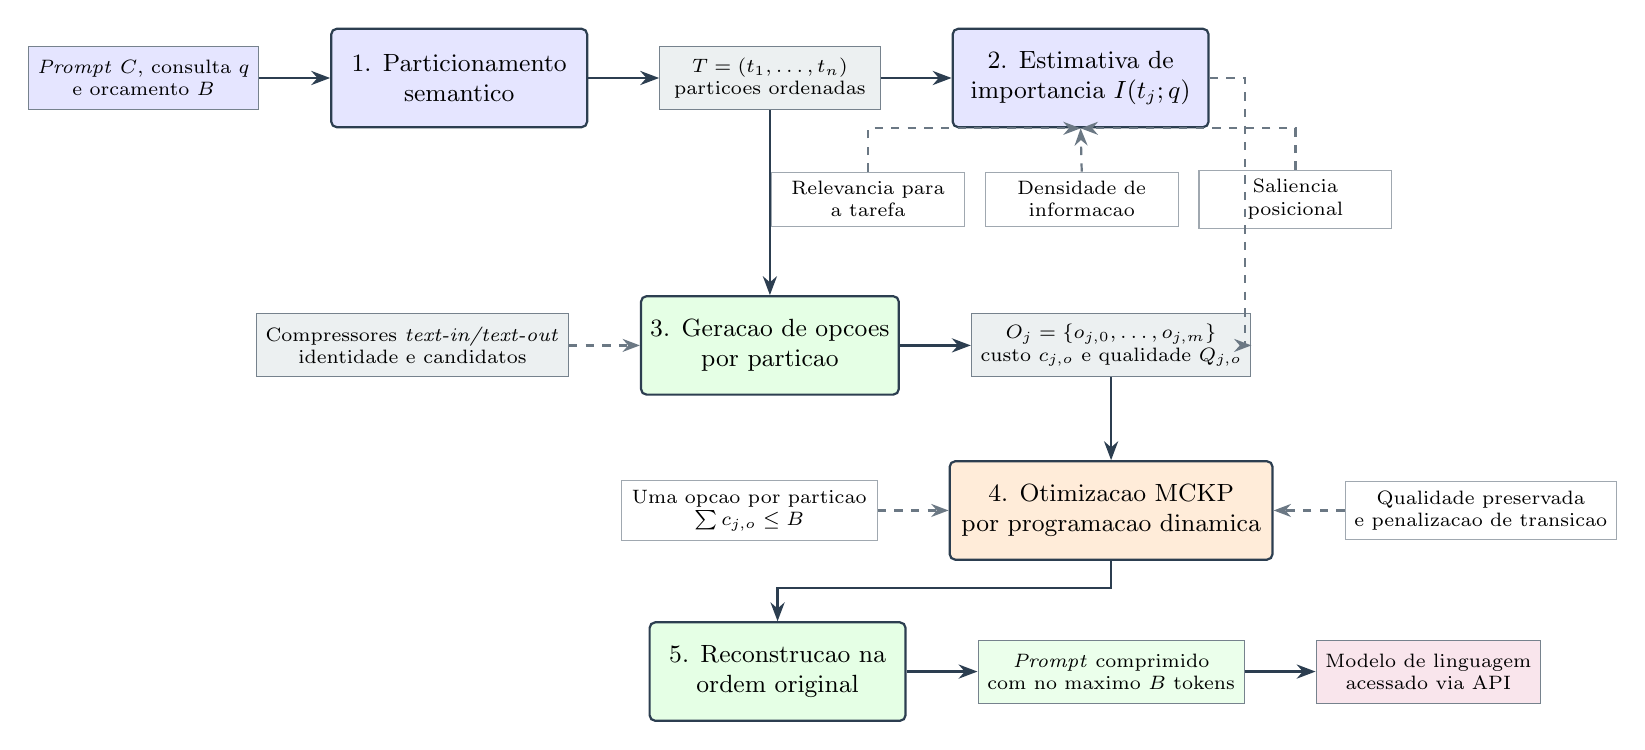
\begin{tikzpicture}[
    node distance=0.75cm and 0.9cm,
    stage/.style={rectangle, rounded corners=2pt, draw=dark, thick,
        minimum width=3.25cm, minimum height=1.25cm, align=center,
        font=\small, fill=white},
    artifact/.style={rectangle, draw=dark!65, minimum width=2.8cm,
        minimum height=0.8cm, align=center, font=\scriptsize, fill=light},
    detail/.style={rectangle, draw=dark!45, minimum width=2.45cm,
        minimum height=0.65cm, align=center, font=\scriptsize, fill=white},
    arrow/.style={-{Stealth[length=2.4mm]}, thick, draw=dark},
    dataarrow/.style={-{Stealth[length=2.2mm]}, thick, dashed, draw=dark!70}
]

% Entrada e analise do prompt
\node[artifact, fill=blue!10] (input) {\textit{Prompt} $C$, consulta $q$\\e orcamento $B$};
\node[stage, right=of input, fill=blue!10] (partition) {1. Particionamento\\semantico};
\node[artifact, right=of partition] (parts) {$T=(t_1,\ldots,t_n)$\\particoes ordenadas};
\node[stage, right=of parts, fill=blue!10] (importance) {2. Estimativa de\\importancia $I(t_j;q)$};

\draw[arrow] (input) -- (partition);
\draw[arrow] (partition) -- (parts);
\draw[arrow] (parts) -- (importance);

% Componentes da importancia
\node[detail, below=0.55cm of importance, xshift=-2.7cm] (relevance) {Relevancia para\\a tarefa};
\node[detail, right=0.25cm of relevance] (density) {Densidade de\\informacao};
\node[detail, right=0.25cm of density] (position) {Saliencia\\posicional};

\draw[dataarrow] (relevance.north) |- (importance.south);
\draw[dataarrow] (density.north) -- (importance.south);
\draw[dataarrow] (position.north) |- (importance.south);

% Geracao de opcoes
\node[stage, below=2.35cm of parts, fill=green!10] (options) {3. Geracao de opcoes\\por particao};
\node[artifact, left=of options, minimum width=3.25cm] (pool) {Compressores \textit{text-in/text-out}\\identidade e candidatos};
\node[artifact, right=of options, minimum width=3.25cm] (optiondata) {$O_j=\{o_{j,0},\ldots,o_{j,m}\}$\\custo $c_{j,o}$ e qualidade $Q_{j,o}$};

\draw[arrow] (parts.south) -- (options.north);
\draw[dataarrow] (importance.east) -- ++(0.45,0) |- (optiondata.east);
\draw[dataarrow] (pool) -- (options);
\draw[arrow] (options) -- (optiondata);

% Otimizacao e saida
\node[stage, below=1.05cm of optiondata, fill=orange!15, minimum width=4.1cm]
    (solver) {4. Otimizacao MCKP\\por programacao dinamica};
\node[detail, left=of solver, minimum width=3.25cm] (constraints)
    {Uma opcao por particao\\$\sum c_{j,o}\leq B$};
\node[detail, right=of solver, minimum width=3.25cm] (transition)
    {Qualidade preservada\\e penalizacao de transicao};

\draw[arrow] (optiondata) -- (solver);
\draw[dataarrow] (constraints) -- (solver);
\draw[dataarrow] (transition) -- (solver);

\node[artifact, below=1cm of solver, fill=green!8] (compressed)
    {\textit{Prompt} comprimido\\com no maximo $B$ tokens};
\node[stage, left=of compressed, fill=green!10] (rebuild)
    {5. Reconstrucao na\\ordem original};
\node[artifact, right=of compressed, fill=purple!10] (llm)
    {Modelo de linguagem\\acessado via API};

\draw[arrow] (solver.south) -- ++(0,-0.35) -| (rebuild.north);
\draw[arrow] (rebuild) -- (compressed);
\draw[arrow] (compressed) -- (llm);

\end{tikzpicture}%
}
\caption{Arquitetura conceitual do \textit{framework} proposto. O sistema transforma cada particao em alternativas com custo e qualidade, seleciona uma alternativa por particao sob o orcamento global e reconstrói o \textit{prompt} antes da chamada ao modelo.}
\label{fig:framework}
\end{figure}


\subsection{Particionamento e Orçamento}
\label{subsec:particionamento}

Seja $C$ o \textit{prompt} de entrada, com comprimento $|C|$ medido em \textit{tokens}. O \textit{framework} particiona $C$ em uma sequência de $n$ partições $T = (t_1, t_2, \ldots, t_n)$, de modo que cada partição corresponda a uma unidade semântica coerente, como uma instrução, uma pergunta, um documento recuperado ou um trecho de fundo. Define-se um orçamento efetivo de contexto $B \leq |C|$, que representa o número máximo de \textit{tokens} que o \textit{prompt} comprimido pode ocupar após a seleção das opções de compressão.

O particionador utilizado na execução principal é estrutural e produz unidades disjuntas, sem sobreposição entre trechos vizinhos. Parágrafos consecutivos são agrupados até o limite de 400 \textit{tokens}. Quando um parágrafo excede esse limite, ele é dividido por fronteiras de sentença; sentenças ainda maiores são separadas por palavras como último recurso. Esse procedimento preserva a cobertura do texto original e impede a duplicação de \textit{tokens}, condição necessária para que os custos das opções sejam aditivos. Uma variante de particionamento semântico permanece implementada, mas não integra a configuração principal. Para o controle uniforme, o contexto completo é representado como uma única partição.

\subsection{Função de Importância}
\label{subsec:importancia}

Para cada partição $t_j$, define-se uma função de importância $I(t_j; q)$ que quantifica a relevância da partição para a consulta $q$. A função combina múltiplos fatores por meio de uma soma ponderada, conforme a Equação~\ref{eq:importancia}.

\begin{equation}
\label{eq:importancia}
I(t_j; q) = \sum_{i} w_i \, \varphi_i(t_j, q),
\end{equation}

onde cada $\varphi_i(t_j, q)$ é um componente de relevância e $w_i$ é o peso associado. Os componentes considerados incluem a relevância da partição para a tarefa, a densidade de informação da partição e a saliência posicional, esta última motivada pelo viés \textit{lost in the middle} discutido na Seção~\ref{subsec:problema-critico}. A função de importância orienta a alocação de orçamento, atribuindo maior prioridade às partições cuja perda de conteúdo teria maior impacto sobre a resposta.

Na implementação atual, a relevância $R(t_j,q)$ combina similaridade semântica e sobreposição lexical. A similaridade semântica corresponde ao cosseno entre os \textit{embeddings} normalizados da partição e da consulta, produzidos pelo all-MiniLM-L6-v2. O componente lexical é calculado por TF-IDF. Os dois sinais são combinados segundo

\begin{equation}
\label{eq:relevancia-implementada}
R(t_j,q)=0.7\,R_{\mathrm{sem}}(t_j,q)+0.3\,R_{\mathrm{lex}}(t_j,q).
\end{equation}

A densidade factual $D(t_j)$ é aproximada pela proporção de ocorrências numéricas, datas e palavras iniciadas por letra maiúscula em relação ao número de palavras da partição. Esse componente constitui um indicador lexical de concentração factual, e não um reconhecedor de entidades. A saliência posicional $P(t_j)$ utiliza uma curva central, com valor maior para partições próximas ao centro da sequência:

\begin{equation}
\label{eq:saliencia-central}
P(t_j)=1-\left|2\frac{j-1}{n-1}-1\right|,
\end{equation}

para $n>1$. Antes da combinação, $R$, $D$ e $P$ são normalizados por \textit{min--max} entre as partições da mesma entrada. Quando todos os valores de um componente são iguais, o componente normalizado recebe valor 1 em todas as partições. Com os pesos da configuração experimental, a função efetivamente utilizada é

\begin{equation}
\label{eq:importancia-implementada}
I(t_j;q)=0.6\,\widehat{R}(t_j,q)
        +0.2\,\widehat{D}(t_j)
        +0.2\,\widehat{P}(t_j),
\end{equation}

onde o acento circunflexo indica o valor normalizado. Os pesos são mantidos fixos na execução principal e tratados como componentes sujeitos a ablação, uma vez que sua combinação representa uma hipótese operacional sobre relevância, densidade e posição.

\subsection{Opções de Compressão e Modelo de Qualidade}
\label{subsec:opcoes}

Para cada partição $t_j$, o \textit{framework} considera um conjunto de opções de compressão $O_j = \{o_{j,0}, o_{j,1}, \ldots, o_{j,m}\}$. Cada opção $o = (A_k, p)$ corresponde à aplicação de um compressor $A_k$ com um parâmetro de operação $p$, como uma taxa de compressão alvo. A opção $o_{j,0}$ corresponde ao compressor identidade $A_0$, que preserva a partição integralmente e serve de referência para o custo e a qualidade máximos daquela partição.

Cada opção possui um custo $c_{j,o}$, medido pelo número de \textit{tokens} da partição após a compressão, e uma qualidade $Q_{j,o}$, que estima a informação preservada pela opção. A qualidade combina a importância da partição com a fidelidade da opção de compressão, conforme a Equação~\ref{eq:qualidade}.

\begin{equation}
\label{eq:qualidade}
Q_{j,o} = I(t_j; q) \cdot f_{j,o},
\end{equation}

onde $f_{j,o} \in [0,1]$ representa a fração de informação da partição preservada pela opção $o$. O compressor identidade satisfaz $f_{j,0} = 1$, e opções mais agressivas apresentam valores menores de $f_{j,o}$, capturando o compromisso entre redução de \textit{tokens} e perda de conteúdo.

Na implementação atual, a fidelidade semântica é calculada por cobertura entre \textit{embeddings}. A partição original e sua representação comprimida são divididas em trechos de 600 caracteres. Para limitar o custo, no máximo 48 trechos de cada texto são mantidos por amostragem uniforme. Seja $S_j$ o conjunto de trechos da partição original e $S'_{j,o}$ o conjunto correspondente à opção comprimida. A fidelidade semântica é

\begin{equation}
\label{eq:fidelidade-semantica-implementada}
f^{\mathrm{sem}}_{j,o}
=
\frac{1}{|S_j|}
\sum_{s\in S_j}
\max_{u\in S'_{j,o}}
\cos\bigl(E(s),E(u)\bigr),
\end{equation}

onde $E(\cdot)$ é o codificador all-MiniLM-L6-v2. A medida estima quanto do conteúdo semântico de cada trecho original encontra uma representação próxima no texto comprimido. Ela não utiliza a resposta esperada do \textit{benchmark}, evitando que informação do conjunto de avaliação seja incorporada à decisão do MCKP.

Como proteção factual adicional, calcula-se a retenção numérica $r^{\mathrm{num}}_{j,o}$, definida como a fração de números, datas, percentuais, valores e horários da partição original que permanecem na opção comprimida. Quando essa retenção é aplicável e fica abaixo do limiar de 0.9, a fidelidade da opção é ajustada por

\begin{equation}
\label{eq:fidelidade-ajustada}
f_{j,o}
=
\min\left(f^{\mathrm{sem}}_{j,o},r^{\mathrm{num}}_{j,o}\right).
\end{equation}

Nos demais casos, $f_{j,o}=f^{\mathrm{sem}}_{j,o}$. A identidade recebe fidelidade 1 e a omissão recebe fidelidade 0. O conjunto principal de opções contém identidade, omissão, CPC-MiniLM, LLMLingua-2 e Selective Context. Os três compressores são materializados com taxas nominais de retenção de 0.5 e 0.3. Se o custo serializado das identidades exceder o orçamento, acrescenta-se a cada compressor uma taxa adaptativa

\begin{equation}
\label{eq:taxa-adaptativa}
\rho_{\mathrm{adapt}}
=
\max\left(0.05,
\min\left(1,\;0.9\frac{B}{C_{\mathrm{id}}}\right)\right),
\end{equation}

onde $C_{\mathrm{id}}$ é o custo total das partições sem compressão. A taxa mínima de 0.05 também é avaliada quando difere da taxa adaptativa. O custo $c_{j,o}$ é medido após a materialização da opção e inclui, de forma conservadora, o separador empregado na reconstrução. Assim, a taxa solicitada ao compressor não substitui a medição do custo efetivamente produzido.

\subsection{Restrições de Compatibilidade}
\label{subsec:compatibilidade}

Nem toda combinação de opções entre partições adjacentes é adequada, pois transições abruptas de estilo ou de nível de compressão entre trechos vizinhos podem prejudicar a coerência do \textit{prompt} reconstruído. Define-se uma função de compatibilidade $M(o, o')$ entre opções de partições adjacentes, que penaliza combinações incompatíveis. A compatibilidade é incorporada como uma penalização de transição na função objetivo, por meio de um termo $\mu \sum_{j} d(o_j, o_{j+1})$, onde $d(\cdot, \cdot)$ mede a distância entre opções adjacentes e $\mu$ controla a intensidade da penalização.

Na configuração principal, a distância depende da família do compressor:

\begin{equation}
\label{eq:distancia-familia}
d(o,o')=
\begin{cases}
0, & \text{se } A(o)=A(o'),\\
1, & \text{caso contrário},
\end{cases}
\end{equation}

onde $A(o)$ identifica o compressor associado à opção. O valor principal é $\mu=0.1$, interpretado como uma regularização equivalente a 10\% da escala unitária de valor para cada troca de família entre partições adjacentes. Esse valor constitui uma escolha inicial do protocolo, e não um parâmetro derivado da formulação. As execuções com $\mu=0$ e $\mu=0.5$ são mantidas como ablações para distinguir o MCKP clássico de uma penalização mais intensa.

\subsection{Formulação como Extensão do Problema da Mochila de Múltipla Escolha}
\label{subsec:mckp}

A seleção das opções de compressão é formulada como uma extensão do MCKP com penalização entre escolhas adjacentes. Para cada partição $t_j$ e cada opção $o \in O_j$, define-se uma variável binária $x_{j,o} \in \{0,1\}$, que assume o valor 1 quando a opção $o$ é escolhida para a partição $t_j$. Denota-se por $o_j$ a única opção cuja variável assume valor 1 na partição $j$. O problema consiste em maximizar a qualidade total preservada sujeita ao orçamento e à escolha de exatamente uma opção por partição, conforme as Equações~\ref{eq:mckp-obj} a \ref{eq:mckp-bin}. Quando $\mu=0$, a formulação se reduz ao MCKP clássico; quando $\mu>0$, o termo de transição incorpora a coerência entre partições vizinhas.

\begin{align}
\max_{x} \quad & \sum_{j=1}^{n} \sum_{o \in O_j} x_{j,o} \, Q_{j,o}
    - \mu \sum_{j=1}^{n-1} d(o_j, o_{j+1}) \label{eq:mckp-obj} \\
\text{s.a.} \quad & \sum_{j=1}^{n} \sum_{o \in O_j} x_{j,o} \, c_{j,o} \leq B \label{eq:mckp-orc} \\
& \sum_{o \in O_j} x_{j,o} = 1, \quad j = 1, \ldots, n \label{eq:mckp-um} \\
& x_{j,o} \in \{0,1\}. \label{eq:mckp-bin}
\end{align}

A Equação~\ref{eq:mckp-obj} maximiza a qualidade total preservada, descontada da penalização de transição entre partições adjacentes. A Equação~\ref{eq:mckp-orc} impõe o orçamento efetivo de contexto. A Equação~\ref{eq:mckp-um} garante que exatamente uma opção seja escolhida por partição, característica que distingue o núcleo MCKP do problema da mochila clássico.

\subsection{Solução por Programação Dinâmica}
\label{subsec:dp}

O MCKP com orçamento inteiro admite solução por programação dinâmica. Como a função objetivo inclui uma penalização entre opções adjacentes, o estado também deve registrar a opção escolhida para a última partição. Define-se $D[j,b,o]$ como a qualidade máxima preservada considerando as $j$ primeiras partições sob um orçamento parcial $b$, quando a opção $o\in O_j$ é escolhida para a partição $t_j$. A recorrência é apresentada na Equação~\ref{eq:dp}.

\begin{equation}
\label{eq:dp}
D[j,b,o] = Q_{j,o} + \max_{o' \in O_{j-1}}
\Big\{D[j-1,b-c_{j,o},o'] - \mu\,d(o',o)\Big\},
\end{equation}

Para a primeira partição, define-se $D[1,b,o]=Q_{1,o}$ quando $c_{1,o}\leq b$, e $D[1,b,o]=-\infty$ caso contrário. A solução ótima corresponde a $\max_{o\in O_n}D[n,B,o]$, e as opções escolhidas são recuperadas por retrocesso (\textit{backtracking}) sobre a tabela de decisão. Para no máximo $m$ opções por partição, a complexidade temporal é $O(nBm^2)$ e a tabela completa ocupa $O(nBm)$ posições; a memória pode ser reduzida quando apenas o valor ótimo, sem o retrocesso, é necessário.

Na implementação de referência, o eixo de orçamento utiliza unidades inteiras de \textit{tokens} (\texttt{budget\_bucket=1}), preservando a solução exata para o modelo de custos declarado. Uma quantização opcional por blocos permanece disponível como aproximação conservadora para instâncias maiores, mas não é utilizada nos experimentos principais. Os custos das opções incluem a serialização necessária à reconstrução, e o contexto final é recontado antes da chamada ao modelo para verificar a restrição de orçamento.

A Figura~\ref{fig:mckp-dp-flow} detalha o fluxo proposto para o preenchimento da tabela de programação dinâmica e para a recuperação das opções selecionadas.

% Fluxo conceitual da solucao do MCKP por programacao dinamica.

\begin{figure}[htbp]
\centering
\resizebox{!}{0.70\textheight}{%
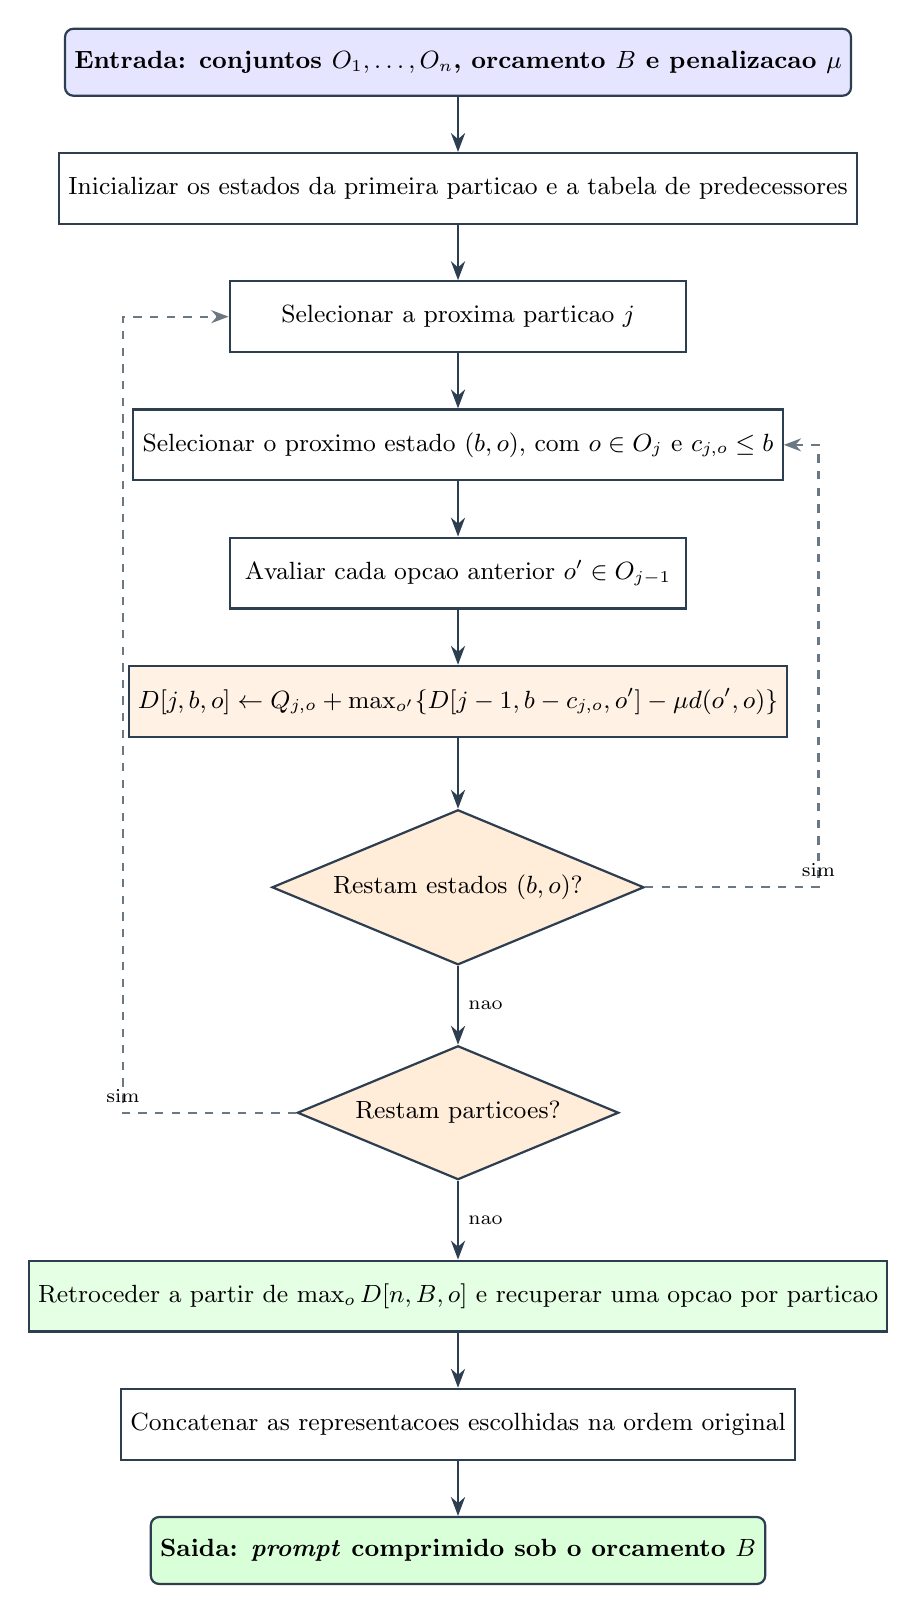
\begin{tikzpicture}[
    node distance=0.7cm,
    startstop/.style={rectangle, rounded corners=3pt, draw=dark, thick,
        minimum width=4.8cm, minimum height=0.85cm, align=center,
        font=\small\bfseries, fill=blue!10},
    process/.style={rectangle, draw=dark, thick, minimum width=5.8cm,
        minimum height=0.9cm, align=center, font=\small, fill=white},
    decision/.style={diamond, aspect=2.4, draw=dark, thick,
        minimum width=3.4cm, minimum height=0.85cm, align=center,
        font=\small, fill=orange!15},
    arrow/.style={-{Stealth[length=2.4mm]}, thick, draw=dark},
    loop/.style={-{Stealth[length=2.2mm]}, thick, dashed, draw=dark!70}
]

\node[startstop] (start) {Entrada: conjuntos $O_1,\ldots,O_n$, orcamento $B$ e penalizacao $\mu$};
\node[process, below=of start] (init) {Inicializar os estados da primeira particao e a tabela de predecessores};
\node[process, below=of init] (part) {Selecionar a proxima particao $j$};
\node[process, below=of part] (budget) {Selecionar o proximo estado $(b,o)$, com $o\in O_j$ e $c_{j,o}\leq b$};
\node[process, below=of budget] (evaluate) {Avaliar cada opcao anterior $o'\in O_{j-1}$};
\node[process, below=of evaluate, fill=orange!10] (update)
    {$D[j,b,o]\leftarrow Q_{j,o}+\max_{o'}\{D[j-1,b-c_{j,o},o']-\mu d(o',o)\}$};
\node[decision, below=0.9cm of update] (moreb) {Restam estados $(b,o)$?};
\node[decision, below=1cm of moreb] (morej) {Restam particoes?};
\node[process, below=1cm of morej, fill=green!10] (backtrack)
    {Retroceder a partir de $\max_o D[n,B,o]$ e recuperar uma opcao por particao};
\node[process, below=of backtrack] (rebuild)
    {Concatenar as representacoes escolhidas na ordem original};
\node[startstop, below=of rebuild, fill=green!15] (end)
    {Saida: \textit{prompt} comprimido sob o orcamento $B$};

\draw[arrow] (start) -- (init);
\draw[arrow] (init) -- (part);
\draw[arrow] (part) -- (budget);
\draw[arrow] (budget) -- (evaluate);
\draw[arrow] (evaluate) -- (update);
\draw[arrow] (update) -- (moreb);
\draw[loop] (moreb.east) -- ++(2.2,0) node[above, font=\scriptsize] {sim} |- (budget.east);
\draw[arrow] (moreb) -- node[right, font=\scriptsize] {nao} (morej);
\draw[loop] (morej.west) -- ++(-2.2,0) node[above, font=\scriptsize] {sim} |- (part.west);
\draw[arrow] (morej) -- node[right, font=\scriptsize] {nao} (backtrack);
\draw[arrow] (backtrack) -- (rebuild);
\draw[arrow] (rebuild) -- (end);

\end{tikzpicture}%
}
\caption{Fluxo proposto para resolver a selecao de compressores por programacao dinamica. A tabela registra a melhor qualidade acumulada para cada particao, orcamento parcial e ultima opcao; o retrocesso recupera as opcoes usadas na reconstrucao.}
\label{fig:mckp-dp-flow}
\end{figure}


\subsection{Algoritmo do \textit{Framework}}
\label{subsec:algoritmo}

O funcionamento do \textit{framework} pode ser resumido em cinco etapas encadeadas.

\begin{enumerate}[leftmargin=1.8em]
\item \textbf{Particionamento}. O \textit{prompt} $C$ é dividido em partições $T = (t_1, \ldots, t_n)$ segundo unidades semânticas coerentes.

\item \textbf{Estimativa de importância}. Para cada partição, calcula-se a importância $I(t_j; q)$ segundo a Equação~\ref{eq:importancia}.

\item \textbf{Geração de opções}. Para cada partição, aplica-se o conjunto de compressores candidatos, produzindo opções com seus custos $c_{j,o}$ e qualidades $Q_{j,o}$.

\item \textbf{Otimização}. Resolve-se a extensão do MCKP das Equações~\ref{eq:mckp-obj} a \ref{eq:mckp-bin} por programação dinâmica, respeitando o orçamento $B$ e as restrições de compatibilidade.

\item \textbf{Reconstrução}. As opções escolhidas são concatenadas na ordem original das partições, produzindo o \textit{prompt} comprimido enviado ao modelo.
\end{enumerate}

A Figura~\ref{fig:sequence-diagram} apresenta a sequência de interação implementada entre os componentes necessários para executar essas etapas.

% Sequencia conceitual entre os componentes do framework proposto.

\begin{figure}[htbp]
\centering
\resizebox{0.98\textwidth}{!}{%
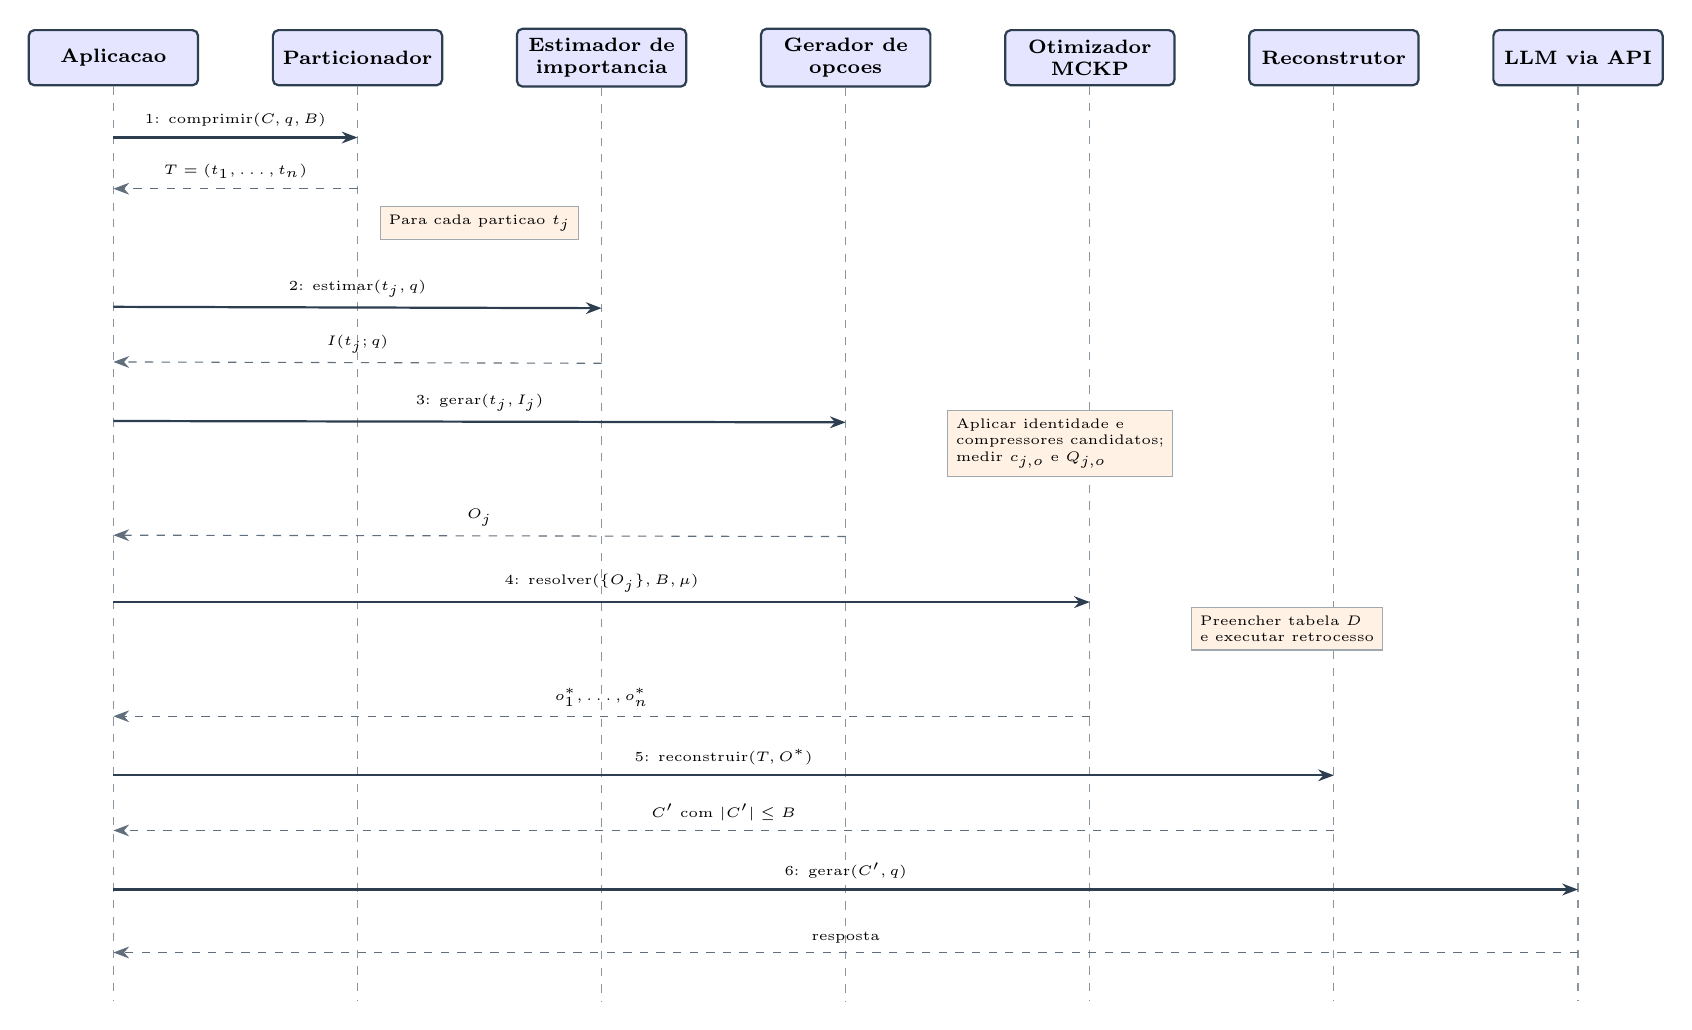
\begin{tikzpicture}[
    actor/.style={rectangle, rounded corners=2pt, minimum width=2.15cm,
        minimum height=0.7cm, draw=dark, thick, fill=blue!10,
        font=\scriptsize\bfseries, align=center},
    lifeline/.style={dashed, draw=dark!55},
    message/.style={-{Stealth[length=2mm]}, thick, draw=dark},
    return/.style={-{Stealth[length=2mm]}, dashed, draw=dark!75},
    note/.style={rectangle, draw=dark!45, fill=orange!10,
        font=\tiny, align=left, inner sep=3pt}
]

\node[actor] (app) at (0,0) {Aplicacao};
\node[actor] (partitioner) at (3.1,0) {Particionador};
\node[actor] (estimator) at (6.2,0) {Estimador de\\importancia};
\node[actor] (pool) at (9.3,0) {Gerador de\\opcoes};
\node[actor] (solver) at (12.4,0) {Otimizador\\MCKP};
\node[actor] (assembler) at (15.5,0) {Reconstrutor};
\node[actor] (llm) at (18.6,0) {LLM via API};

\foreach \x in {app,partitioner,estimator,pool,solver,assembler,llm} {
    \draw[lifeline] (\x.south) -- ++(0,-11.6);
}

\draw[message] ([yshift=-0.65cm]app.south) -- node[above, font=\tiny] {1: comprimir$(C,q,B)$} ([yshift=-0.65cm]partitioner.south);
\draw[return] ([yshift=-1.3cm]partitioner.south) -- node[above, font=\tiny] {$T=(t_1,\ldots,t_n)$} ([yshift=-1.3cm]app.south);

\node[note] at (4.65,-2.1) {Para cada particao $t_j$};
\draw[message] ([yshift=-2.8cm]app.south) -- node[above, font=\tiny] {2: estimar$(t_j,q)$} ([yshift=-2.8cm]estimator.south);
\draw[return] ([yshift=-3.5cm]estimator.south) -- node[above, font=\tiny] {$I(t_j;q)$} ([yshift=-3.5cm]app.south);

\draw[message] ([yshift=-4.25cm]app.south) -- node[above, font=\tiny] {3: gerar$(t_j,I_j)$} ([yshift=-4.25cm]pool.south);
\node[note, right=0.2cm of pool, yshift=-4.9cm] {Aplicar identidade e\\compressores candidatos;\\medir $c_{j,o}$ e $Q_{j,o}$};
\draw[return] ([yshift=-5.7cm]pool.south) -- node[above, font=\tiny] {$O_j$} ([yshift=-5.7cm]app.south);

\draw[message] ([yshift=-6.55cm]app.south) -- node[above, font=\tiny] {4: resolver$(\{O_j\},B,\mu)$} ([yshift=-6.55cm]solver.south);
\node[note, right=0.2cm of solver, yshift=-7.25cm] {Preencher tabela $D$\\e executar retrocesso};
\draw[return] ([yshift=-8cm]solver.south) -- node[above, font=\tiny] {$o_1^*,\ldots,o_n^*$} ([yshift=-8cm]app.south);

\draw[message] ([yshift=-8.75cm]app.south) -- node[above, font=\tiny] {5: reconstruir$(T,O^*)$} ([yshift=-8.75cm]assembler.south);
\draw[return] ([yshift=-9.45cm]assembler.south) -- node[above, font=\tiny] {$C'$ com $|C'|\leq B$} ([yshift=-9.45cm]app.south);

\draw[message] ([yshift=-10.2cm]app.south) -- node[above, font=\tiny] {6: gerar$(C',q)$} ([yshift=-10.2cm]llm.south);
\draw[return] ([yshift=-11cm]llm.south) -- node[above, font=\tiny] {resposta} ([yshift=-11cm]app.south);

\end{tikzpicture}%
}
\caption{Sequencia conceitual da aplicacao do \textit{framework}. Para cada particao, sao calculadas a importancia e as alternativas de compressao; o otimizador seleciona as alternativas globalmente antes da reconstrucao e da chamada ao modelo.}
\label{fig:framework-sequence}
\end{figure}


\subsection{Conjunto de Compressores Compatíveis}
\label{subsec:pool}

O \textit{framework} atua como uma camada de decisão acima de compressores existentes, e não como um novo compressor. Por essa razão, o conjunto de opções por partição é composto por compressores do tipo \textit{text-in}/\textit{text-out}, isto é, que recebem texto e produzem texto comprimido, o que garante compatibilidade com modelos acessados via API. LLMLingua é empregado como baseline externo, pois constitui o ponto de comparação comum aos três trabalhos posteriores revisados na Seção~\ref{subsec:compressao-prompt}. LLMLingua-2, Selective Context e CPC são avaliados como candidatos às opções do MCKP. A Tabela~\ref{tab:compressores} resume os respectivos papéis experimentais.

\begin{table}[htbp]
\centering
\caption{Baseline e compressores candidatos considerados para o MCKP}
\label{tab:compressores}
\begin{tabular}{>{\raggedright\arraybackslash}p{3.2cm}>{\raggedright\arraybackslash}p{2.5cm}>{\raggedright\arraybackslash}p{6.0cm}}
\toprule
\textbf{Compressor} & \textbf{Papel} & \textbf{Característica relevante} \\
\midrule
Identidade ($A_0$) & Referência interna & Preserva a partição integralmente, com fidelidade máxima. \\
\addlinespace
LLMLingua-GPT2 \cite{jiang2023llmlingua} & Baseline com \textit{scorer} adaptado & Implementação do pacote \texttt{llmlingua}, com GPT-2 em CPU para reduzir o custo local. \\
\addlinespace
LLMLingua-2 \cite{pan2024llmlingua2} & Candidato MCKP & Classificação de palavras treinada por destilação, agnóstica à pergunta e com baixa latência. \\
\addlinespace
Selective Context \cite{li2023selective} & Candidato MCKP & Remoção de unidades lexicais por auto-informação, sem treinamento específico. \\
\addlinespace
CPC-MiniLM \cite{li2024cpc} & Aproximação candidata & Seleção de sentenças condicionada à pergunta com \textit{embeddings} do all-MiniLM-L6-v2. \\
\bottomrule
\end{tabular}
\end{table}

A recomendação dos três candidatos se baseia em sua complementaridade. LLMLingua-2 opera em nível de palavra e amortiza o custo de compressão entre consultas, Selective Context introduz uma alternativa sem treinamento específico e CPC-MiniLM preserva sentenças completas com seleção condicionada à pergunta. A escolha por compressores \textit{text-in}/\textit{text-out} mantém a propriedade não invasiva do \textit{framework}, pois nenhuma etapa exige acesso aos parâmetros internos, retreinamento ou modificação arquitetural do modelo base. O conjunto candidato pode ser estendido com outros compressores compatíveis sem alteração da formulação, uma vez que cada compressor é incorporado apenas como uma nova opção por partição. Nas dez combinações de modelo e orçamento, CPC-MiniLM apresenta a maior média entre os quatro compressores em oito, enquanto LLMLingua-2 lidera nas duas combinações do Qwen 3 30B-A3B. Selective Context preserva a maior fidelidade semântica segundo a métrica adotada. Esses resultados sustentam LLMLingua-2, Selective Context e CPC-MiniLM como conjunto inicial de opções do MCKP; LLMLingua-GPT2 permanece como baseline externo. Os resultados são apresentados na Seção~\ref{subsec:resultados-triagem-compressores}.

Na configuração primária definida na Seção~\ref{subsec:selecao-modelo-mckp}, com Llama~3.1 8B e janela de 8.192 tokens, CPC-MiniLM também foi o compressor individual com melhor resultado downstream. Nos 22 casos da matriz exploratória, obteve médias macro e micro de 0,531 e 0,538, respectivamente, com latência média de 6,74~s e retenção de 0,517. LLMLingua-2 atingiu média macro de 0,492 e a menor retenção (0,457), enquanto Selective Context alcançou média macro de 0,480 e a maior fidelidade semântica (0,733). LLMLingua-GPT2 obteve média macro de 0,379. Portanto, CPC-MiniLM é adotado como referência primária quando se exige um único compressor, sem excluir os demais do espaço de decisão do MCKP, pois suas características complementares podem ser úteis para segmentos específicos. Esses valores são tratados como evidência exploratória, uma vez que a matriz contém uma execução por caso e utiliza instâncias sintéticas nos conjuntos derivados do LongBench.

\subsection{Implementação de Referência}
\label{subsec:implementacao}

O repositório contém uma implementação integrada no subdiretório \texttt{mckp}. O módulo \path{partitioner.py} produz partições disjuntas; \path{importance.py} calcula $I(t_j;q)$; \path{options.py} materializa e avalia as opções; \path{solver.py} executa a programação dinâmica e o retrocesso; e \path{reconstructor.py} preserva a ordem das opções selecionadas sem introduzir marcadores não contabilizados. A classe \texttt{MCKPStrategy}, em \path{strategy.py}, coordena essas etapas e expõe a estratégia ao executor de \textit{benchmarks}.

\paragraph{Separação em relação à etapa inicial da matriz local.}
A estratégia denominada \textit{Semantic Compression} na etapa inicial da matriz local não implementava LLMLingua. Em vez disso, ela solicitava que a própria LLM reescrevesse o contexto por meio de uma instrução de compressão, conforme a abordagem de Gilbert et al. \cite{gilbert2023semanticcompression}. O repositório também continha um \texttt{PerplexityCompressor} experimental, que selecionava \textit{tokens} pela perda calculada com GPT-2 e podia ser descrito apenas como inspirado no critério do LLMLingua. Esse protótipo não estava registrado entre as estratégias avaliadas. Para a ampliação da matriz foram criadas entradas explícitas e independentes para LLMLingua, LLMLingua-2, Selective Context e CPC-MiniLM. Assim, resultados da \textit{Semantic Compression} ou do protótipo de perplexidade não são apresentados como resultados de LLMLingua.

\paragraph{Adaptações para execução local.}
Os experimentos utilizam uma LLM alvo executada localmente pelo servidor Ollama 0.32.3, de modo que o compressor e o modelo gerador compartilham os recursos computacionais da mesma máquina. Cada chamada informa explicitamente \texttt{num\_ctx}, reserva até 500 \textit{tokens} para a saída, utiliza temperatura 0 e fixa a semente em 42. O orçamento do MCKP desconta da janela o \textit{template} completo sem contexto, a consulta, a reserva de saída e uma margem de segurança de 256 \textit{tokens}. O contexto reconstruído e o \textit{prompt} final são recontados antes da chamada, enquanto a contagem real reportada pelo Ollama é registrada para avaliar a diferença entre o contador da otimização e o tokenizador do modelo alvo.

O baseline invoca a classe \texttt{PromptCompressor} do pacote \texttt{llmlingua} 0.2.2, com \texttt{use\_llmlingua2=False}, taxa de retenção de 0,5 e execução em CPU. Para reduzir a concorrência de memória com os modelos servidos pelo Ollama, o modelo causal auxiliar é o \texttt{gpt2} \cite{radford2019gpt2}, que já se encontrava no \textit{cache} local e é substancialmente menor que um auxiliar de 7 bilhões de parâmetros. A escolha é compatível com a arquitetura do LLMLingua e com a análise de diferentes modelos auxiliares apresentada por Jiang et al. \cite{jiang2023llmlingua}; entretanto, difere das configurações alinhadas, Alpaca-7B e GPT2-Alpaca, avaliadas no artigo. Por isso, a configuração é reportada como \textbf{LLMLingua-GPT2}, uma vez que o algoritmo provém da implementação do LLMLingua, enquanto o \textit{scorer} não ajustado e o dispositivo são escolhas locais que devem acompanhar a interpretação dos resultados.

LLMLingua-2 também é executado pelo pacote \texttt{llmlingua} 0.2.2, com o \textit{checkpoint} \path{microsoft/llmlingua-2-xlm-roberta-large-meetingbank} e \texttt{device\_map=cpu}. A fixação explícita do dispositivo foi necessária porque a inicialização padrão do pacote pressupunha CUDA, indisponível nessa configuração. A biblioteca Transformers foi fixada na versão 4.46.3, pois o LLMLingua 0.2.2 manipula o formato legado do \textit{cache} de chaves e valores; a versão 5.12.1 instalada inicialmente passou a retornar \texttt{DynamicCache} e provocava falhas durante a compressão iterativa. Selective Context é executado pelo pacote \texttt{selective-context} 0.1.4 com GPT-2, idioma inglês e \texttt{reduce\_ratio=1-rate}, pois sua API recebe a fração removida, ao passo que o executor comum recebe a fração retida. Essa integração utiliza spaCy 3.8.14 e o modelo \texttt{en\_core\_web\_sm} 3.8.0 para o processamento linguístico.

Uma adaptação análoga foi necessária para o CPC. O trabalho original ajusta um Mistral-7B-Instruct com o conjunto CQR para produzir representações de sentenças condicionadas ao contexto \cite{li2024cpc}. O repositório oficial disponibiliza o código, o conjunto CQR e compressores pré-treinados baseados em Mistral-7B e Llama-1B \cite{workday2025cpc}; ainda assim, acrescentar outro modelo desse porte à mesma máquina ampliaria a disputa de memória com as LLMs locais avaliadas. Na triagem experimental, o codificador é, portanto, substituído pelo all-MiniLM-L6-v2, da coleção Sentence Transformers no Hugging Face \cite{huggingface2022allminilm}. O compressor divide a partição em sentenças, calcula separadamente os \textit{embeddings} das sentenças e da pergunta, ordena as sentenças pela similaridade de cosseno e preserva as mais relevantes dentro da taxa de retenção, mantendo a ordem textual original. Essa variante é denominada CPC-MiniLM. Ela preserva a seleção extrativa em nível de sentença e o condicionamento à pergunta, mas não incorpora o treinamento contrastivo nem a representação contextual do CPC original. Consequentemente, trata-se de uma aproximação operacional, e diferenças de qualidade e latência entre CPC-MiniLM e os demais compressores não devem ser atribuídas diretamente ao método publicado por Liskavets et al. \cite{li2024cpc}.

\paragraph{Rastreabilidade da triagem.}
As quatro estratégias adicionadas são executadas somente quando nomeadas explicitamente e não foram incluídas no grupo \texttt{all}; essa decisão preserva a reprodutibilidade da etapa inicial da matriz local. A triagem usa o ambiente \texttt{.venv}, que contém as dependências dos quatro compressores, e grava seus artefatos em \path{tests/ollama-local/benchmark_matrix_compressores}, separado de \path{benchmark_matrix_artigo}. O protocolo completo prevê os cinco modelos, os orçamentos de 8192 e 32768 \textit{tokens}, os sete \textit{benchmarks} e a taxa de retenção de 0,5. O modo \texttt{quick} materializa três casos de resposta a perguntas e um caso de sumarização no LongBench, enquanto cada um dos outros seis arquivos locais contém três exemplos, totalizando 22 casos por estratégia e 88 resultados por combinação de modelo e orçamento.

Os artefatos consolidados reúnem as dez combinações de modelo e orçamento, correspondentes aos cinco modelos avaliados com 8192 e 32768 \textit{tokens}. Cada combinação registra 88 execuções, resultantes da aplicação dos quatro compressores aos mesmos 22 casos, totalizando 880 observações. Uma geração de resposta do CPC-MiniLM com o DeepSeek-R1 32B em 8192 \textit{tokens}, no caso \texttt{meeting\_summarization\_0}, terminou por \textit{timeout}. A saída de erro não foi tratada como resposta e foi excluída das médias de pontuação e latência, de modo que essas duas métricas reúnem 879 respostas válidas; a taxa retida e a fidelidade dessa execução permanecem válidas, pois a compressão foi concluída antes da chamada ao modelo alvo. A execução utiliza um processo por combinação de modelo e orçamento, no qual as quatro estratégias são registradas conjuntamente; assim, os auxiliares GPT-2 (LLMLingua-GPT2), XLM-RoBERTa (LLMLingua-2), GPT-2 (Selective Context) e MiniLM (CPC-MiniLM) podem coexistir durante a rodada. O processo é encerrado antes da combinação seguinte, liberando o modelo alvo e os auxiliares. Essa organização preserva a comparabilidade de qualidade dentro de cada combinação, mas as latências devem ser interpretadas como custo descritivo de ponta a ponta no ambiente local, e não como medição isolada do custo de cada compressor.

O orçamento é derivado independentemente para as janelas de 8192 e 32768 \textit{tokens}. Em cada rodada são descontados o \textit{template} completo, a pergunta, a reserva de saída e uma margem de segurança para diferenças entre o contador \textit{tiktoken} usado nas métricas e o tokenizador do modelo alvo. A implementação registra o custo previsto pelo resolvedor, o custo recontado do contexto final, o orçamento não utilizado e eventuais compressores indisponíveis, permitindo auditar cada execução.

\subsection{Aplicação da Solução de Ponta a Ponta}
\label{subsec:aplicacao}

Esta subseção rastreia um caso concreto por todos os estágios do \textit{framework}, de modo a tornar explícito o funcionamento descrito nas subseções anteriores. O caso provém do HotpotQA e foi processado sob a configuração principal, com o Llama 3.1 8B e orçamento de 8192 \textit{tokens}. A pergunta é ``Are the Laleli Mosque and Esma Sultan Mansion located in the same neighborhood?'', e o contexto reúne passagens sobre entidades otomanas, das quais apenas uma contém a informação necessária para a resposta.

O particionamento estrutural produz três partições disjuntas do tipo \textit{paragraph\_group}. A função de importância pontua cada partição pela combinação de relevância à pergunta, densidade de informação e saliência posicional, com os pesos 0,6, 0,2 e 0,2 definidos na Seção~\ref{subsec:importancia}. A Tabela~\ref{tab:exemplo-particoes} apresenta a decomposição da importância. A partição 2 reúne os verbetes da Laleli Mosque e da Esma Sultan Mansion e recebe relevância e densidade máximas, o que a torna a partição de maior importância. A partição 1 obtém saliência posicional máxima por ocupar a região central da entrada, enquanto a partição 0 apresenta relevância intermediária.

\begin{table}[htbp]
\centering
\caption{Particionamento e decomposição da importância no caso analisado}
\label{tab:exemplo-particoes}
\begin{tabular}{cccccc}
\toprule
\textbf{Partição} & \textbf{Caracteres} & \textbf{Relevância} & \textbf{Densidade} & \textbf{Saliência} & \textbf{Importância} \\
\midrule
0 & 1201 & 0,384 & 0,000 & 0,000 & 0,231 \\
1 & 1394 & 0,000 & 0,313 & 1,000 & 0,263 \\
2 & 1013 & 1,000 & 1,000 & 0,000 & \textbf{0,800} \\
\bottomrule
\end{tabular}
\end{table}

Para cada partição, o gerador materializa as opções de compressão e calcula, por opção, o custo em \textit{tokens}, a fidelidade e o valor $Q = I(t_j;q)\,f_{j,o}$. O conjunto reúne a cópia integral, a omissão e os compressores CPC-MiniLM e LLMLingua-2 nas taxas de 0,7, 0,5 e 0,3. A Tabela~\ref{tab:exemplo-opcoes} lista essas opções e destaca a escolhida pelo resolvedor em cada partição. Como a fidelidade multiplica a importância, a cópia integral concentra o maior valor nas três partições. As opções comprimidas ilustram, contudo, a heterogeneidade dos compressores descrita na Seção~\ref{subsec:pool}. Na partição 2, o LLMLingua-2 com taxa 0,7 alcança fidelidade de 0,843 e valor de 0,674, enquanto o CPC-MiniLM na mesma taxa obtém fidelidade de 0,500 e valor de 0,400. Sob pressão de orçamento, essa diferença de valor por \textit{token} leva o resolvedor a preferir o LLMLingua-2 nessa partição.

{
\footnotesize
\setlength{\tabcolsep}{6pt}
\begin{longtable}{lrrrr}
\caption{Opções de compressão avaliadas por partição, com a escolha do resolvedor em destaque}
\label{tab:exemplo-opcoes} \\
\toprule
\textbf{Compressor} & \textbf{Taxa} & \textbf{Custo} & \textbf{Fidelidade} & \textbf{Valor} \\
\midrule
\endfirsthead
\toprule
\textbf{Compressor} & \textbf{Taxa} & \textbf{Custo} & \textbf{Fidelidade} & \textbf{Valor} \\
\midrule
\endhead
\bottomrule
\endfoot
\bottomrule
\endlastfoot
\multicolumn{5}{l}{\textit{Partição 0 (importância 0,231)}} \\*
Cópia integral & 1,00 & 333 & 1,000 & \textbf{0,231} \\*
CPC-MiniLM     & 0,70 & 234 & 0,569 & 0,131 \\*
CPC-MiniLM     & 0,50 & 179 & 0,500 & 0,115 \\*
CPC-MiniLM     & 0,30 & 153 & 0,500 & 0,115 \\*
LLMLingua-2    & 0,70 & 233 & 0,610 & 0,141 \\*
LLMLingua-2    & 0,50 & 163 & 0,592 & 0,137 \\*
LLMLingua-2    & 0,30 & 104 & 0,479 & 0,111 \\*
Omissão        & 0,00 & 0   & 0,000 & 0,000 \\
\midrule
\multicolumn{5}{l}{\textit{Partição 1 (importância 0,263)}} \\*
Cópia integral & 1,00 & 369 & 1,000 & \textbf{0,263} \\*
CPC-MiniLM     & 0,70 & 249 & 0,308 & 0,081 \\*
CPC-MiniLM     & 0,50 & 176 & 0,308 & 0,081 \\*
CPC-MiniLM     & 0,30 & 121 & 0,308 & 0,081 \\*
LLMLingua-2    & 0,70 & 252 & 0,780 & 0,205 \\*
LLMLingua-2    & 0,50 & 179 & 0,698 & 0,183 \\*
LLMLingua-2    & 0,30 & 110 & 0,500 & 0,131 \\*
Omissão        & 0,00 & 0   & 0,000 & 0,000 \\
\midrule
\multicolumn{5}{l}{\textit{Partição 2 (importância 0,800)}} \\*
Cópia integral & 1,00 & 279 & 1,000 & \textbf{0,800} \\*
CPC-MiniLM     & 0,70 & 191 & 0,500 & 0,400 \\*
CPC-MiniLM     & 0,50 & 137 & 0,100 & 0,080 \\*
CPC-MiniLM     & 0,30 & 116 & 0,100 & 0,080 \\*
LLMLingua-2    & 0,70 & 188 & 0,843 & 0,674 \\*
LLMLingua-2    & 0,50 & 136 & 0,795 & 0,636 \\*
LLMLingua-2    & 0,30 & 86  & 0,700 & 0,560 \\*
Omissão        & 0,00 & 0   & 0,000 & 0,000 \\
\end{longtable}
}

A alocação resulta da resolução da mochila de múltipla escolha sobre essas opções. Neste caso, o custo da cópia integral das três partições soma 981 \textit{tokens}, valor inferior ao orçamento de 7390 \textit{tokens} disponível para o contexto. O resolvedor mantém, portanto, as três partições na cópia integral, e a penalização de transição não altera a escolha, pois todas as partições permanecem na mesma família. O contexto reconstruído concatena as três partições na ordem original e preserva a passagem que sustenta a resposta, na qual a Laleli Mosque é situada em Laleli, no distrito de Fatih, e a Esma Sultan Mansion no bairro de Ortaköy. O \textit{prompt} final combina esse contexto de 979 \textit{tokens} com a pergunta e a instrução de resposta.

O comportamento compressivo do \textit{framework} torna-se visível quando o orçamento é restritivo. Em um caso de contexto longo processado na mesma configuração, a cópia integral das 28 partições exigiria 9832 \textit{tokens}, acima do orçamento de 7396 \textit{tokens}. Nessa situação, o resolvedor manteve 16 partições na cópia integral, comprimiu 8 com o LLMLingua-2 e 4 com o CPC-MiniLM, e utilizou 7355 \textit{tokens}. A alocação preserva as partições de maior importância e transfere a redução para as demais, o que caracteriza a política seletiva por partição implementada pelo \textit{framework}.

\section{Perguntas de Pesquisa e Hipóteses}
\label{sec:perguntas-hipoteses}

A avaliação do \textit{framework} é orientada pelas seguintes perguntas de pesquisa.

\begin{itemize}[leftmargin=1.6em]
\item \textbf{PP1}. A alocação seletiva de compressão por partição preserva mais informação útil do que a compressão uniforme sob o mesmo orçamento de \textit{tokens}?

\item \textbf{PP2}. A função de importância, ao combinar relevância à tarefa, densidade de informação e saliência posicional, melhora a qualidade das respostas em comparação com uma alocação de orçamento independente da posição?

\item \textbf{PP3}. A penalização de transição entre partições adjacentes melhora a coerência do \textit{prompt} reconstruído sem prejudicar a acurácia final?

\item \textbf{PP4}. Como o \textit{framework} se comporta em diferentes escalas de modelo e orçamentos de contexto?
\end{itemize}

A partir dessas perguntas, formulam-se três hipóteses de trabalho.

\begin{itemize}[leftmargin=1.6em]
\item \textbf{H1}. Sob um orçamento fixo, a alocação seletiva por partição preserva mais informação relevante para a tarefa do que a compressão uniforme, resultando em acurácia igual ou superior nos \textit{benchmarks} de contexto longo.

\item \textbf{H2}. A inclusão da saliência posicional na função de importância reduz o efeito do viés \textit{lost in the middle}, ao proteger regiões centrais de alto valor da compressão excessiva.

\item \textbf{H3}. A penalização de transição reduz artefatos de incoerência entre trechos adjacentes sem perda significativa de acurácia.
\end{itemize}

As hipóteses definem critérios de avaliação e não são tratadas como resultados já obtidos.

\section{Plano Experimental para Avaliação do \textit{Framework}}
\label{sec:plano-experimental}

A avaliação do \textit{framework} é organizada em quatro componentes.

\begin{enumerate}[leftmargin=1.8em]
\item \textbf{\textit{Benchmarks}}. Utilização da mesma suíte de contexto longo empregada na validação empírica, descrita na Seção~\ref{subsec:desenho}, para manter a comparabilidade com a matriz de técnicas uniformes.

\item \textbf{\textit{Baselines}}. Comparação com a estratégia \textit{Raw}, com a \textit{Sliding Window} uniforme e com a aplicação uniforme de cada compressor candidato, isolando o efeito da alocação seletiva.

\item \textbf{Métricas}. Registro de acurácia, latência e taxa de compressão efetiva, complementadas por medidas de preservação de informação e fidelidade semântica.

\item \textbf{Estudos de ablação}. Remoção sucessiva de componentes, incluindo a saliência posicional da função de importância e a penalização de transição, para estimar a contribuição individual de cada componente.
\end{enumerate}

O plano prioriza a preservação de informação porque o objetivo do \textit{framework} é alocar o orçamento segundo a relevância das partições, e não apenas reduzir o número total de \textit{tokens}. Uma primeira execução desse plano é apresentada no Capítulo~\ref{cap:resultados}, restrita ao Llama 3.1 8B e a duas janelas de contexto, 8192 e 2048 \textit{tokens}, com as estratégias \textit{Raw}, MCKP e controle uniforme sobre os sete \textit{benchmarks}. A execução sobre os demais modelos e os estudos de ablação da função de importância e da penalização de transição permanecem como trabalho futuro no Capítulo~\ref{cap:conclusao}.

  \chapter{Resultados e Discussão}
\label{cap:resultados}

Este capítulo interpreta os resultados da avaliação empírica descrita no Capítulo~\ref{cap:metodologia}. A matriz compara nove técnicas de tratamento de contexto em cinco modelos e dois orçamentos. As cinco técnicas da etapa inicial e os quatro compressores incorporados posteriormente foram executados nas dez combinações de modelo e orçamento. A triagem dos compressores registrou 880 execuções; uma chamada ao DeepSeek-R1 32B terminou por \textit{timeout}, de modo que as agregações dependentes da resposta consideram 879 observações válidas.

\section{Escopo da Evidência Experimental}
\label{sec:analise-empirica}

As Tabelas~\ref{tab:acuracia-atual-8k} e \ref{tab:acuracia-atual-32k} organizam as nove técnicas como linhas de uma única matriz, agrupadas pelo modelo alvo. Os resultados de \textit{Raw}, \textit{Sliding Window}, \textit{Parallel Window}, \textit{Semantic Compression}, RIG, LLMLingua-GPT2, LLMLingua-2, Selective Context e CPC-MiniLM estão disponíveis para os cinco modelos nos orçamentos de 8192 e 32768 \textit{tokens}. No bloco CPC-MiniLM, DeepSeek-R1 32B e 8192 \textit{tokens}, a pontuação do QMSum e a média macro excluem a observação encerrada por \textit{timeout} e são identificadas por um asterisco.

Cada célula das duas matrizes corresponde à pontuação agregada no respectivo \textit{benchmark}. A última coluna atribui o mesmo peso às sete tarefas e, portanto, constitui uma média macro por \textit{benchmark}. Na análise operacional dos quatro compressores, também é apresentada a média calculada diretamente sobre os 22 casos de cada combinação. Como essa segunda estatística pondera os \textit{benchmarks} pelo número de casos, seus valores não precisam coincidir com a média macro da matriz principal.

\section{Desempenho na Matriz Multimodelo}
\label{sec:desempenho-multimodelo}

\subsection{Efeito do Orçamento de Contexto}

Na etapa inicial, a \textit{Sliding Window} apresenta a maior média sob o orçamento de 8192 \textit{tokens} no Llama 3.1 8B, no Gemma 4 26B e no GPT-OSS 20B, com 0.626, 0.573 e 0.600, respectivamente. A RIG lidera no Qwen 3 30B-A3B, com 0.521, enquanto a estratégia \textit{Raw} lidera no DeepSeek-R1 32B, com 0.673. Nesse orçamento, portanto, uma técnica que trata o contexto supera o envio direto em quatro dos cinco modelos da matriz inicial.

Sob o orçamento de 32768 \textit{tokens}, a relação se altera. Entre as cinco técnicas da etapa inicial, a estratégia \textit{Raw} lidera no Llama 3.1 8B, no Gemma 4 26B e no DeepSeek-R1 32B, com 0.627, 0.570 e 0.708. A RIG permanece à frente no Qwen 3 30B-A3B, com 0.521, enquanto a \textit{Sliding Window} mantém o maior resultado no GPT-OSS 20B, com 0.647. A ampliação do orçamento beneficia particularmente a estratégia \textit{Raw} no GPT-OSS 20B, cuja média passa de 0.530 para 0.637, e no DeepSeek-R1 32B, em que aumenta de 0.673 para 0.708. No conjunto ampliado de nove técnicas, CPC-MiniLM alcança 0.573 no Gemma 4 26B e supera por 0.003 a estratégia \textit{Raw}. Essa combinação constitui a única liderança de um dos quatro compressores adicionados na matriz completa.

Os resultados indicam que a utilidade da segmentação varia com a pressão exercida pelo orçamento e com o modelo alvo. Quando o limite é menor, a seleção de trechos pode evitar parte da perda causada pelo truncamento do contexto integral. Quando o orçamento acomoda uma fração maior da entrada, essa vantagem diminui no Llama 3.1 8B e entre as cinco técnicas originalmente avaliadas no Gemma 4 26B. O comportamento do Qwen 3 30B-A3B, do GPT-OSS 20B e do próprio CPC-MiniLM no Gemma 4 26B impede, contudo, que essa relação seja generalizada independentemente da técnica e do modelo.

\subsection{Variação entre Modelos e Tarefas}

A média macro não identifica uma técnica dominante em todas as tarefas. O TriviaQA atinge 1.000 em grande parte das combinações da matriz original e, por isso, apresenta menor poder discriminante nesta amostra. Em contraste, o Natural Questions varia de forma acentuada. Sob 8192 \textit{tokens}, por exemplo, a \textit{Semantic Compression} obtém 0.691 no Llama 3.1 8B e 0.000 no Gemma 4 26B. A mesma técnica não lidera a média global em nenhum modelo, mostrando que o desempenho elevado em uma tarefa isolada não implica estabilidade na suíte.

Também se observam diferenças entre modelos de uma mesma categoria ampla. No Qwen 3 30B-A3B, a RIG apresenta as maiores médias globais nos dois orçamentos; no GPT-OSS 20B, essa posição pertence à \textit{Sliding Window}. Entre os modelos densos, o Llama 3.1 8B favorece a \textit{Sliding Window} em 8192 \textit{tokens} e a estratégia \textit{Raw} em 32768 \textit{tokens}, enquanto o Gemma 4 26B passa da \textit{Sliding Window} para CPC-MiniLM. Essas observações caracterizam a matriz avaliada, mas não isolam o efeito causal da arquitetura, pois tamanho, treinamento, quantização e implementação também variam entre os modelos.

\section{Relação entre Qualidade, Compressão e Latência}
\label{sec:acuracia-latencia}

A Tabela~\ref{tab:latencia-compressao-atual} evidencia que redução de contexto, qualidade e custo não produzem uma ordenação única. Entre as cinco técnicas da etapa inicial, a RIG apresenta a menor latência entre as que tratam o contexto em todos os modelos sob 8192 \textit{tokens} e em quatro dos cinco modelos sob 32768 \textit{tokens}. Sua taxa retida é de aproximadamente 0.692, mas essa vantagem de tempo não é acompanhada pela maior média de qualidade na maior parte da matriz.

A \textit{Semantic Compression} retém entre 0.328 e 0.417 do contexto e constitui a redução mais agressiva entre as técnicas da etapa inicial. Como exige chamadas adicionais ao modelo alvo, também apresenta as maiores latências nos cinco modelos. No Gemma 4 26B, a média alcança 306142 ms em 8192 \textit{tokens} e 354957 ms em 32768 \textit{tokens}. A técnica ainda exibe forte variação entre tarefas, de modo que a maior redução de \textit{tokens} não se traduz em melhor desempenho final.

A \textit{Sliding Window} retém aproximadamente 0.857 do contexto e ocupa uma posição intermediária de custo. Sua escolha como estratégia base decorre da regularidade observada na etapa inicial: em sete das dez combinações de modelo e orçamento, ela apresenta a maior média entre as técnicas que tratam o contexto. Esse resultado não estabelece uma solução universal, pois RIG lidera nas duas combinações do Qwen 3 30B-A3B e CPC-MiniLM supera toda a matriz no Gemma 4 26B sob 32768 \textit{tokens}.

\section{Análise dos Novos Compressores}
\label{subsec:resultados-triagem-compressores}

LLMLingua-GPT2, LLMLingua-2, Selective Context e CPC-MiniLM foram avaliados com taxa nominal de retenção de 0,5. Para cada combinação de modelo e orçamento, as quatro técnicas processaram os mesmos 22 casos: quatro do LongBench e três de cada um dos outros seis \textit{benchmarks}. Os dez artefatos consolidados registram 88 execuções cada, totalizando 880 observações. Uma delas não produziu resposta válida, conforme descrito na Seção~\ref{sec:analise-empirica}; as comparações de pontuação e latência utilizam as 879 respostas restantes.

No Llama 3.1 8B, CPC-MiniLM apresenta a maior média entre os quatro compressores nos dois orçamentos, com 0.531 em ambos. Em 8192 \textit{tokens}, LLMLingua-2, Selective Context e LLMLingua-GPT2 obtêm 0.492, 0.480 e 0.379; em 32768 \textit{tokens}, as médias correspondentes são 0.503, 0.487 e 0.367. Embora CPC-MiniLM lidere o grupo, permanece abaixo da \textit{Sliding Window}, com 0.626 em 8192 \textit{tokens}, e da estratégia \textit{Raw}, com 0.627 em 32768 \textit{tokens}.

No Gemma 4 26B, CPC-MiniLM também ocupa a primeira posição entre os compressores, com 0.547 e 0.573 nos dois orçamentos. LLMLingua-2 alcança 0.457 e 0.467, Selective Context obtém 0.353 e 0.336, e LLMLingua-GPT2 registra 0.274 e 0.292. O resultado de 0.573 do CPC-MiniLM em 32768 \textit{tokens} supera as oito alternativas da matriz, ainda que por margem reduzida em relação aos 0.570 da estratégia \textit{Raw}.

No Qwen 3 30B-A3B, a ordenação se inverte. LLMLingua-2 lidera entre os compressores com 0.430 em 8192 \textit{tokens} e 0.413 em 32768 \textit{tokens}. CPC-MiniLM permanece em segundo lugar, com 0.394 nos dois orçamentos, seguido por Selective Context, com 0.258 e 0.282, e LLMLingua-GPT2, com 0.206 e 0.190. Nenhum dos quatro supera a RIG, que obtém 0.521 nos dois orçamentos.

No DeepSeek-R1 32B, CPC-MiniLM lidera o grupo com médias de 0.613 e 0.634 nos orçamentos de 8192 e 32768 \textit{tokens}. LLMLingua-2 obtém 0.581 e 0.578, enquanto Selective Context alcança 0.576 e 0.585. LLMLingua-GPT2 permanece abaixo dos demais, com 0.321 e 0.333. CPC-MiniLM também ocupa a segunda posição entre as nove técnicas nos dois orçamentos, atrás da estratégia \textit{Raw}. O resultado de 0.613 deve ser interpretado como provisório, pois sua média de QMSum utiliza duas respostas válidas.

No GPT-OSS 20B, CPC-MiniLM também apresenta a maior média entre os compressores, com 0.585 em 8192 \textit{tokens} e 0.537 em 32768 \textit{tokens}. LLMLingua-2 registra 0.487 e 0.438, Selective Context obtém 0.427 e 0.405, e LLMLingua-GPT2 alcança 0.290 nos dois orçamentos. Em 8192 \textit{tokens}, CPC-MiniLM fica 0.001 abaixo da RIG e 0.015 abaixo da \textit{Sliding Window}; em 32768 \textit{tokens}, a diferença para a \textit{Sliding Window} aumenta para 0.110. Consideradas as dez combinações, CPC-MiniLM lidera o grupo em oito, e LLMLingua-2 lidera nas duas combinações do Qwen.

O detalhamento por tarefa explica parte dessa mudança de ordenação. LLMLingua-2 alcança as maiores pontuações de ZeroSCROLLS entre todas as técnicas no Gemma 4 26B e no Qwen 3 30B-A3B sob 8192 \textit{tokens}, com 0.583 e 0.592. Selective Context, por sua vez, alcança 0.656 no ZeroSCROLLS do Llama 3.1 8B sob 32768 \textit{tokens}. CPC-MiniLM obtém 0.743 e 0.827 no ZeroSCROLLS do DeepSeek-R1 32B e 0.707 no GPT-OSS 20B sob 8192 \textit{tokens}, os maiores valores das respectivas colunas. Assim, a média agregada decorre de perfis distintos por tarefa e por modelo, e não de uma vantagem uniforme de um único compressor.

A Tabela~\ref{tab:triagem-compressores-operacional} complementa a matriz principal com a pontuação média por caso, a taxa efetivamente retida, a fidelidade semântica e a latência total. A fidelidade mede a cobertura do contexto original por meio de \textit{embeddings} do all-MiniLM-L6-v2, enquanto a latência inclui a compressão e a geração da resposta pelo modelo alvo. Na coluna de taxa retida, valores menores representam compressão mais agressiva. O asterisco identifica as métricas de pontuação e latência calculadas após a exclusão da chamada encerrada por \textit{timeout}; as métricas de compressão dessa chamada permanecem incluídas.

{
\footnotesize
\setlength{\tabcolsep}{4pt}
\begin{longtable}{llcccc}
\caption{Métricas operacionais dos quatro compressores nas dez combinações de modelo e orçamento}
\label{tab:triagem-compressores-operacional} \\
\toprule
\textbf{Técnica} & \textbf{Contexto} & \textbf{Pontuação} & \textbf{Taxa retida} & \textbf{Fidelidade} & \textbf{Latência (ms)} \\
\midrule
\endfirsthead
\multicolumn{6}{c}{\tablename\ \thetable{} -- continuação} \\
\toprule
\textbf{Técnica} & \textbf{Contexto} & \textbf{Pontuação} & \textbf{Taxa retida} & \textbf{Fidelidade} & \textbf{Latência (ms)} \\
\midrule
\endhead
\midrule
\multicolumn{6}{r}{Continua na próxima página} \\
\endfoot
\bottomrule
\endlastfoot
\multicolumn{6}{l}{\textit{Llama 3.1 8B}} \\*
LLMLingua-GPT2    & 8192  & 0.393 & 0.503 & 0.613 & 8451 \\*
LLMLingua-2       & 8192  & 0.506 & \textbf{0.457} & 0.666 & 9484 \\*
Selective Context & 8192  & 0.489 & 0.548 & \textbf{0.732} & 10344 \\*
CPC-MiniLM        & 8192  & \textbf{0.538} & 0.517 & 0.678 & \textbf{6736} \\*
LLMLingua-GPT2    & 32768 & 0.381 & 0.512 & 0.616 & \textbf{10127} \\*
LLMLingua-2       & 32768 & 0.517 & \textbf{0.482} & 0.673 & 12385 \\*
Selective Context & 32768 & 0.496 & 0.584 & \textbf{0.738} & 14825 \\*
CPC-MiniLM        & 32768 & \textbf{0.538} & 0.531 & 0.679 & 10345 \\
\midrule
\multicolumn{6}{l}{\textit{Gemma 4 26B}} \\*
LLMLingua-GPT2    & 8192  & 0.273 & 0.503 & 0.613 & 18237 \\*
LLMLingua-2       & 8192  & 0.479 & \textbf{0.457} & 0.666 & 17477 \\*
Selective Context & 8192  & 0.369 & 0.548 & \textbf{0.732} & 19508 \\*
CPC-MiniLM        & 8192  & \textbf{0.554} & 0.517 & 0.678 & \textbf{14307} \\*
LLMLingua-GPT2    & 32768 & 0.296 & 0.512 & 0.616 & 18864 \\*
LLMLingua-2       & 32768 & 0.489 & \textbf{0.482} & 0.673 & 20048 \\*
Selective Context & 32768 & 0.352 & 0.584 & \textbf{0.738} & 22037 \\*
CPC-MiniLM        & 32768 & \textbf{0.578} & 0.531 & 0.679 & \textbf{15755} \\
\midrule
\multicolumn{6}{l}{\textit{Qwen 3 30B-A3B}} \\*
LLMLingua-GPT2    & 8192  & 0.197 & 0.503 & 0.613 & 14144 \\*
LLMLingua-2       & 8192  & \textbf{0.444} & \textbf{0.457} & 0.666 & 14503 \\*
Selective Context & 8192  & 0.269 & 0.548 & \textbf{0.732} & 16140 \\*
CPC-MiniLM        & 8192  & 0.398 & 0.517 & 0.678 & \textbf{11840} \\*
LLMLingua-GPT2    & 32768 & 0.182 & 0.512 & 0.616 & 17128 \\*
LLMLingua-2       & 32768 & \textbf{0.428} & \textbf{0.482} & 0.673 & 18423 \\*
Selective Context & 32768 & 0.292 & 0.584 & \textbf{0.738} & 21096 \\*
CPC-MiniLM        & 32768 & 0.398 & 0.531 & 0.679 & \textbf{15836} \\
\midrule
\multicolumn{6}{l}{\textit{DeepSeek-R1 32B}} \\*
LLMLingua-GPT2    & 8192  & 0.329 & 0.503 & 0.613 & \textbf{72195} \\*
LLMLingua-2       & 8192  & 0.577 & \textbf{0.457} & 0.666 & 78809 \\*
Selective Context & 8192  & 0.573 & 0.548 & \textbf{0.732} & 108964 \\*
CPC-MiniLM        & 8192  & \textbf{0.623}\textsuperscript{*} & 0.517 & 0.678 & 75366\textsuperscript{*} \\*
LLMLingua-GPT2    & 32768 & 0.341 & 0.512 & 0.616 & \textbf{80249} \\*
LLMLingua-2       & 32768 & 0.575 & \textbf{0.482} & 0.673 & 90642 \\*
Selective Context & 32768 & 0.581 & 0.584 & \textbf{0.738} & 89828 \\*
CPC-MiniLM        & 32768 & \textbf{0.628} & 0.531 & 0.679 & 83529 \\
\midrule
\multicolumn{6}{l}{\textit{GPT-OSS 20B}} \\*
LLMLingua-GPT2    & 8192  & 0.296 & 0.503 & 0.613 & 15449 \\*
LLMLingua-2       & 8192  & 0.507 & \textbf{0.457} & 0.666 & 14546 \\*
Selective Context & 8192  & 0.421 & 0.548 & \textbf{0.732} & 15940 \\*
CPC-MiniLM        & 8192  & \textbf{0.589} & 0.517 & 0.678 & \textbf{9214} \\*
LLMLingua-GPT2    & 32768 & 0.296 & 0.512 & 0.616 & 16308 \\*
LLMLingua-2       & 32768 & 0.461 & \textbf{0.482} & 0.673 & 15648 \\*
Selective Context & 32768 & 0.401 & 0.584 & \textbf{0.738} & 17707 \\*
CPC-MiniLM        & 32768 & \textbf{0.544} & 0.531 & 0.679 & \textbf{11079} \\
\end{longtable}
}

O padrão operacional é consistente nas dez combinações. LLMLingua-2 produz a menor taxa retida em todas elas, com 0.457 em 8192 \textit{tokens} e 0.482 em 32768 \textit{tokens}. Selective Context apresenta a maior fidelidade semântica, com 0.732 e 0.738. CPC-MiniLM alcança a maior pontuação média por caso em oito combinações e a menor latência entre os compressores em sete. LLMLingua-GPT2 é o compressor mais rápido no Llama 3.1 8B sob 32768 \textit{tokens} e nas duas combinações do DeepSeek-R1 32B. No caso marcado por asterisco, a pontuação e a latência do CPC-MiniLM baseiam-se em 21 respostas válidas, enquanto as taxas de retenção e fidelidade consideram as 22 compressões concluídas. Esses resultados mostram que qualidade, redução de \textit{tokens}, cobertura semântica e latência favorecem métodos diferentes.

As latências devem ser interpretadas com cautela. Cada combinação de modelo e orçamento foi executada em um único processo que registrou os quatro compressores, permitindo a coexistência dos respectivos modelos auxiliares durante a rodada. Os valores representam, portanto, o custo de ponta a ponta observado no ambiente local e são comparáveis de forma descritiva dentro desse protocolo; eles não isolam o custo de compressão nem reproduzem diretamente as medições de hardware dos artigos originais.

\section{Seleção das Opções do MCKP}
\label{sec:posicionamento}

Os resultados sustentam uma seleção inicial, e não definitiva, de LLMLingua-2, Selective Context e CPC-MiniLM como opções de compressão do MCKP. CPC-MiniLM apresenta a maior média do grupo no Llama 3.1 8B, no Gemma 4 26B, no DeepSeek-R1 32B e no GPT-OSS 20B, enquanto LLMLingua-2 lidera no Qwen 3 30B-A3B. Além da qualidade por tarefa, os três métodos preservam propriedades complementares: LLMLingua-2 realiza a compressão mais agressiva, Selective Context mantém a maior fidelidade semântica segundo a métrica utilizada e CPC-MiniLM associa seleção condicionada à pergunta a resultados mais altos em oito das dez combinações. LLMLingua-GPT2 permanece como baseline externo, pois apresenta a menor média do grupo em todas as combinações.

Essa seleção deve ser interpretada à luz das adaptações descritas na Seção~\ref{subsec:implementacao}. LLMLingua-GPT2 utiliza GPT-2 como modelo auxiliar para viabilizar sua execução ao lado de uma LLM local. CPC-MiniLM substitui o codificador do método publicado pelo all-MiniLM-L6-v2 disponível no Hugging Face. Os resultados caracterizam, portanto, essas configurações experimentais e não constituem uma reprodução direta do desempenho das configurações canônicas descritas nos artigos originais.

A heterogeneidade entre modelos e tarefas fornece a motivação empírica para manter múltiplas opções no MCKP, mas não demonstra, por si só, que a alocação seletiva por partição supera a aplicação uniforme dos compressores. Essa hipótese depende da execução específica do \textit{framework}, de comparações sob o mesmo orçamento e de estudos de ablação da função de importância e da penalização de transição. A triagem seleciona e caracteriza as opções candidatas; ela não equivale à validação do resolvedor MCKP.

\section{Limitações da Análise}
\label{sec:limitacoes-resultados}

A primeira limitação é o tamanho da triagem, composta por 22 casos em cada combinação de modelo e orçamento e sem repetições independentes. A média macro reduz o efeito do número desigual de casos entre tarefas, mas não substitui uma avaliação em escala maior nem quantifica a incerteza das diferenças observadas. Além disso, uma chamada do CPC-MiniLM no DeepSeek-R1 32B sob 8192 \textit{tokens} terminou por \textit{timeout}; por isso, sua pontuação agregada utiliza 21 respostas e a média de QMSum utiliza somente duas. Margens reduzidas, como a diferença de 0.003 entre CPC-MiniLM e \textit{Raw} no Gemma 4 26B sob 32768 \textit{tokens}, devem ser interpretadas de forma descritiva.

A segunda limitação está associada às adaptações locais. O \textit{scorer} GPT-2 do LLMLingua-GPT2 difere das configurações alinhadas avaliadas no trabalho original, e CPC-MiniLM não incorpora o treinamento contrastivo nem a representação contextual do CPC. A métrica de fidelidade utiliza o mesmo codificador MiniLM empregado por CPC-MiniLM e, portanto, não é inteiramente independente dessa técnica. Por essa razão, a pontuação nas tarefas é adotada como critério principal, enquanto a fidelidade atua apenas como evidência complementar.

A terceira limitação é que a triagem compara compressores aplicados uniformemente a cada entrada, mas não avalia a política seletiva proposta. O \textit{framework} MCKP ainda requer execução sob os mesmos orçamentos, comparação com as melhores estratégias uniformes e estudos de ablação da função de importância e da penalização de transição. Assim, a heterogeneidade observada fundamenta a escolha das opções, mas não demonstra superioridade da alocação por partição.

\section{Síntese dos Resultados}
\label{sec:sintese-resultados}

Três conclusões delimitadas pela evidência podem ser extraídas. Primeiro, nenhuma técnica domina simultaneamente todos os modelos, tarefas e orçamentos. A \textit{Sliding Window} apresenta o melhor equilíbrio recorrente entre as cinco técnicas da etapa inicial, enquanto a estratégia \textit{Raw} se torna mais competitiva com a ampliação do orçamento. Segundo, redução de \textit{tokens}, fidelidade, latência e qualidade final não são objetivos equivalentes: LLMLingua-2 comprime mais, Selective Context preserva maior similaridade semântica e CPC-MiniLM alcança as maiores pontuações entre os compressores em oito das dez combinações. Terceiro, o Qwen 3 30B-A3B altera essa ordenação em favor de LLMLingua-2, e o CPC-MiniLM supera toda a matriz apenas no Gemma 4 26B sob 32768 \textit{tokens}. Em conjunto, os resultados justificam manter opções de compressão com perfis distintos no espaço de decisão do MCKP. A ausência da avaliação completa do resolvedor, porém, impede concluir que a alocação seletiva supera a melhor aplicação uniforme dessas opções.

  \chapter{Conclusão e Trabalhos Futuros}
\label{cap:conclusao}

\section{Síntese do Trabalho}
\label{sec:sintese}

Esta dissertação investigou o problema da janela de contexto em Modelos de Linguagem de Grande Escala a partir de uma perspectiva não invasiva, isto é, aplicável a modelos acessados via API, sem retreinamento nem modificação arquitetural. O trabalho partiu da constatação de que janelas de contexto nominalmente grandes frequentemente não são utilizadas de forma eficaz pelos modelos, em razão da complexidade quadrática da atenção e de fenômenos como o viés \textit{lost in the middle}, o \textit{context rot} e o colapso de atenção.

O Capítulo~\ref{cap:fundamentos} revisou os fundamentos técnicos dos LLMs e organizou as estratégias não invasivas de extensão de contexto em uma taxonomia, composta por compressão de \textit{prompt}, segmentação de contexto e janela deslizante, métodos baseados em \textit{MapReduce} e alocação de memória externa. A revisão identificou como lacuna recorrente o tratamento uniforme do \textit{prompt}, em que um único método e uma única taxa de compressão são aplicados a toda a entrada, desconsiderando sua estrutura interna heterogênea.

O Capítulo~\ref{cap:metodologia} apresentou a validação empírica das estratégias não invasivas em cinco modelos de arquiteturas distintas, que reúnem redes densas, redes de mistura de especialistas e modelos ajustados para raciocínio, sobre uma suíte de \textit{benchmarks} de contexto longo. A estratégia \textit{Sliding Window} apresentou o melhor equilíbrio recorrente entre acurácia e latência na etapa inicial, o que sustentou sua adoção como estratégia base. A triagem adicional dos compressores abrangeu os cinco modelos e os dois orçamentos, totalizando 880 execuções e 879 respostas válidas. CPC-MiniLM obteve as maiores médias entre os quatro compressores em oito das dez combinações, enquanto LLMLingua-2 liderou nas duas combinações do Qwen 3 30B-A3B. Selective Context, por sua vez, apresentou a maior fidelidade semântica segundo a métrica adotada. Esses perfis complementares sustentaram a incorporação dos três ao conjunto inicial de opções do MCKP. Em seguida, o mesmo capítulo formalizou o \textit{framework} proposto, que descreve a compressão seletiva de contexto como um problema da mochila de múltipla escolha, com função de importância, modelo de qualidade, restrições de compatibilidade e solução por programação dinâmica.

O Capítulo~\ref{cap:resultados} discutiu os resultados empíricos, analisou a relação entre qualidade, compressão e latência e delimitou as implicações da triagem para o conjunto de opções do \textit{framework}. O mesmo capítulo apresentou a avaliação do resolvedor MCKP no Llama 3.1 8B em duas janelas de contexto. Quando o contexto excede o orçamento, a compressão supera o envio truncado, e sob a janela de 2048 \textit{tokens} a alocação seletiva alcança 0.416 nesses casos, contra 0.347 da compressão uniforme. Em uma amostra ampliada de vinte casos por \textit{benchmark}, a vantagem do MCKP sobre o truncamento é estatisticamente significativa, com Wilcoxon $p = 0.015$, enquanto a vantagem sobre a compressão uniforme permanece positiva, porém marginal, com $p = 0.052$. Essa vantagem aparece somente na janela de 2048 \textit{tokens}, e não na de 8192, o que delimita seu alcance ao regime de orçamento restritivo.

\section{Contribuições}
\label{sec:contribuicoes-conclusao}

O trabalho ofereceu quatro contribuições principais. A primeira é uma revisão sistemática de técnicas não invasivas de extensão de contexto, organizada em uma taxonomia por lógica operacional. A segunda é uma avaliação empírica comparativa conduzida em duas fases, uma preliminar sobre modelos servidos por APIs externas e outra local, que compara nove técnicas de tratamento de contexto em cinco modelos de arquiteturas distintas e dois orçamentos, reportando desempenho, latência e taxa retida, com a fidelidade semântica medida na etapa de ampliação dedicada aos quatro compressores. A terceira é a formalização de um \textit{framework} de compressão seletiva via problema da mochila, que atua como uma camada de decisão acima de compressores existentes. A quarta é uma avaliação do \textit{framework} sob dois orçamentos de contexto, que indica que a alocação seletiva por partição supera o truncamento de forma estatisticamente significativa e a compressão uniforme por margem positiva ainda não significativa quando o contexto excede a janela do modelo, acompanhada de um plano experimental reprodutível, orientado por métricas de preservação de informação, para as configurações ainda não executadas.

\section{Limitações}
\label{sec:limitacoes}

O trabalho apresenta limitações que devem ser consideradas na interpretação dos resultados. A triagem dos quatro compressores utiliza 22 casos por combinação, sem repetições independentes, e uma chamada do CPC-MiniLM no DeepSeek-R1 32B sob 8192 \textit{tokens} terminou por \textit{timeout}; essa combinação possui 21 respostas válidas. A fidelidade semântica adicionada à triagem mede cobertura por \textit{embeddings}, mas não captura integralmente o risco de alucinação por perda de conteúdo. No caso de CPC-MiniLM, essa métrica usa o mesmo codificador empregado pela aproximação, não constituindo uma avaliação inteiramente independente. Além disso, a verificação empírica do \textit{framework} restringe-se ao Llama 3.1 8B e a duas janelas de contexto. Em uma amostra de vinte casos por \textit{benchmark}, a hipótese H1 recebe suporte parcial, uma vez que a vantagem do MCKP é significativa frente ao truncamento, com $p = 0.015$, e apenas marginal frente à compressão uniforme, com $p = 0.052$. As hipóteses H2 e H3, que dependem de estudos de ablação da saliência posicional e da penalização de transição, permanecem a ser testadas. A avaliação também identificou um desalinhamento entre a fidelidade medida pelo codificador MiniLM e o desempenho final, que penaliza a seleção de opções e ajuda a explicar por que a vantagem sobre a compressão uniforme ainda não é conclusiva.

\section{Trabalhos Futuros}
\label{sec:trabalhos-futuros}

A partir das limitações identificadas, delineiam-se as seguintes direções de trabalho futuro. A primeira é ampliar a avaliação do resolvedor iniciada no Capítulo~\ref{cap:resultados}, estendendo-a aos demais modelos e orçamentos e aumentando o número de casos, de modo a confirmar a vantagem sobre a compressão uniforme, que nesta dissertação permaneceu marginal, e executando os estudos de ablação da saliência posicional e da penalização de transição associados às hipóteses H2 e H3. A segunda é alinhar a função de valor à qualidade final, substituindo a fidelidade por cobertura de \textit{embeddings} por uma medida mais correlacionada com o desempenho \textit{downstream}, e incorporar métricas adicionais de preservação de informação, preferencialmente independentes dos codificadores usados pelos compressores. A terceira é avaliar CPC com os \textit{checkpoints} disponibilizados pelo trabalho original, separando o custo dessa configuração dos resultados da aproximação CPC-MiniLM. A quarta é estender o \textit{framework} a modelos multimodais, em que partições podem conter texto, imagens ou outros tipos de conteúdo, com compressores específicos por modalidade. A quinta é otimizar a latência do próprio \textit{framework}, uma vez que as etapas de estimativa de importância e de geração de opções introduzem custo computacional que precisa ser compatível com aplicações interativas.

De forma mais ampla, o trabalho sugere que a compressão de contexto em LLMs pode ser tratada como um problema de alocação de recursos, e não como uma redução uniforme de \textit{tokens}. Essa formulação abre espaço para políticas de compressão adaptativas, que respondem à estrutura interna do \textit{prompt} e ao orçamento disponível, e que podem ser aplicadas de forma não invasiva sobre modelos já treinados.


  \backmatter

  % =====================================================================
  % REFERENCIAS BIBLIOGRAFICAS
  % Fluxo BibTeX nativo do COPPE. As entradas ficam em
  % Bibliography/references.bib e o estilo em Styles/coppe-unsrt.bst.
  % =====================================================================
  \bibliographystyle{coppe-unsrt}
  \bibliography{Bibliography/references}

\end{document}
